\begin{savequote}[75mm]
The imagination of nature is far, far greater than the imagination of man.
\qauthor{Richard Feynman}
\end{savequote}

\chapter{Evidence for Vector Boson Fusion production of $H\rightarrow WW^{*}\rightarrow \ell\nu\ell\nu$}

\section{Introduction}

After the discovery of the Higgs boson, the $\HWW$ analysis had two main goals. The first goal was to increase the sensitivity of the analysis to fully confirm that the $\HWW$ process did indeed exist. The second goal was to characterize the particle as much as possible, including searching for the lower cross-section production modes.  This chapter presents a dedicated search for Vector Boson Fusion (VBF) production of a Higgs boson decaying via the \HWWfull mode. First, the data and Monte Carlo samples are detailed, along with trigger and physics object selections. Then, the details of the analysis are shown, including signal region definition, background estimation techniques, and systematic uncertainties. Finally, the results of the analysis are presented. As will be shown, this analysis is the first and most sensitive evidence for VBF production of the Higgs at the LHC.

The VBF \HWWfull analysis defines two signal regions. The first is a more standard selection, referred to as ``cut-based", that applies requirements on  VBF topology variables and uses $\mTH$ as the final discriminating variable. The second is a looser selection that uses an algorithm known as a Boosted Decision Tree (BDT). A BDT is a multivariate technique that uses an ensemble of decision trees to split the phase space of input variables into signal-like and background-like regions in order to provide separation power~\cite{BDT1,BDT2,BDT3}. The output score of a BDT trained to distinguish the VBF Higgs signal from background processes is used as the final discriminating variable in the second signal region. While the BDT-based signal region is ultimately more sensitive, the cut-based result is an important component of the analysis. First, the cut-based analysis allows for confirming the modeling and validity of the variables used as input to the BDT. Second, because this is the first use of a multivariate technique in the $\HWW$ analysis, the cut-based selection allows confirmation of the final BDT result with a more traditional analysis. The cut-based techniques are the focus of this chapter, but connections to the BDT result will be illustrated when appropriate. 

One important note is that because this analysis is dedicated to the measurement of the VBF production mode of the Higgs, events coming from gluon fusion production with the Higgs decaying via \HWWfull are treated as background events. This will be seen throughout the background predictions shown below. 

%In the VBF channel, there are both a selection requirement based signal region analysis (known as the ``cut-based") and a multivariate analysis which uses a boosted decision tree (known as the BDT analysis). The focus of this chapter will be on the cut-based signal region, as this is an important component of the VBF analysis and in particular acts as strong validation for the final BDT result. Connections between the cut-based and BDT analyses will be discussed where appropriate. 
 

\section{Data and simulation samples}

The results presented here are with $20.3 \ifb$ taken at $\sqrt{s} = 8 \TeV$ and $4.5 \ifb$ taken at $\sqrt{s} = 7 \TeV$. The details of the LHC and detector conditions during this period are given in Chapter 2. The trigger selection defining the dataset is discussed in section~\ref{sec:HWWtrigger}. The simulation samples used for signal and background modeling are given in section~\ref{sec:HWWMC}.

\subsection{Triggers}
\label{sec:HWWtrigger}

The analysis uses a combination of single lepton and dilepton triggers to allow lowering of the $\pT$ thresholds and increased signal acceptance. The $\pt$ threshold on the leptons is a particularly important consideration for this signal. Because the $W^*$ produced in the decay is off-shell, it tends to produce lower momentum leptons. Thus, being able to lower the $\pt$ threshold while still maintaining a low background rate is critical. Figure~\ref{fig:leptonpt} shows an example of the subleading lepton $\pt$ for a VBF $\HWW$ signal compared to the corresponding $t\bar{t}$ background. Note that the lepton $\pt$ spectrum is considerably softer in the signal sample. The spectrum shown here is also similar in gluon fusion production of the Higgs as well. 

\begin{figure}[h!]
  %\vspace{20pt}
  \centering
  \captionsetup{justification=centering}

  %\hspace*{-32pt}
  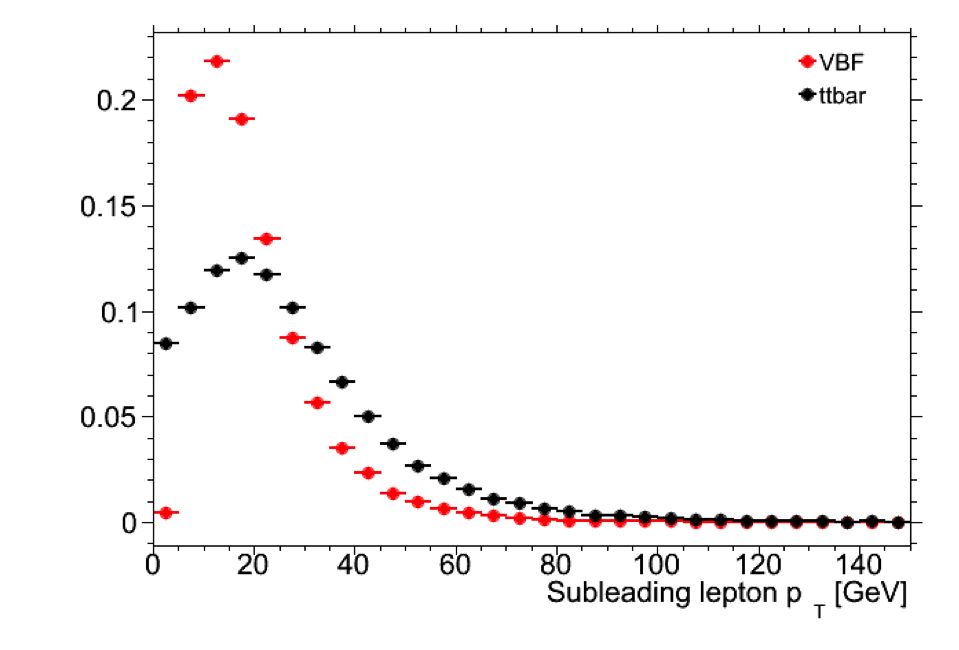
\includegraphics[width=0.6\textwidth]{figures/lepton_pt}
  \caption{A comparison of the subleading lepton $\pt$ spectrum between VBF $\HWW$ production and $t\bar{t}$ background.}
  \label{fig:leptonpt}
\end{figure}

As discussed in Chapter 2, there are multiple levels in the ATLAS trigger system, and there are different $\pT$ thresholds imposed for the leptons at each level. Additionally, some triggers have a loose selection on the isolation of the lepton (looser than that applied offline in the analysis object selection). Table~\ref{tab:single-lepton-trig} shows the $\pT$ thresholds used for single lepton triggers, while table~\ref{tab:dilepton-trig} shows the $\pT$ thresholds coming from di-lepton triggers. The single lepton trigger efficiency for muons that pass the analysis object selection is $70$\% for muons in the barrel region ($|\eta| < 1.05$) and $90$\% in the endcap region. The electron trigger efficiency increases with electron $\pT$ but the average is approximately $90$\%. These efficiencies are measured by combined performance and trigger signature groups~\cite{MuonTrigger2012,ElectronTrigger2012}.

\begin{table}[h!]
\centering
\captionsetup{justification=centering}

%\begin{tabular*}{0.480\textwidth}{p{0.075\textwidth} p{0.180\textwidth} l}
\hspace{-10pt}
\begin{tabular}{|c|c|c|}
\hline
 & Level-1 threshold & High-level threshold \\ \hline \hline
\multirow{2}{*}{Electron} & $18$ & $24i$ \\ 
 & $30$ & $60$ \\ \hline

\multirow{2}{*}{Muon} & \multirow{2}{*}{$15$} & $24i$ \\ 
& & $36$ \\ 
 \hline

\end{tabular}

\caption{
Single lepton triggers used for electrons and muons in the \HWWfull analysis. A logical ``or" of the triggers listed for each lepton type is taken. Units are in GeV, and the $i$ denotes an isolation requirement in the trigger. 
}
\label{tab:single-lepton-trig}
\end{table}

\begin{table}[h!]
\centering
\captionsetup{justification=centering}

%\begin{tabular*}{0.480\textwidth}{p{0.075\textwidth} p{0.180\textwidth} l}
\hspace{-10pt}
\begin{tabular}{|c|c|c|}
\hline
 & Level-1 threshold & High-level threshold \\ \hline \hline
$ee$ & $10$ and $10$ & $12$ and $12$ \\ \hline
$\mu\mu$ & $15$ & $18$ and $8$ \\ \hline
$e\mu$ & $10$ and $6$ & $12$ and $8$ \\ \hline
\end{tabular}

\caption{
Di-lepton triggers used for different flavor combinations in the \HWWfull analysis. The two thresholds listed refer to leading and sub-leading leptons, respectively. The di-muon trigger only requires a single lepton at level-1. 
}
\label{tab:dilepton-trig}
\end{table}

The combination of all listed triggers gives good efficiency for signal events. This efficiency is summarized in table~\ref{tab:trigeff}. The relative improvement in efficiency by adding the dilepton triggers is also shown in the same table. The largest gain comes in the $\mu\mu$ channel. Overall the trigger selection shows a good efficiency for $\HWW$ signal events.

\begin{table}[h!]
\centering
\captionsetup{justification=centering}

%\begin{tabular*}{0.480\textwidth}{p{0.075\textwidth} p{0.180\textwidth} l}
\hspace{-10pt}
\begin{tabular}{|c|c|c|}
\hline
Channel & Trigger efficiency & Gain from $2\ell$ trigger \\ \hline \hline
$ee$ & $97$\% & $9.1$\% \\ \hline
$\mu\mu$ & $89$\% & $18.5$\% \\ \hline
$e\mu$ & $95$\% & $8.3$\% \\ \hline
$\mu e$ & $81$\% & $8.2$\% \\ \hline
\end{tabular}

\caption{
Trigger efficiency for signal events and relative gain of adding a dilepton trigger on top of the single lepton trigger selection. The first lepton is the leading, while the second is the sub-leading. Efficiencies shown here are for the ggF signal in the $\Njet = 0$ category but are comparable for the VBF signal. 
}
\label{tab:trigeff}
\end{table}

\subsection{Monte Carlo samples}
\label{sec:HWWMC}

In both the gluon fusion and vector boson fusion focused analyses, modeling of signal and background processes in the signal region is an important consideration for the final interpretation of the analysis. Therefore, careful consideration must be paid to which Monte Carlo (MC) generators are used for specific processes. With the exception of the $W$+jet and multijet backgrounds, the $\mTH$ shape used as the final discriminant is taken from simulation\footnote{Many backgrounds are normalized from data, as described in section~\ref{sec:HWWbkg}.}. 

Table~\ref{tab:HWW-MC} shows the MC generators used for the signal and background processes, as well as the cross sections of each process. In order to include corrections up to next-to-leading order (NLO) in the QCD coupling constant $\alpha_{s}$, the \POWHEG~\cite{powheg1} generator is often used. In some cases, only leading order generators like \ACERMC~\cite{acermc} and \GGTOVV~\cite{gg2vv} are available for the process in question. If the process requires good modeling for very high parton multiplicities, the \SHERPA~\cite{sherpa} and \ALPGEN~\cite{alpgen} generators are used to provide merged calculations for five or fewer additional partons. These matrix element level calculations must then be additionally matched to models of the underlying event, hadronization, and parton shower. There are four generators used for this purpose: \SHERPA, \PYTHIA6~\cite{pythia6}, \PYTHIA8~\cite{pythia8}, or \HERWIG~\cite{herwig} + \JIMMY~\cite{jimmy}. The simulation additionally requires an input parton distribution function (PDF). The \CT10~\cite{ct10} PDFs are used for \SHERPA and \POWHEG simulated samples, while \CTEQ6L1~\cite{cteq} is used for \ALPGEN+\HERWIG and \ACERMC simulations. The Drell-Yan samples are reweighted to the \MRST~\cite{mrst} PDFs, as these are found to give the best agreement between data and simulation. The branching ratio for Higgs to $WW^*$ and $ZZ^*$ is computed with \PROPHECY4f~\cite{prophecy4f}, while the width of all other decays is computed with \HDECAY\cite{hdecay}. 

\begin{table}[t!]
\centering
\captionsetup{justification=centering}
\begin{tabular*}{0.75\textwidth}{
    lll p{0.25\textwidth} c
}
\dbline
\multicolumn{3}{l}{\multirow{2}{*}{Process}}
& \multicolumn{1}{l}{\multirow{2}{*}{MC generator$\nq$}}
& \multicolumn{1}{r}{$\sigma{\CDOT}\mathcal{B}$~~}
\\
&
&
&
& \multicolumn{1}{r}{(pb)~~}
\\
\sgline
\multicolumn{2}{l}{Signal }& & \\
\quad ggF    &$\HWW$                                                             && \POWHEG+\PYTHIA8      & $0.435$ \\
\quad VBF    &$\HWW$                                                             && \POWHEG+\PYTHIA8      & $0.0356$ \\
\quad $\VH$  &$\HWW$                                                             && \PYTHIA8              & $0.0253$ \\
\sgline
\multicolumn{3}{l}{$\WW$ }& & \\
\multicolumn{3}{l}{\quad $\qq{\TO}\WW$ and $qg{\TO}\WW$                          }& \POWHEG+\PYTHIA6      & $5.68$ \\ 
\multicolumn{3}{l}{\quad $gg{\TO}\WW$                                            }& \GGTOVV+\HERWIG       & $0.196$ \\
\multicolumn{3}{l}{\quad $(\qq{\TO}W){\PLUS}(\qq{\TO}W)$                         }& \PYTHIA8              & $0.480$ \\
\multicolumn{3}{l}{\quad $\qq{\TO}\WW$                                           }& \SHERPA               & $5.68$ \\
\multicolumn{3}{l}{\quad VBS $\WW{+\,}2\,\textrm{jets}$                          }& \SHERPA               & $0.0397$ \\
\sgline
\multicolumn{3}{l}{Top quarks }& & \\
\multicolumn{3}{l}{\quad $\ttbar$                                                }& \POWHEG+\PYTHIA6      & $26.6$ \\
\multicolumn{3}{l}{\quad $Wt$                                                    }& \POWHEG+\PYTHIA6      & $2.35$ \\
\multicolumn{3}{l}{\quad $tq\bar{b}$                                             }& \ACERMC+\PYTHIA6      & $28.4$ \\
\multicolumn{3}{l}{\quad $t\bar{b}$                                              }& \POWHEG+\PYTHIA6      & $1.82$ \\
\sgline
\multicolumn{3}{l}{Other dibosons ($VV$)}& & \\
\multicolumn{1}{l}{\quad $\Wg$  } &\multicolumn{2}{l}{($\pT^{\gamma}{\GT}8\GeV$) }& \ALPGEN+\HERWIG       & $369$ \\
\multicolumn{1}{l}{\quad $\Wgs$ } &\multicolumn{2}{l}{($\mll{\LE}7\GeV$)         }& \SHERPA               & $12.2$ \\ 
\multicolumn{1}{l}{\quad $\WZ$  } &\multicolumn{2}{l}{($\mll{\GT}7\GeV$)         }& \POWHEG+\PYTHIA8      & $12.7$ \\ 
%\multicolumn{2}{l}{\quad $\WZ{\PLUS}2\,\textrm{jets}$, ${\cal{O}}(\alpha_s^0)$} &($\mll{\GT}7\GeV$) & \SHERPA  & 0.013 \\
\multicolumn{3}{l}{\quad VBS $\WZ{\PLUS}2\,\textrm{jets}$                        }& \SHERPA               & $0.0126$ \\
\multicolumn{1}{l}{\quad        } & ($\mll{\GT}7\GeV$)                            &                       & \\
\multicolumn{1}{l}{\quad $\Zg$  } &\multicolumn{2}{l}{($\pT^{\gamma}{\GT}8\GeV$) }& \SHERPA               & $163$ \\
\multicolumn{1}{l}{\quad $\Zgs$ } &\multicolumn{2}{l}{(min.\ $\mll{\LE}4\GeV$)   }& \SHERPA               & $7.31$ \\
\multicolumn{1}{l}{\quad $\ZZ$  } &\multicolumn{2}{l}{($\mll{\GT}4\GeV$)         }& \POWHEG+\PYTHIA8      & $0.733$ \\
\multicolumn{3}{l}{\quad $\ZZ{\TO}\ell\ell\,\nu\nu$ ($\mll{\GT}4\GeV$)           }& \POWHEG+\PYTHIA8      & $0.504$ \\
\sgline
\multicolumn{3}{l}{Drell-Yan }& & \\
\multicolumn{1}{l}{\quad $Z$   } &\multicolumn{2}{l}{($\mll{\GT}10\GeV$)         }& \ALPGEN+\HERWIG  $\np$& $16500$ \\
\multicolumn{3}{l}{\quad VBF $Z{\PLUS}2\,\textrm{jets}$                          }& \SHERPA               & $5.36$ \\
\multicolumn{1}{l}{\quad        } & ($\mll{\GT}7\GeV$)                            &                       & \\
\dbline
\end{tabular*}
\caption{
  Monte Carlo samples used to model the signal and background processes~\cite{WW2015}. The table lists the cross section for each process, taking into account the branching ratio for the process producing two leptons. 
}
\label{tab:HWW-MC}
\end{table}


Once the basic hard scattering process is simulated, it must be passed through a detector simulation and additional pile-up events must be overlaid. The pile-up events are modeled with \PYTHIA8, and the ATLAS detector is simulated with \GEANT4~\cite{geant4}. Because of the unique phase space of the $\HWW$ analysis, events are sometimes filtered at generator level to allow for more efficient generation of relevant events. The efficiency of the trigger in MC simulation does not always match the measured efficiency in data, so trigger scale factors are applied to correct the MC efficiency to the data. The details of these corrections are given in reference~\cite{MuonTrigger2012} for muons and reference~\cite{ElectronTrigger2012} for electrons.

\section{Object selection}

In order to define the signal region, the analysis must first select the reconstructed physics objects to be considered. The details of the object reconstruction algorithms were discussed in Chapter 2, while this section gives specific selection requirements used in the $\HWW$ analysis. The first step in this process is to select a primary vertex candidates. The event's primary vertex is chosen to be the vertex with the largest sum of $\pT^2$ for its associated tracks. It is required to have at least three tracks with $\pT > 450$ \MeV. Many of the object selection cuts are then made relative to this chosen primary vertex.

\subsection{Muons}

The analysis uses combined muon candidates, where a track in the Inner Detector has been matched to a standalone track in the Muon Spectrometer. The track parameters are combined statistically in the muon reconstruction algorithm~\cite{MuonReco}. The muons are required to be within $|\eta| < 2.5$ and have a $\pT > 10 \GeV$. To reduce backgrounds coming from mis-reconstructed leptons, there are requirements on the impact parameter of the muon relative to the primary vertex. The transverse impact parameter $d_0$ is required to be small relative to its estimated uncertainty, the exact cut value being $d_0/\sigma_{d_0} < 3$. The longitudinal impact parameter $z_0$ must satisfy $\left|z_0\sin\theta\right| < 1$ mm. 

As discussed previously, the muons must also be isolated. There are two types of lepton isolations that are calculated: track-based and calorimeter-based. For muons, the track-based isolation is defined using the scalar sum  $\sum \pT$ for tracks with $\pT > 1 \GeV$ (excluding the muon track) within a cone of  $\Delta R = 0.3$ ($0.4$) around the track for muons with $\pT > 15 \GeV$ ($10 < \pT < 15 \GeV$). The final isolation requirement is made my requiring that this scalar sum be no more than a certain fraction of the muon $\pT$. This requirement varies with muon $\pT$ and the exact requirements are defined in table~\ref{tab:muonisocuts}.

The calorimeter-based muon isolation is defined using the $\sum E_{T}$ calculated from calorimeter cells with the same cone size as the track-based isolation but excluding cells within $\Delta R < 0.05$ around the muon. This isolation is also defined as a requirement on the ratio of the sum to the muon $\pT$ and varies with muon $\pT$. The requirement values as a function of $\pT$ are also given in table~\ref{tab:muonisocuts}.

The isolation requirements loosen as a function of $\pT$ to allow for larger signal acceptance. At low $\pT$, the isolation is tightened to reduce the $W$+jets background which arises from a misidentified lepton. 

\begin{table}[h!]
\centering
\captionsetup{justification=centering}

%\begin{tabular*}{0.480\textwidth}{p{0.075\textwidth} p{0.180\textwidth} l}
\hspace{-10pt}
\begin{tabular}{|c|c|c|}
\hline
$p_T$ range (GeV) & Calorimeter isolation & Track isolation\\ \hline \hline
$10-15$ & $0.06$ & $0.06$ \\ \hline
$15-20$ & $0.12$ & $0.08$ \\ \hline
$20-25$ & $0.18$ & $0.12$ \\ \hline
$> 25$ & $0.30$ & $0.12$ \\ \hline
\end{tabular}

\caption{
$\pT$ dependent isolation requirements for muons. Muons are required to have their calorimeter based or track based cone sums be less than this fraction of their $\pT$.
}
\label{tab:muonisocuts}
\end{table}

\subsection{Electrons}

Electrons are identified and reconstructed using the methods previously described in chapter 2. The electrons are required to have $|\eta| < 2.47$, and candidates in the transition region between the barrel and endcap ($1.37 < |\eta| < 1.52$) are excluded. As the muons, the electrons are required to have transverse impact parameter significance $ < 3$, while in the longitudinal direction they must have $|z_0 \sin \theta| < 0.4$ mm. Some electron requirements also vary with electron $E_{T}$, and these requirements are summarized in table~\ref{tab:elecselec}.

The isolation for electrons is defined similarly to the muons but with unique requirements on the objects included. The track-based isolation is constructed using tracks with $\pT > 400 \MeV$ with cone sizes as defined for the muons. The calorimeter-based isolation also uses the same cone size as the muon, but here the cells within a $0.125 \times 0.175$ area in $\eta \times \phi$ around the electron cluster's barycenter are excluded. The other difference with respect to muons is that the denominator of the isolation ratio is the electron $E_{T}$ rather than $\pT$. The isolation cuts very with electron $E_{T}$ and are defined in table~\ref{tab:elecselec}. The electron is also required to not be consistent with a vertex coming from a photon conversion. 


\begin{table}[h!]
\centering
\captionsetup{justification=centering}

%\begin{tabular*}{0.480\textwidth}{p{0.075\textwidth} p{0.180\textwidth} l}
\hspace{-10pt}
\begin{tabular}{|c|c|c|c|}
\hline
$p_T$ range (GeV) & Quality cut & Calorimeter isolation & Track isolation\\ \hline \hline
$10-15$ & Very tight LH & $0.20$ & $0.06$ \\ \hline
$15-20$ & Very tight LH & $0.24$ & $0.08$ \\ \hline
$20-25$ & Very tight LH & $0.28$ & $0.10$ \\ \hline
$> 25$ & Medium & $0.28$ & $0.10$ \\ \hline
\end{tabular}

\caption{
$\pT$ dependent requirements for electrons. Electrons are required to have their calorimeter based or track based cone sums be less than this fraction of their $E_{T}$.
}
\label{tab:elecselec}
\end{table}

\subsection{Jets}

Jets are clustered with the anti-$k_T$ reconstruction algorithm using a radius parameter of $R=0.4$. They are required to have a jet vertex fraction (\jvf) of at least 50\%, meaning that half of the tracks associated with the jet originated from the primary vertex. Jets with no tracks associated (i.e. those outside the acceptance of the ID) do not have this requirement applied. Jets are required to have $p_{T} > 25 \GeV$ if they are within the tracking acceptance ($|\eta| < 2.4$). Jets with $2.4 < |\eta| < 4.5$ are required to have $\pT > 30 \GeV$. This tighter requirement reduces jets from pileup in the region where \jvf\, requirements cannot be applied. The two highest $\pT$ jets in the event are referred to as the ``VBF" jets and used to compute variables used in the analysis selection. 

Identification of $b$-jets is done using the MV1 algorithm and is limited to the acceptance of the ID ($|\eta| < 2.5$)~\cite{Run1BJets}. The operating point of MV1 used is $85$\% efficient for identifying true $b$-jets. This operating point has a $10.3$\% probability of mis-tagging a light quark jet as a $b$-jet. The analysis vetoes events that contain $b$-tagged jets with $\pT > 20 \GeV$. 

\subsection{Overlap removal}

There are some cases where reconstructed objects will overlap and one will have to be chosen (for example, an electron and a jet in the calorimeter). First, the case of lepton overlap is dealt with. If an electron candidate extends into the muon spectrometer, it is removed. If a muon and electron are within $\Delta R < 0.1$ of each other, the electron is removed and the muon is kept. If two electron candidates overlap within the same radius, then the higher $E_{T}$ electron is kept. Next, the overlap between leptons and jets is considered. If an electron and jet are within $\Delta R < 0.3$ of one another, the electron is kept and the jet is removed. However, if a muon and jet overlap within $\Delta R < 0.3$, the jet is kept (as it is likely that the muon is the result of a semileptonic decay inside the jet). Once the overlap removal is complete, the final set of objects used in the analysis is defined. 

\section{Analysis selection}

This section discusses the variables used to distinguish VBF production of the Higgs in the \HWWfull final state. First, pre-selection requirements are presented. Then, the definitions of analysis variables and the cut-based signal region are shown. Finally, the BDT signal region is defined and the commonalities between the two signal regions are discussed.  


\subsection{Pre-selection}
\label{sec:vbf_presel}
Both the cut-based and BDT analyses have a common pre-selection that is applied before the signal region requirements. The requirements on leptons are common to all $\Njet$ bins. The analysis requires two oppositely charged leptons, with the leading lepton required to have $\pT > 22$ \GeV\,while the subleading lepton must have $\pT > 10$ \GeV. Next, to remove low mass $\ZDY$ events, a requirement on the dilepton mass $\mll > 10\, (12)$ \GeV\,is applied in the different (same) flavor channel. In the same flavor channels, there is an additional veto placed on the region around the Z peak, requiring that $|\mll - \mZ| > 15$ \GeV. 

There are also requirements on the amount of missing transverse momentum in the event. These are only applied in the same flavor channels, where $\ZDY$+jets production is one of the dominant backgrounds. The BDT analysis requires $\MPTj > 40 \GeV$ and $\MET > 45 \GeV$. The cut-based analysis must select more tightly on these variables to have maximal sensitivity and thus requires $\MPTj > 50 \GeV$ and $\MET > 55 \GeV$. Figure~\ref{fig:VBF_cb_met} shows the distributions of both $\MET$ and $\MPTj$ compared between data and simulation in the same flavor channels. Both variables are modeled fairly well in the bulk of the distribution, with some mis-modeling arising in the tails. Additionally, it is interesting to note that the $\ZDY\to \ell\ell$ backgrounds tends to have lower values of both variables compared to the VBF signal, as expected.

\begin{figure}[h!]
  \centering
  \captionsetup{justification=centering}
  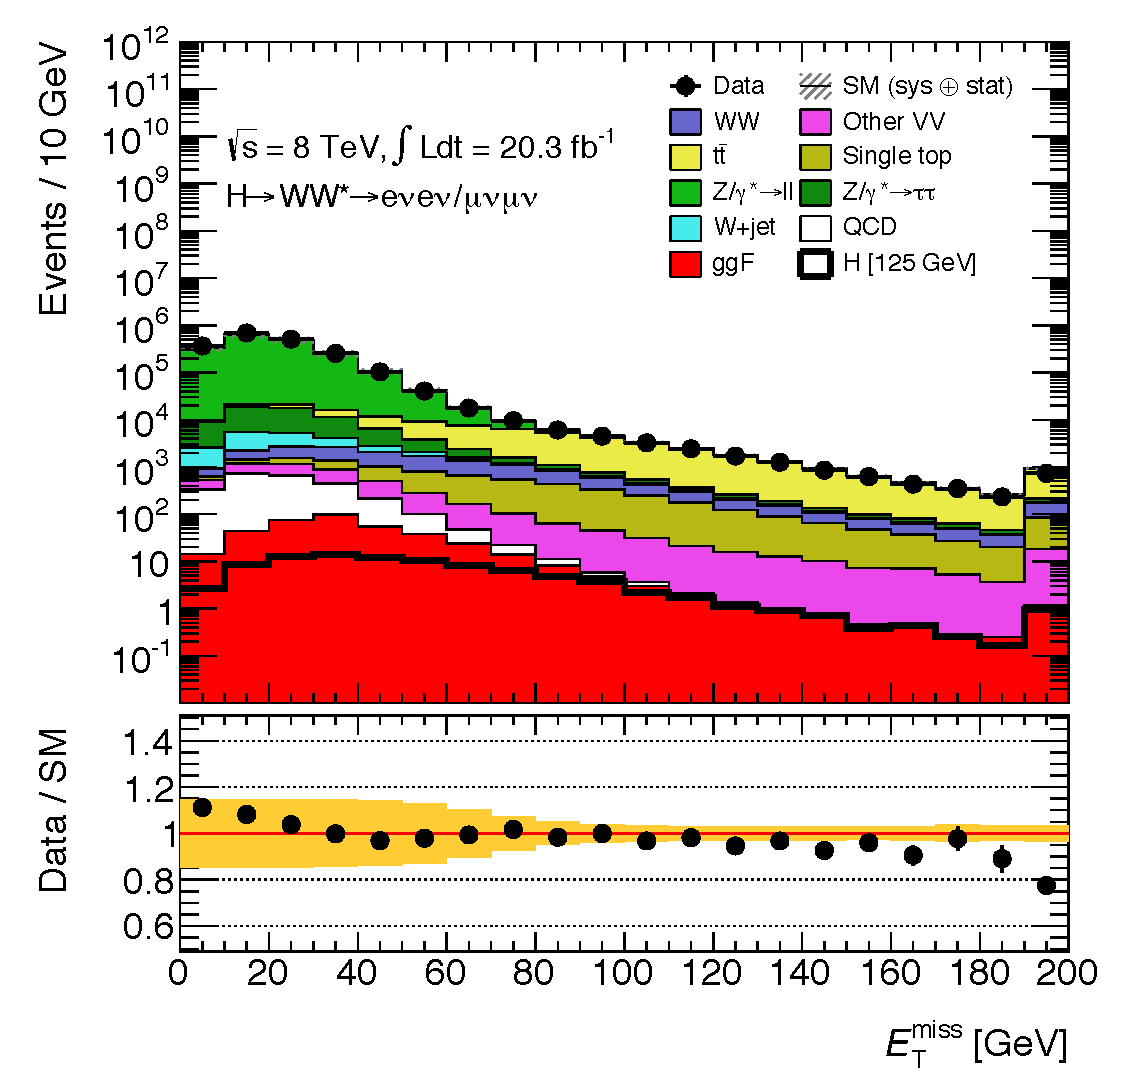
\includegraphics[width=0.49\textwidth]{figures/VBF_cb_met}
  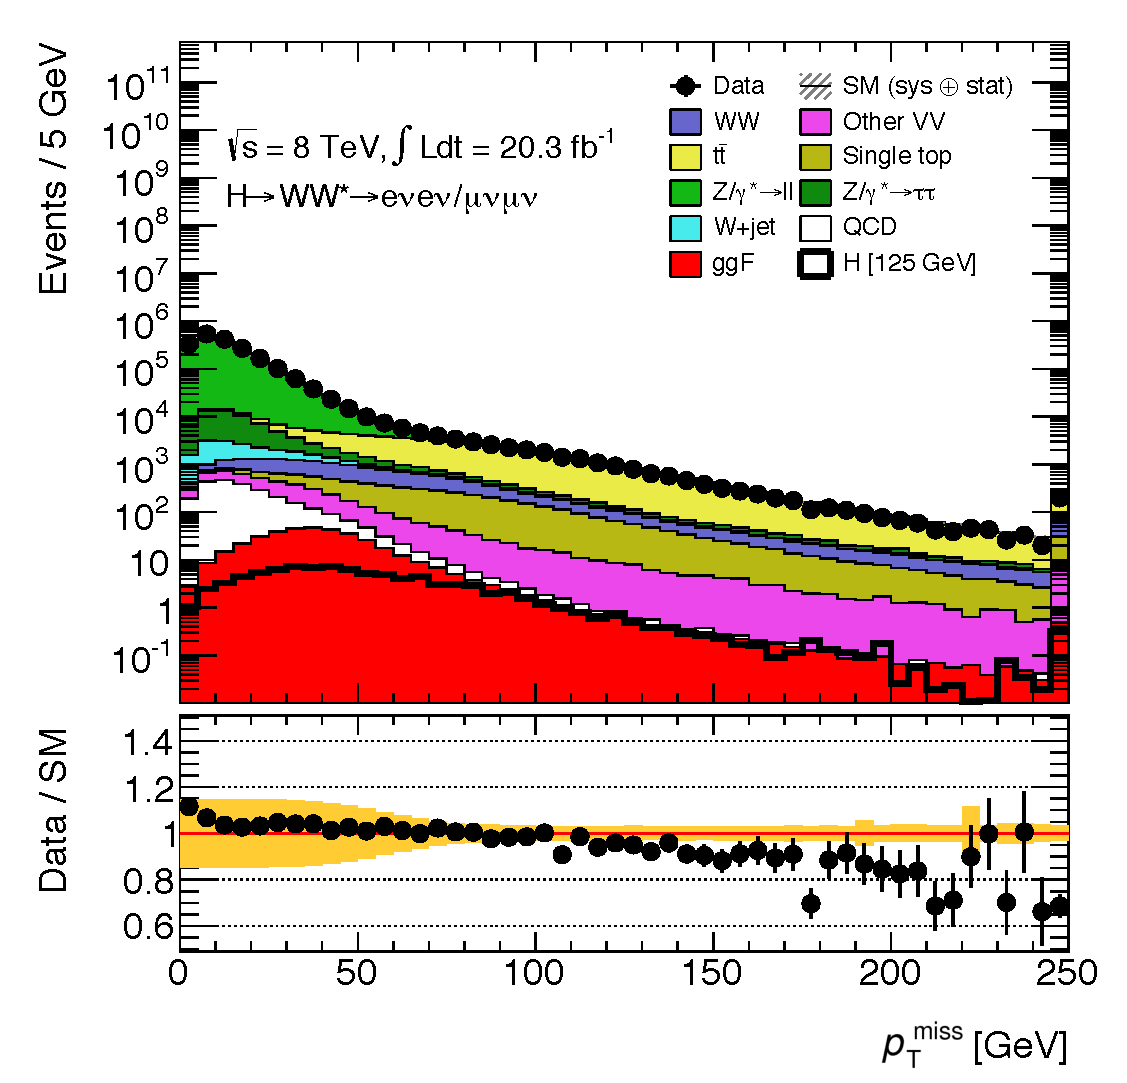
\includegraphics[width=0.49\textwidth]{figures/VBF_cb_trackmet}

  \caption{Comparisons between data and Monte Carlo simulation for the calorimeter-based $\MET$ (left) and the track-based $\MPTj$ (right) in the same flavor VBF $\HWW$ analysis channels. Both distributions are shown after the pre-selection cuts on $\mll$. The bottom panel shows the ratio between the data and the number of events expected from combining the signal and background. The hashed and orange bands include both statistical and systematic uncertainties.}
  \label{fig:VBF_cb_met}
\end{figure}

Finally, because this analysis is focused on VBF Higgs production, a requirement on the jet multiplicity is placed, with $\Njet \geq 2$. Additionally, the analysis requires that there are no jets identified as b-quarks in the event, or $\Nbjet = 0$. Figure~\ref{fig:njets} shows the jet multiplicity distributions in data and Monte Carlo simulation for both $\Njet$ and $\Nbjet$. The $\Njet$ variable is seen to be very well modeled for $\Njet \leq 7$, with some discrepancies appearing at very high jet multiplicities (where events are a small fraction of the total sample). Similarly, the $\Nbjet$ variable is modeled very well for $\Nbjet \leq 2$, with some discrepancies at higher values. 

\begin{figure}[h!]
  \centering
  \captionsetup{justification=centering}
  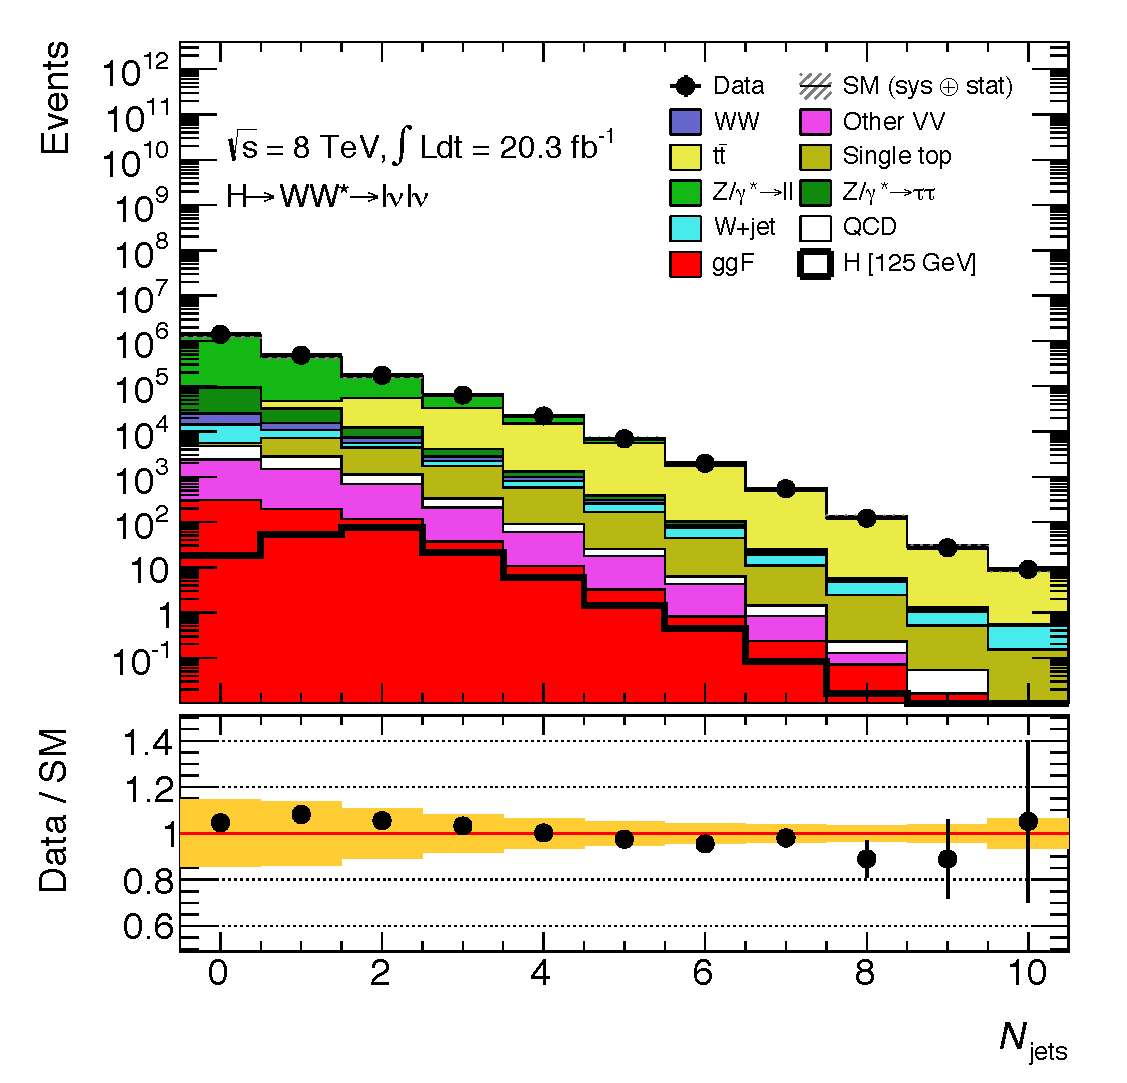
\includegraphics[width=0.49\textwidth]{figures/VBF_cb_njets}
  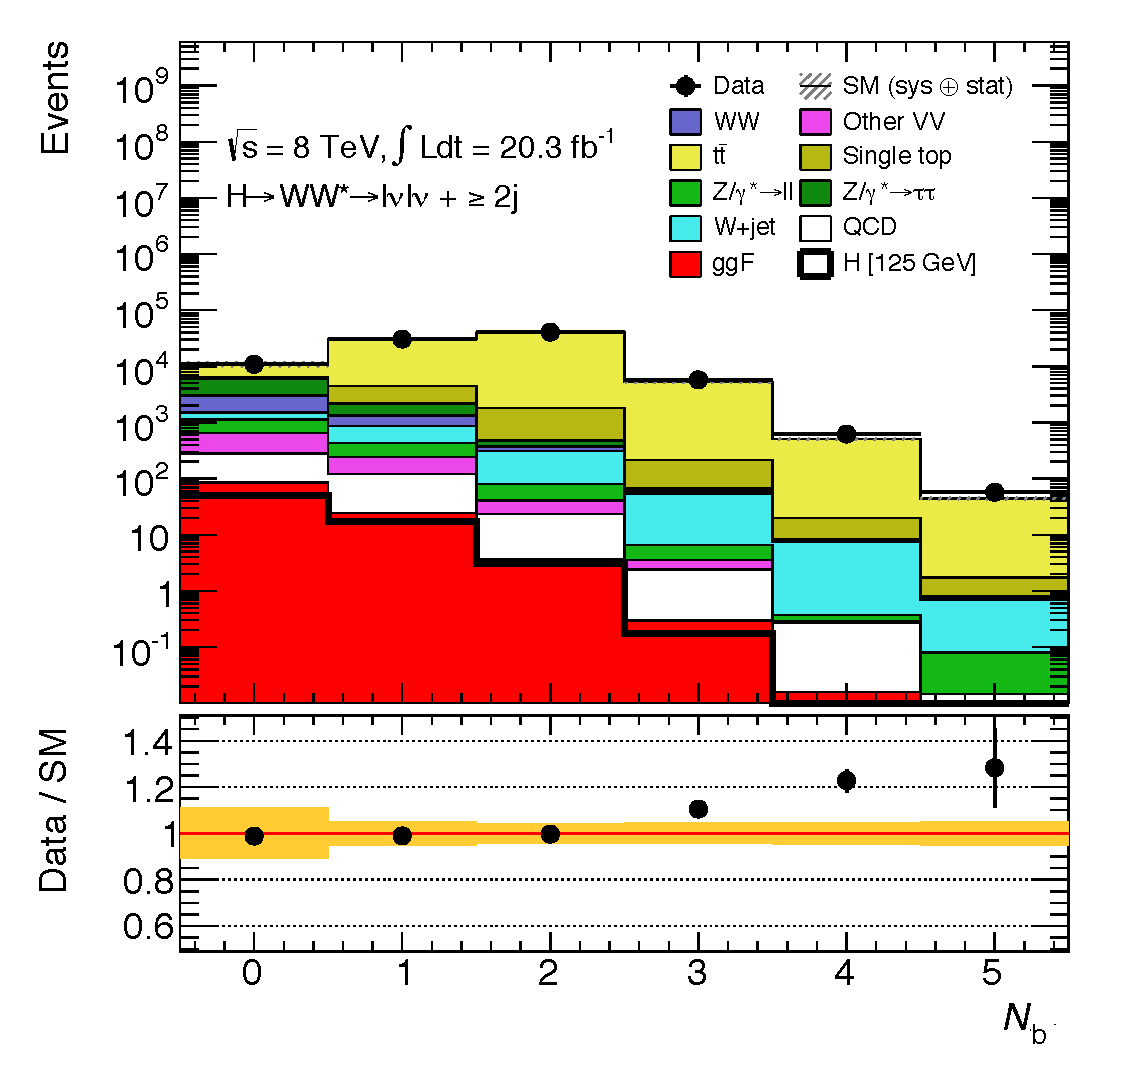
\includegraphics[width=0.49\textwidth]{figures/VBF_cb_nb}

  \caption{Comparisons between data and Monte Carlo simulation for the jet multiplicity $\Njet$ (left) and the number of $b$-tagged jets $\Nbjet$ (right) in the VBF $\HWW$ analysis. $\Njet$ is shown after the pre-selection cuts on $\mll$ and $\Nbjet$ is shown after the requirement that $\Njet \geq 2$. The bottom panel shows the ratio between the data and the number of events expected from combining the signal and background. In the $\Nbjet$ distribution, the top background is normalized using the procedures described in section~\ref{sec:topnf}. The hashed and orange bands include both statistical and systematic uncertainties.}
  \label{fig:njets}
\end{figure}

\subsection{Analysis variable definitions and cut-based selection}
\label{sec:vbf_cb_def}
The cut-based selection places sequential requirements on variables reconstructed from the VBF jets in order to increase the signal to background ratio. This section defines the variables that are used in the cut-based selection and details the requirements that are placed on these variables. 

\subsubsection{General background reduction}

Top pair production is the primary background in the $\Njet \geq 2$ bin. Even though $\Nbjet = 0$ is required, an additional variable is constructed to further suppress the top background. There is often additional QCD radiation that accompanies the $\ttbar$ system when it is produced. Therefore, a variable which tests for the presence of this additional radiation, $\pTtot$, is constructed. It is defined in equation~\ref{eqn:pttot}.
%
\begin{equation}
\vpTtot = \vpTll + \vMPTj + \sum \vpTjet
\label{eqn:pttot}
\end{equation} 
%
After pre-selection, the cut-based analysis requires the event to have $\pTtot < 15 \GeV$ to further suppress $\ttbar$ production.  

In the different flavor channels, a requirement is made to reduce the contamination from $Z\to\tau\tau$ decays. The di-$\tau$ invariant mass, $\mtt$, is constructed by assuming that the neutrinos from the $\tau$ decays were collinear with the leptons~\cite{collinear}. The analysis requires that this mass satisfy $\mtt < m_Z - 25$ \GeV so that it is not consistent with the mass of the $Z$ boson. 

\subsubsection{VBF topological cuts}
\label{sec:vbf_topocuts}

The characteristic feature of VBF production of the Higgs is the presence of two additional forward jets coming from the incoming partons which radiate the vector bosons that make the Higgs. These jets are forward because the outgoing partons still carry the longitudinal momentum of the incoming partons. Figure~\ref{fig:VBF_LeadJetEta} shows the distribution of the $\eta$ for the leading jet in a VBF event compared to a background top pair production event. As can be seen, the VBF jets tend to be more forward in $\eta$, while the $\ttbar$ jets are more central. 
%
\begin{figure}[h!]
  \vspace{20pt}
  \centering
  \hspace*{-32pt}
  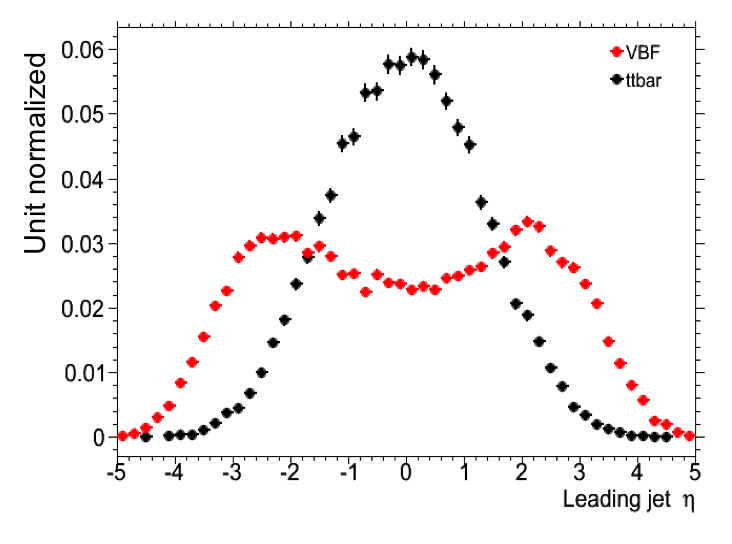
\includegraphics[width=0.6\textwidth]{figures/VBF_LeadJetEta}
  \caption{Leading jet $\eta$ in VBF $\HWW$ (red) and $\ttbar$ (black)}
  \label{fig:VBF_LeadJetEta}
\end{figure}
%
Because the cross section for VBF production is an order of magnitude smaller than gluon fusion production, these forward jets must be used in order to reduce background and achieve a good signal to background ratio. The dedicated VBF search selection requirements are constructed to maximally exploit the features of the unique VBF topology.

Requirements on the VBF jets are collectively referred to as the ``VBF topological cuts". First, a requirement on the dijet invariant mass of the VBF jets, $\mjj$, is placed, requiring $\mjj > 600 \GeV$. Next, the event is required to have a large gap in rapidity between the two VBF jets, or $\dyjj > 3.6$. Both of these are tight requirements on the presence of two forward, high $\pT$ jets moving in opposite directions in the longitudinal plane. 

Beyond requiring the presence of the two forward VBF jets, the analysis also vetoes on the presence of any additional jets that fall between the two VBF jets. This requirement is referred to as the central jet veto, or CJV. Events are vetoed if they have a third jet with $\pT > 20 \GeV$ whose rapidity is between the region defined by the two VBF jets. This requirement can be expressed in terms of a variable called the jet centrality, defined in equation~\ref{eqn:cjv}.
%
\begin{equation}
\cjv = \bigg|\, \etathirdjet - \frac{\eta_{j1} + \eta_{j2}}{2} \,\bigg|\ \Big/\ \frac{\left|\eta_{j1} - \eta_{j2}\right|}{2},
\label{eqn:cjv}
\end{equation}
%
Here, $\eta_{j1}$ and $\eta_{j2}$ are the pseudorapidities of the leading and subleading jets, respectively, while $\eta_{j3}$ is the pseudorapidity of the extra jet in the event (if one exists). Intuitively, $\cjv$ is zero when $\eta_{j3}$ is directly centered between the two jets and unity when $\eta_{j3}$ is aligned with either of the VBF jets. Thus, the CJV can be expressed as a requirement that $\cjv > 1$. 

The decay products of the Higgs tend to be central as well. Thus, the analysis also requires that both leptons in the analysis fall within the rapidity gap defined by the jets. This cut is referred to as the outside lepton veto, or OLV. Stated another way, leptons are required to have a centrality (defined analogously to that of the third jet in equation~\ref{eqn:cjv}) within the jet rapidity gap, or $\olv < 1$ for both leptons. 

\begin{figure}
  \centering
  \captionsetup{justification=centering}
  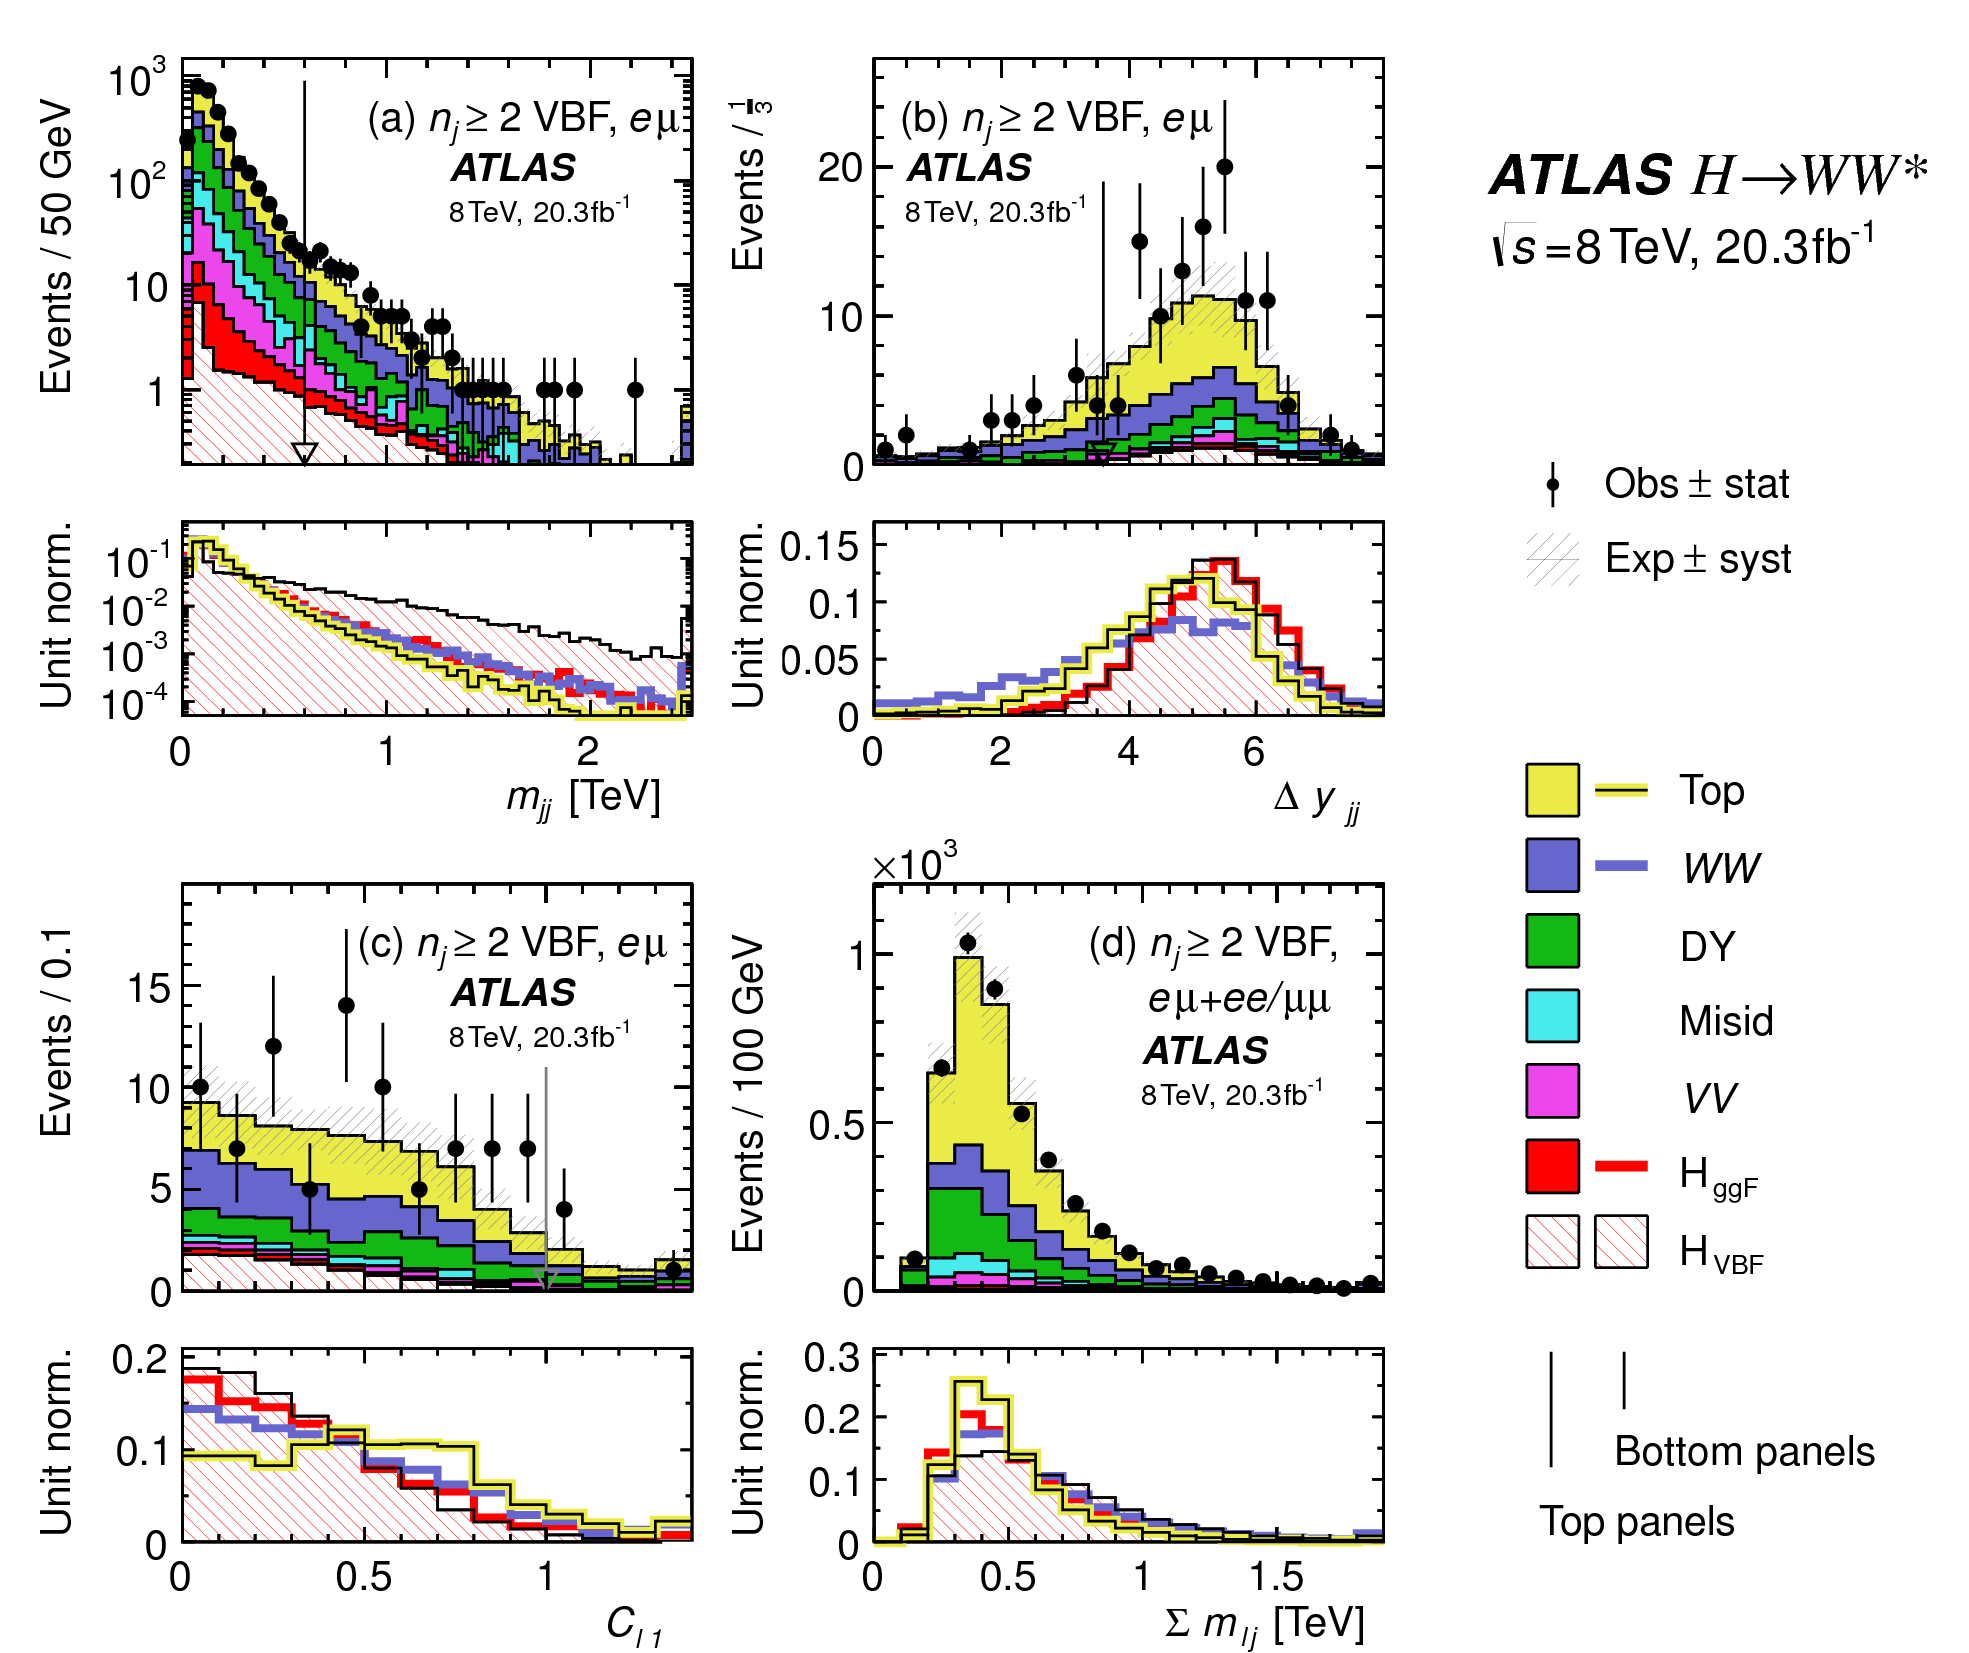
\includegraphics[width=\textwidth]{figures/VBF_vars}
  \caption{Distributions of (a) $\mjj$, (b) $\dyjj$, (c) $\olvlead$, and (d) $\mlj$, for the cut-based VBF analysis. The top panels compare simulation and data, while the bottom panels show normalized distributions for all background processes and signal for shape comparisons~\cite{WW2015}.}
  \label{fig:vbfvars}
\end{figure}

Figure~\ref{fig:vbfvars}a-c shows the $\mjj$, $\dyjj$, and $\olvlead$ variables at the stage where all previous requirements in the sequence have been made. The agreement between data and Monte Carlo is good, and the bottom panels show their power in discriminating the VBF signal from the background processes. 

The final signal region is also split into two bins of $\mjj$, with the first bin corresponding to $600 \GeV < \mjj < 1 \TeV$ and the second bin corresponding to $\mjj > 1 \TeV$. The first bin has more events but also a larger contribution from background, while the second bin has a lower expected number of events but a ~1:1 signal to background ratio. 


\subsubsection{Higgs topological cuts}

As described in section~\ref{sec:lepton_corr}, the final state leptons in \HWWfull are correlated due to the spin zero nature of the Higgs. Two requirements on dilepton kinematics are made that are common with lower multiplicity jet bins as well. The angle between leptons in the transverse plane, $\dphill$, is required to be less than $1.8$ radians. Additionally, the dilepton invariant mass, $\mll$, is required to be less than $50 \GeV$. 

\begin{figure}[h!]
  %\vspace{20pt}
  \centering
  \captionsetup{justification=centering}

   \begin{subfigure}[t]{0.5\textwidth}
        \centering
        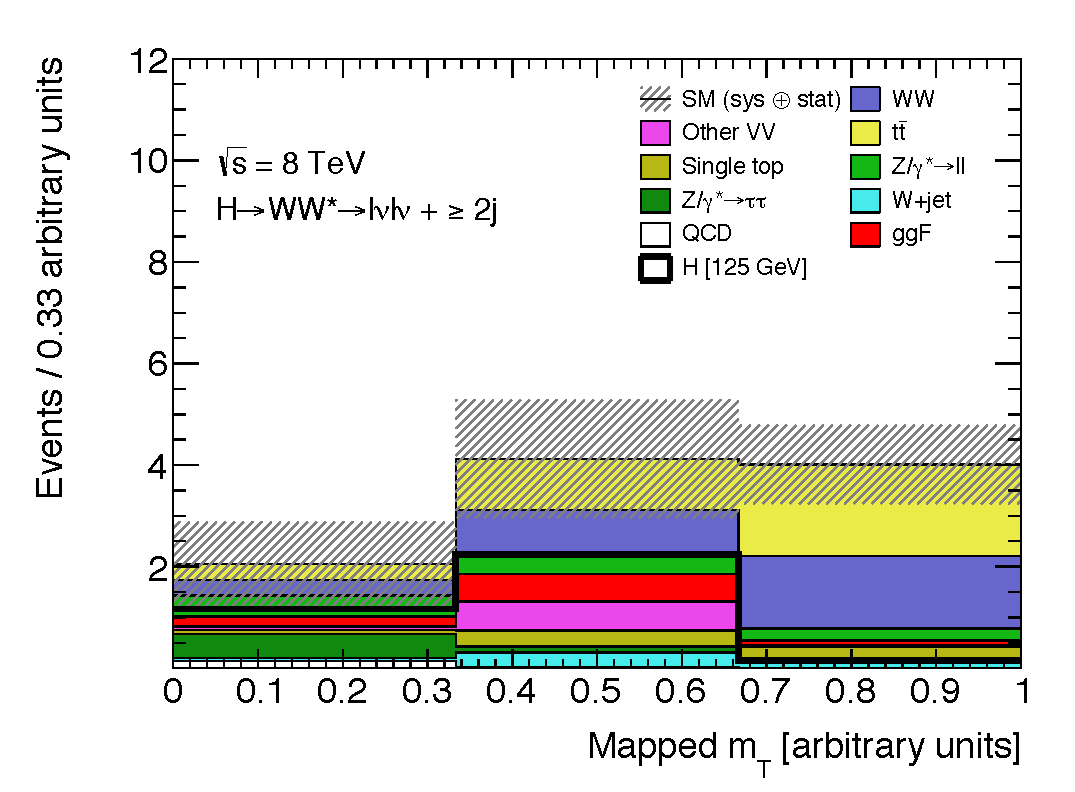
\includegraphics[width=0.95\textwidth]{figures/Mapped_MT_lowMjj}
        \caption{$600 < \mjj < 1000 \GeV$}
    \end{subfigure}%
    \begin{subfigure}[t]{0.5\textwidth}
        \centering
        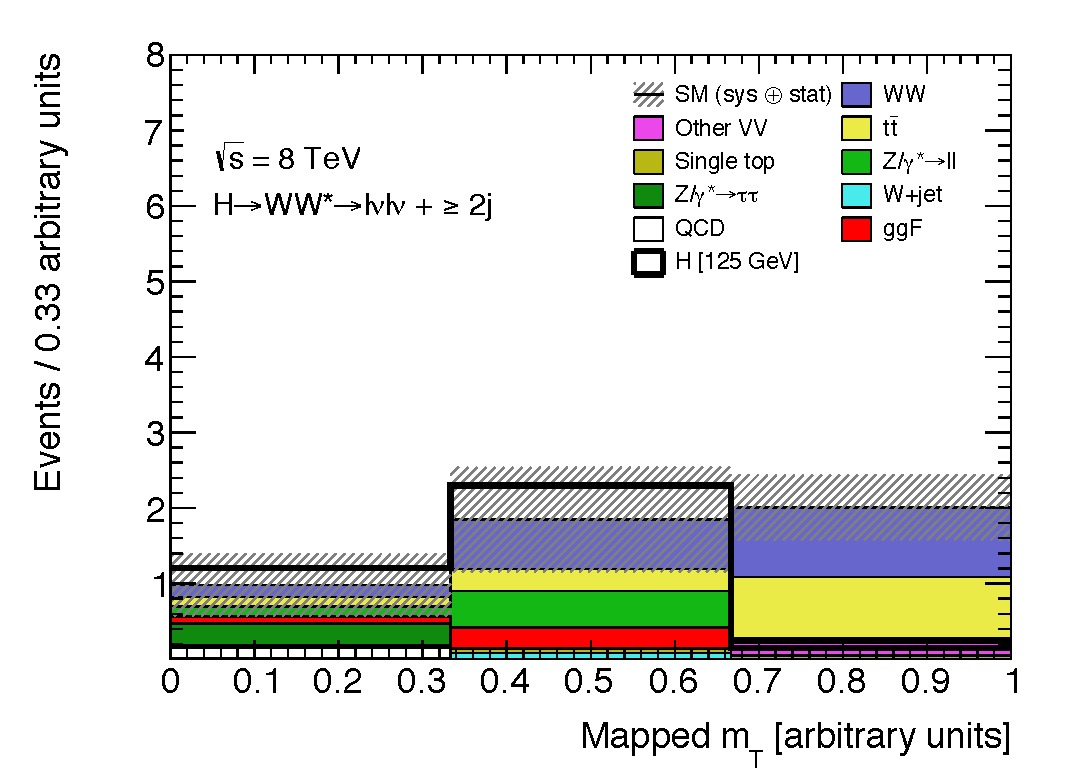
\includegraphics[width=0.95\textwidth]{figures/Mapped_MT_highMjj}
        \caption{$\mjj \geq 1000 \GeV$}
    \end{subfigure}

   \caption{$\mTH$ distribution in simulation mapped to the three bins used in the final VBF cut-based analysis fit. The bin boundaries correspond $80$ and $130 \GeV$. The solid black line corresponds to the VBF Higgs signal and is overlaid on the backgrounds to allow for shape comparison. Hashed bands include both statistical and systematic uncertainties.}
  \label{fig:VBF_mapped_mT}
\end{figure}

The cut-based analysis uses $\mTH$ as the final discriminating variable as in the ggF focused analysis. The optimal number of bins in $\mTH$ was found to be three bins, with the bin boundaries at $80$ and $130$ \GeV. Figure~\ref{fig:VBF_mapped_mT} shows the $\mTH$ distribution in the three bins used in the fit (also known as the ``mapped" $\mTH$) for both the $600 < \mjj < 1000 \GeV$ bin and the $\mjj \geq 1000 \GeV$ bin. As can be seen, both $\mjj$ bins offer discriminating power for the VBF Higgs, with the lower $\mjj$ bin providing more events and the higher $\mjj$ bin providing better signal to background ratio. 

Table~\ref{tab:vbf_cutflow_summary} shows a summary of the data and estimated signal and background yields from simulation as each requirement described above is made. The table shows how the overall signal to background ratio grows through the various selection requirements. Table~\ref{tab:vbf_cutflow_bkg} shows the background composition after each selection requirement, illustrating which backgrounds are reduced most by certain requirements. Figure~\ref{fig:eventdisplay} shows an ATLAS event display of a candidate event in the final signal region. 

\begin{table}[!htbp]
\centering%
\captionsetup{justification=centering}
%--------------------------------------------------------------------------------
%\begin{tabular*}{1\textwidth}{ l r@{$\PM$}l d{0}d{0}d{0}d{1}d{1} p{0.001\textwidth} d{0}d{0}d{0}d{0}d{0}d{0} d{1}d{1}d{0} d{2}d{1}d{1} }
\begin{tabular}{ l r@{$\PM$}l ccccc}
\dbline
&\multicolumn{7}{c}{Summary}
\\
\clineskip\cline{2-8}
\multicolumn{1}{p{0.165\textwidth}}{Selection}
& \multicolumn{2}{p{0.050\textwidth}}{$\Nobs/\Nbkg\nq$}
& \multicolumn{1}{p{0.040\textwidth}}{$\Nobs\nq\no$}
& \multicolumn{1}{p{0.040\textwidth}}{$\Nbkg\np$}
& \multicolumn{3}{p{0.125\textwidth}}{~~~~~~~~$N_{\rm signal}$}
\\
\multicolumn{2}{l}{}
& 
& 
& 
& \multicolumn{1}{l}{$\NggF\no$}
& \multicolumn{1}{l}{$\NVBF\no$}
& \multicolumn{1}{l}{$\NVH\no$}
\\
\sgline
$\DFchan$ sample                           &$1.00 $& $0.00 $&$61434$ &$61180  $& $85   $&$32   $&$26  $    \\
$\quad\Nbjet{\EQ}0$                        &$1.02 $& $0.01 $&$ 7818$ &$ 7700  $& $63   $&$26   $&$16  $  \\
$\quad\pTtot{\LT}15$                       &$1.03 $& $0.01 $&$ 5787$ &$ 5630  $& $46   $&$23   $&$13  $  \\
$\quad\mtt{\LT}\mZ{\MINUS}25\nq$           &$1.05 $& $0.02 $&$ 3129$ &$ 2970  $& $40   $&$20   $&$ 9.9$ \\
$\quad\mjj{\GT}600$                        &$1.31 $& $0.12 $&$  131$ &$  100  $& $ 2.3 $&$ 8.2 $& $-$ \\
$\quad\dyjj{\GT}3.6$                       &$1.33 $& $0.13 $&$  107$ &$   80  $& $ 2.1 $&$ 7.9 $& $-$ \\
$\quad\cjv{\GT}1$                          &$1.36 $& $0.18 $&$   58$ &$   43  $& $ 1.3 $&$ 6.6 $& $-$ \\
$\quad\olvlead{\LT}1$, $\olvsublead{\LT}1$ &$1.42 $& $0.20 $&$   51$ &$   36  $& $ 1.2 $&$ 6.4 $& $-$ \\
$\quad{\mll, \dphill, \mTH}$               &$2.53 $& $0.71 $&$   14$ &$    5.5$& $ 0.8 $&$ 4.7 $& $-$  \\
\sgline                                     $     $  $     $ $     $  $       $  $     $ $     $                     
$\SFchan$ sample                           &$0.99 $& $0.01 $&$26949$ &$27190  $& $31   $&$14   $&$10.1$  \\
$\quad\Nbjet, \pTtot, \mtt\nq$             &$1.03 $& $0.03 $&$ 1344$ &$ 1310  $& $13   $&$ 8.0 $&$ 4.0$ \\
$\quad\mjj, \dyjj, \cjv, \olv$             &$1.39 $& $0.28 $&$   26$ &$   19  $& $ 0.4 $&$ 2.9 $&$ 0.0$ \\
$\quad{\mll, \dphill, \mTH}$               &$1.63 $& $0.69 $&$    6$ &$    3.7$& $ 0.3 $&$ 2.2 $&$ 0.0$ \\
\dbline                                                                                                 
\end{tabular}%                                                                                    
%--------------------------------------------------------------------------                        
         
\caption{
  Summary of event selection for the $\NjetGEtwo$ VBF analysis in
  the $8\TeV$ cut-based analysis~\cite{WW2015}.
}
\label{tab:vbf_cutflow_summary}                                                                                     
\end{table}  

\begin{table}[!htbp]

\centering%
\captionsetup{justification=centering}
%--------------------------------------------------------------------------------
%\begin{tabular*}{1\textwidth}{ l r@{$\PM$}l d{0}d{0}d{0}d{1}d{1} p{0.001\textwidth} d{0}d{0}d{0}d{0}d{0}d{0} d{1}d{1}d{0} d{2}d{1}d{1} }
\scalebox{0.85}
{
\begin{tabular}{cccccc ccc ccc }
\dbline
&\multicolumn{10}{c}{Composition of $\Nbkg$}
\\
\clineskip\cline{2-11}\clineskip
& \multicolumn{2}{c}{$\NWW$}
& \multicolumn{2}{c}{$\Ntop$}
& \multicolumn{2}{c}{$\Nfakes$}
& \multicolumn{1}{c}{$\NVV$}
& \multicolumn{3}{c}{$\Ndrellyan$}
\\
& $\NWWqcd$ 
& $\NWWew$ 
& $\Nttbar$
& $\Nt$
& $\NWj$
& $\Njj$
& $\NVV$
& $\Nll$
& $\Ntautauqcd$
& $\Ntautauew$
\\
\sgline
$\DFchan$ sample                           &$1350   $& $68   $&$51810   $&$2970   $&$847   $&$308   $&$380       $&$ 51   $&$3260   $&$46   $\\
$\quad\Nbjet{\EQ}0$                        &$ 993   $& $43   $&$ 3000   $&$ 367   $&$313   $&$193   $&$273       $&$ 35   $&$2400   $&$29   $\\
$\quad\pTtot{\LT}15$                       &$ 781   $& $38   $&$ 1910   $&$ 270   $&$216   $&$107   $&$201       $&$ 27   $&$2010   $&$23   $\\
$\quad\mtt{\LT}\mZ{\MINUS}25\nq$           &$ 484   $& $22   $&$ 1270   $&$ 177   $&$141   $&$ 66   $&$132       $&$  7.6 $&$ 627   $&$ 5.8 $\\
$\quad\mjj{\GT}600$                        &$  18   $& $ 8.9 $&$   40   $&$   5.3 $&$  1.8 $&$  2.4 $&$  5.1     $&$  0.1 $&$  15   $&$ 1.0 $\\
$\quad\dyjj{\GT}3.6$                       &$  11.7 $& $ 6.9 $&$   35   $&$   5.0 $&$  1.6 $&$  2.3 $&$  3.3     $&  $-$ &$  11.6 $& $0.8 $\\
$\quad\cjv{\GT}1$                          &$   6.9 $& $ 5.6 $&$   14   $&$   3.0 $&$  1.3 $&$  1.3 $&$  2.0     $&  $-$ &$   6.8 $& $0.6 $\\
$\quad\olvlead{\LT}1$, $\olvsublead{\LT}1$ &$   5.9 $& $ 5.2 $&$   10.8 $&$   2.5 $&$  1.3 $&$  1.3 $&$  1.6     $&  $-$ &$   5.7 $& $0.6 $\\
$\quad{\mll, \dphill, \mTH}$               &$   1.0 $& $ 0.5 $&$    1.1 $&$   0.3 $&$  0.3 $&$  0.3 $&$  0.6     $&  $-$ &$   0.5 $& $0.2 $\\
\sgline                               
$\SFchan$ sample                           &$ 594   $& $37   $&$23440   $&$1320   $&$230   $& $ 8.6 $&$137       $&$690   $&$ 679   $&$16   $\\
$\quad\Nbjet, \pTtot, \mtt\nq$             &$ 229   $& $12.0 $&$  633   $&$  86   $&$ 26   $& $ 0.9 $&$ 45       $&$187   $&$  76   $&$ 1.5 $\\
$\quad\mjj, \dyjj, \cjv, \olv$             &$   3.1 $& $ 3.1 $&$    5.5 $&$   1.0 $&$  0.2 $& $ 0.0 $&$  0.7     $&$  3.8 $&$   0.7 $&$ 0.1 $\\
$\quad{\mll, \dphill, \mTH}$               &$   0.4 $& $ 0.2 $&$    0.6 $&$   0.2 $&$  0.2 $& $ 0.0 $&$  0.1     $&$  1.5 $&$   0.3 $&$ 0.1 $\\
\dbline                                                                                                 
\end{tabular}%                                                                                    
%--------------------------------------------------------------------------                        
}
\caption{
  Background composition after each requirement in the $\NjetGEtwo$ VBF analysis in
  the $8\TeV$ cut-based analysis~\cite{WW2015}.
}
\label{tab:vbf_cutflow_bkg}                                                                                     
\end{table}  

\begin{comment}
\begin{sidewaystable}[!htbp]
\scalebox{0.9}
{\small
  \centering%
%--------------------------------------------------------------------------------
%\begin{tabular*}{1\textwidth}{ l r@{$\PM$}l d{0}d{0}d{0}d{1}d{1} p{0.001\textwidth} d{0}d{0}d{0}d{0}d{0}d{0} d{1}d{1}d{0} d{2}d{1}d{1} }
\begin{tabular*}{1\textwidth}{ l r@{$\PM$}l ccccc p{0.001\textwidth} cccccc ccc ccc }
\dbline
&\multicolumn{7}{c}{Summary}
&&\multicolumn{10}{c}{Composition of $\Nbkg$}
\\
\clineskip\cline{2-8}\cline{10-19}\clineskip
\multicolumn{1}{p{0.165\textwidth}}{Selection}
& \multicolumn{2}{p{0.050\textwidth}}{$\Nobs/\Nbkg\nq$}
& \multicolumn{1}{p{0.040\textwidth}}{$\Nobs\nq\no$}
& \multicolumn{1}{p{0.040\textwidth}}{$\Nbkg\np$}
& \multicolumn{3}{p{0.125\textwidth}}{~~~~~~$N_{\rm signal}$}
&
& \multicolumn{2}{l}{~~~~~$\NWW$}
& \multicolumn{2}{l}{~~~~~$\Ntop$}
& \multicolumn{2}{l}{~\,$\Nfakes$}
& \multicolumn{1}{l}{$\NVV$}
& \multicolumn{3}{l}{~~~~~~~$\Ndrellyan$}
\\
\multicolumn{2}{l}{}
& 
& 
& 
& \multicolumn{1}{l}{$\NggF\no$}
& \multicolumn{1}{l}{$\NVBF\no$}
& \multicolumn{1}{l}{$\NVH\no$}
&
& \multicolumn{1}{p{0.020\textwidth}}{$\NWWqcd\np$}
& \multicolumn{1}{p{0.030\textwidth}}{$\NWWew$}
& \multicolumn{1}{p{0.020\textwidth}}{~~$\Nttbar\nq$}
& \multicolumn{1}{p{0.015\textwidth}}{$\Nt\nq$}
& \multicolumn{1}{p{0.020\textwidth}}{$\NWj\nq$}
& \multicolumn{1}{p{0.020\textwidth}}{$\Njj\np$}
& %\multicolumn{1}{p{0.020\textwidth}}{$~\,\NVV\nq$}
& \multicolumn{1}{p{0.020\textwidth}}{$\!\Nll\nq$}
& \multicolumn{1}{p{0.020\textwidth}}{$~\,\Ntautauqcd\nq$}
& \multicolumn{1}{p{0.020\textwidth}}{$~\,\Ntautauew\nq$}
\\
\sgline
$\DFchan$ sample                           &1.00 &0.00 &61434 &61180   &85   &32   &26   &&1350   &68   &51810   &2970   &847   &308   &380       & 51   &3260   &46   \\
$\quad\Nbjet{\EQ}0$                        &1.02 &0.01 & 7818 & 7700   &63   &26   &16   && 993   &43   & 3000   & 367   &313   &193   &273       & 35   &2400   &29   \\
$\quad\pTtot{\LT}15$                       &1.03 &0.01 & 5787 & 5630   &46   &23   &13   && 781   &38   & 1910   & 270   &216   &107   &201       & 27   &2010   &23   \\
$\quad\mtt{\LT}\mZ{\MINUS}25\nq$           &1.05 &0.02 & 3129 & 2970   &40   &20   & 9.9 && 484   &22   & 1270   & 177   &141   & 66   &132       &  7.6 & 627   & 5.8 \\
$\quad\mjj{\GT}600$                        &1.31 &0.12 &  131 &  100   & 2.3 & 8.2 & $-$ &&  18   & 8.9 &   40   &   5.3 &  1.8 &  2.4 &  5.1     &  0.1 &  15   & 1.0 \\
$\quad\dyjj{\GT}3.6$                       &1.33 &0.13 &  107 &   80   & 2.1 & 7.9 & $-$ &&  11.7 & 6.9 &   35   &   5.0 &  1.6 &  2.3 &  3.3     &  $-$ &  11.6 & 0.8 \\
$\quad\cjv{\GT}1$                          &1.36 &0.18 &   58 &   43   & 1.3 & 6.6 & $-$ &&   6.9 & 5.6 &   14   &   3.0 &  1.3 &  1.3 &  2.0     &  $-$ &   6.8 & 0.6 \\
$\quad\olvlead{\LT}1$, $\olvsublead{\LT}1$ &1.42 &0.20 &   51 &   36   & 1.2 & 6.4 & $-$ &&   5.9 & 5.2 &   10.8 &   2.5 &  1.3 &  1.3 &  1.6     &  $-$ &   5.7 & 0.6 \\
$\quad{\mll, \dphill, \mTH}$               &2.53 &0.71 &   14 &    5.5 & 0.8 & 4.7 & $-$ &&   1.0 & 0.5 &    1.1 &   0.3 &  0.3 &  0.3 &  0.6     &  $-$ &   0.5 & 0.2 \\
\sgline                                                                                                 
$\SFchan$ sample                           &0.99 &0.01 &26949 &27190   &31   &14   &10.1 && 594   &37   &23440   &1320   &230   &  8.6 &{\rm~137} &690   & 679   &16   \\
$\quad\Nbjet, \pTtot, \mtt\nq$             &1.03 &0.03 & 1344 & 1310   &13   & 8.0 & 4.0 && 229   &12.0 &  633   &  86   & 26   &  0.9 & 45       &187   &  76   & 1.5 \\
$\quad\mjj, \dyjj, \cjv, \olv$             &1.39 &0.28 &   26 &   19   & 0.4 & 2.9 & 0.0 &&   3.1 & 3.1 &    5.5 &   1.0 &  0.2 &  0.0 &  0.7     &  3.8 &   0.7 & 0.1 \\
$\quad{\mll, \dphill, \mTH}$               &1.63 &0.69 &    6 &    3.7 & 0.3 & 2.2 & 0.0 &&   0.4 & 0.2 &    0.6 &   0.2 &  0.2 &  0.0 &  0.1     &  1.5 &   0.3 & 0.1 \\
\dbline                                                                                                 
\end{tabular*}%                                                                                    
%--------------------------------------------------------------------------                        
}             
\caption{
  Event selection for the $\NjetGEtwo$ VBF analysis in
  the $8\TeV$ cut-based analysis~\cite{WW2015}.
}
\label{tab:vbf_cutflow}                                                                                     
\end{sidewaystable}  
\end{comment}

\begin{figure}[h!]
  \centering
  \captionsetup{justification=centering}
  \includegraphics[width=\textwidth]{figures/eventdisplay}

  \caption{Event display of a VBF candidate event~\cite{WW2015}.}
  \label{fig:eventdisplay}
\end{figure}                                                                                     


\subsection{BDT-based selection}
\label{sec:vbf_bdt_def}
The boosted decision tree based analysis uses many of the variables defined in the cut-based selection as inputs to the BDT. The output BDT score ($\bdt$) is used as the final discriminant rather than $\mTH$\footnote{For the final discriminant analysis, the $\bdt$ distribution is divided into four bins, with boundaries at $[-1, -0.48, -0.3, 0.78, 1]$.}. The BDT is trained with the VBF $\HWW$ simulation as the signal samples and all other processes as background, including ggF $\HWW$ production. While the BDT based analysis is ultimately treated as a separate result, it has significant overlap with the cut-based selection. 

\subsubsection{Pre-training selection and BDT inputs}
Before training, the common pre-selection cuts described in section~\ref{sec:vbf_presel} are applied. Additionally, the central jet veto and outside lepton veto described in section~\ref{sec:vbf_topocuts} are applied. The BDT has eight input variables, six of which are also variables that are used in the cut-based analysis. The six shared variables are $\pTtot$, $\mjj$, $\dyjj$, $\mll$, $\dphill$, and $\mTH$. The seventh variable input in the BDT is a combination of the variables used to define the OLV in the cut-based analysis. The BDT uses as input the sum of lepton centralities, or $\sum\olv = \olvlead + \olvsublead$. The final BDT input variable, $\mlj$, is constructed to account for the correlations between the jets and leptons in the event. It is the sum of the invariant masses of all four possible lepton-jet combinations. Table~\ref{tab:vbfcuts} summarizes the cuts applied for the cut-based and analyses, as well as which variables are used as input to the BDT.

\begin{table}[h!]
\centering
\captionsetup{justification=centering}
\begin{tabular}{|c|c|c|c|}
\hline
Category & Selection & Cut-based value & BDT-based value \\ \hline
\multirow{10}{*}{Pre-selection} & Leptons & \multicolumn{2}{c|}{$2$ oppositely charged} \\ \cline{2-4}
& Leading lepton $\pT$ & \multicolumn{2}{c|}{ $> 22 \GeV$} \\ \cline{2-4}
& Subleading lepton $\pT$ & \multicolumn{2}{c|}{ $> 10 \GeV$} \\ \cline{2-4}
& $\mll$ & \multicolumn{2}{c|}{ \specialcell{$>10\,(12) \GeV$ for $e\mu/\mu e$ ($ee/\mu\mu$) \\ $|\mll - m_{Z}| > 15 \GeV$ for $ee/\mu\mu$}} \\ \cline{2-4}
& \specialcell{$\MET$  \\($ee/\mu\mu$ only)} & $> 55 \GeV$ & $> 45 \GeV$  \\ \cline{2-4}
& \specialcell{$\MPTj$  \\($ee/\mu\mu$ only)} & $> 50 \GeV$ & $> 40 \GeV$ \\ \cline{2-4}
& $b$-veto & \multicolumn{2}{c|}{$\Nbjet = 0$} \\ \hline
Bkg. rejection & $\pTtot$ & $< 15 \GeV$ & Input \\ \hline
\multirow{5}{*}{VBF topology} & $\mjj$ & $> 600 \GeV$ & Input \\ \cline{2-4}
& $\dyjj$ & $> 3.6$ & Input \\ \cline{2-4}
& CJV and OLV & \multicolumn{2}{c|}{applied} \\ \cline{2-4}
& $\sum \olv$ & - & Input \\ \cline{2-4}
& $\mlj$ & - & Input \\ \hline
\multirow{5}{*}{Higgs topology} & $\mll$ & $ < 50 \GeV$ & Input \\ \cline{2-4}
& $\dphill$ & $< 1.8$ & Input \\ \cline{2-4}
& $\mTH$ & \specialcell{Three bins with boundaries\\ at $80$ and $130 \GeV$} & Input \\ \hline
\end{tabular}
\caption{Summary of selections for the cut-based and BDT signal regions. ``Input" denotes variables used as input to the BDT algorithm. Definitions and explanations of the variables can be found in sections~\ref{sec:vbf_cb_def} and~\ref{sec:vbf_bdt_def}.}
\label{tab:vbfcuts}
\end{table}

Figure~\ref{fig:vbfvars}d shows the agreement between data and simulation for the $\mlj$ variable, as well as showing its discriminating power. Figure~\ref{fig:vbf_bdt_htopo} shows the distributions of the Higgs topological variables that are shared between the cut-based and BDT analyses. Figure~\ref{fig:vbf_bdt_vbftopo} shows the distributions of the VBF topological variables shared between the cut-based and BDT analyses. In both cases, the VBF yield has been scaled by a factor of 50 to better show the shape difference compared to the backgrounds. 

 

\begin{figure}[h!]
  \centering
  \captionsetup{justification=centering}
  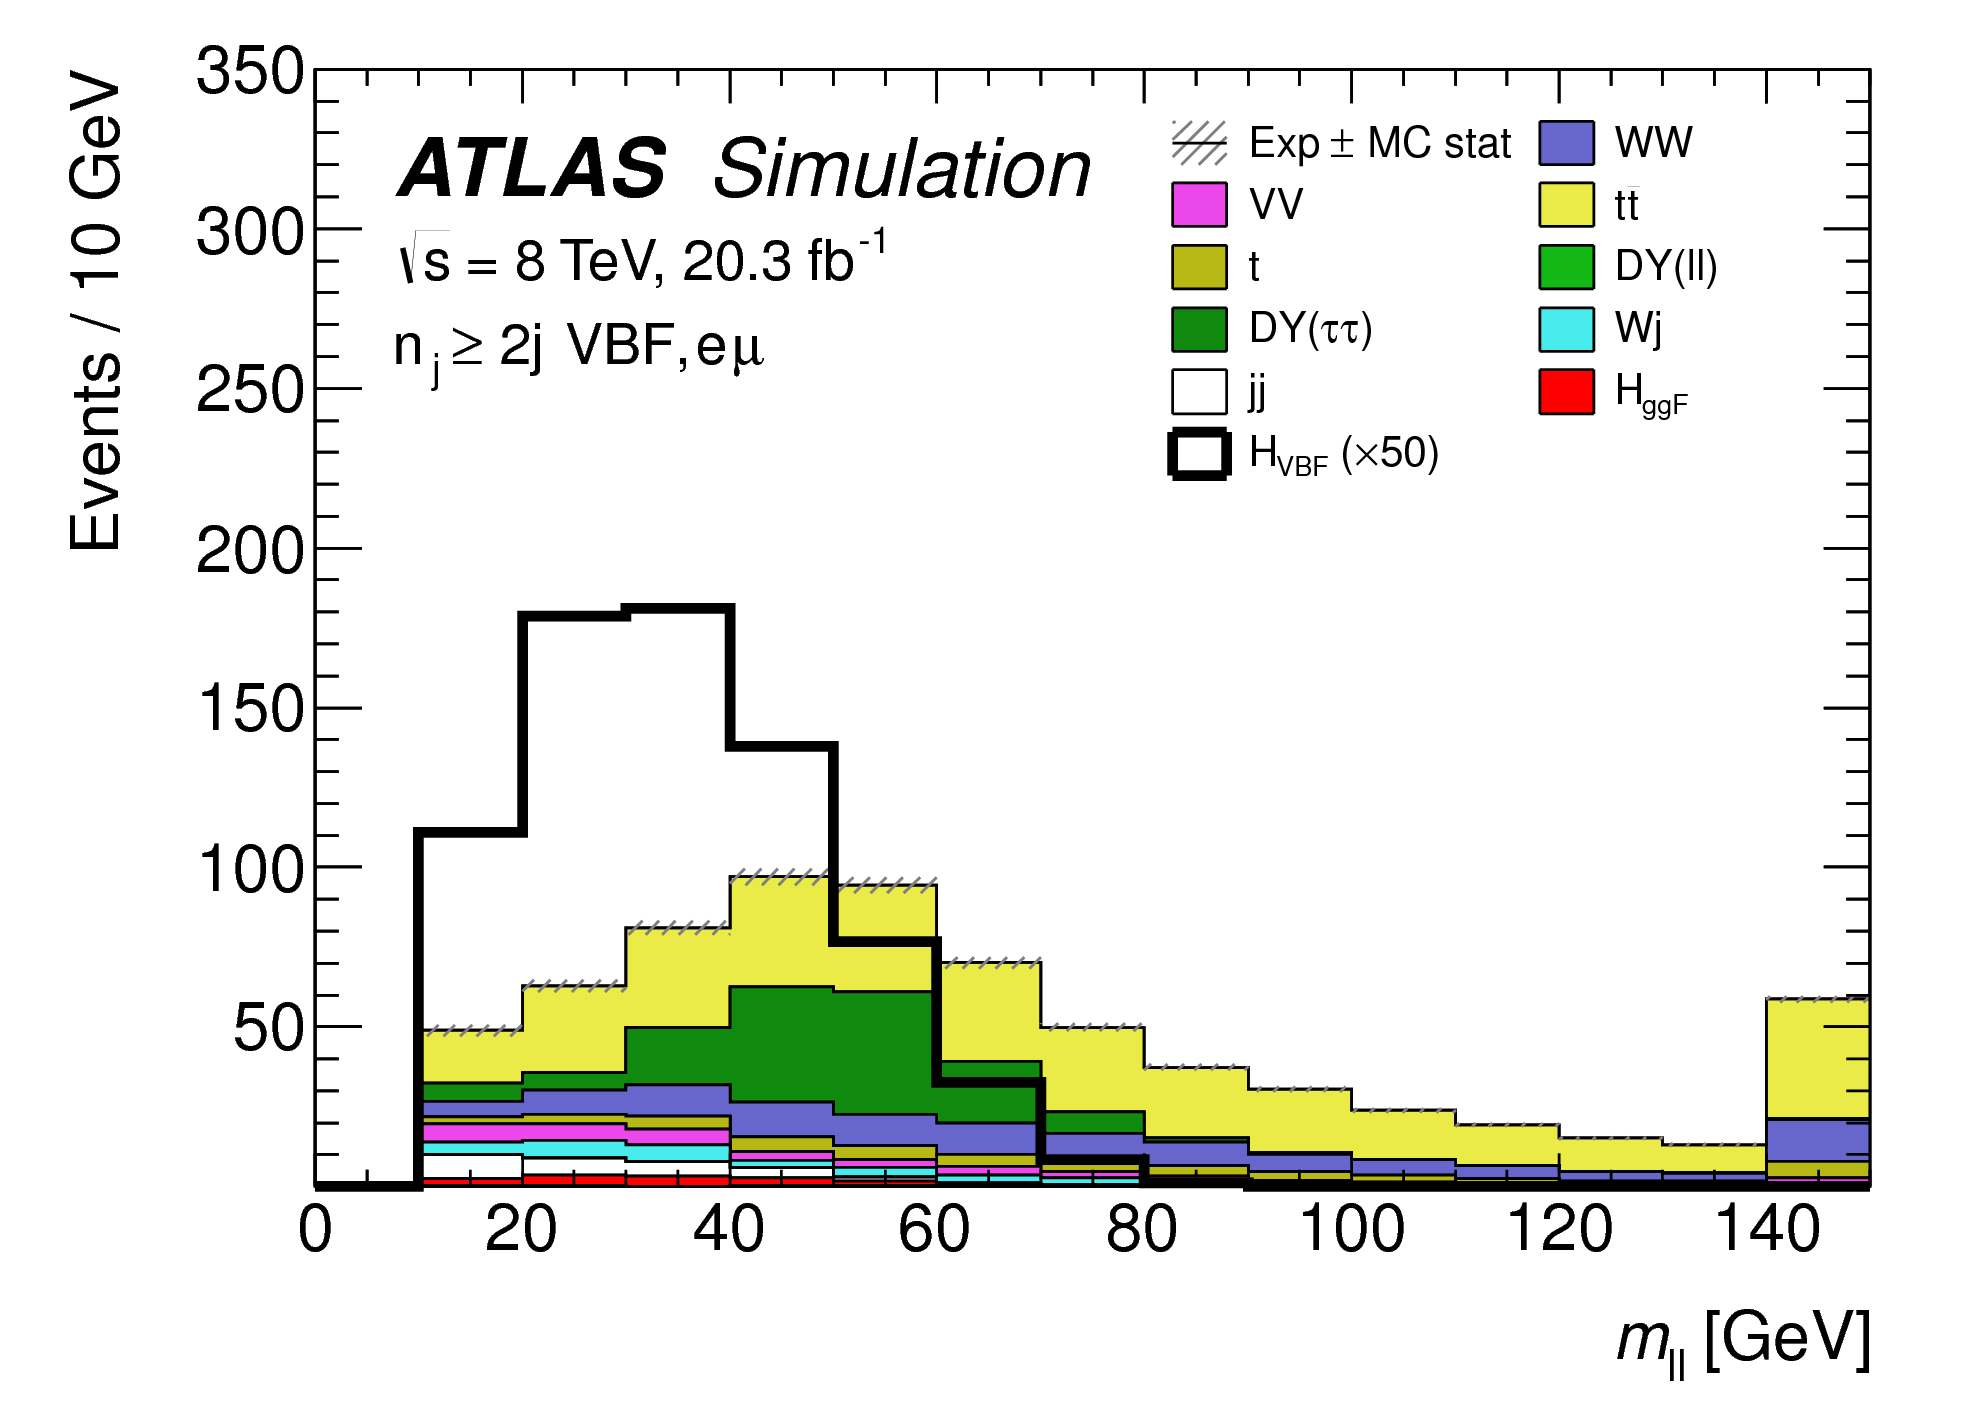
\includegraphics[width=0.45\textwidth]{figures/BDT_mll}
  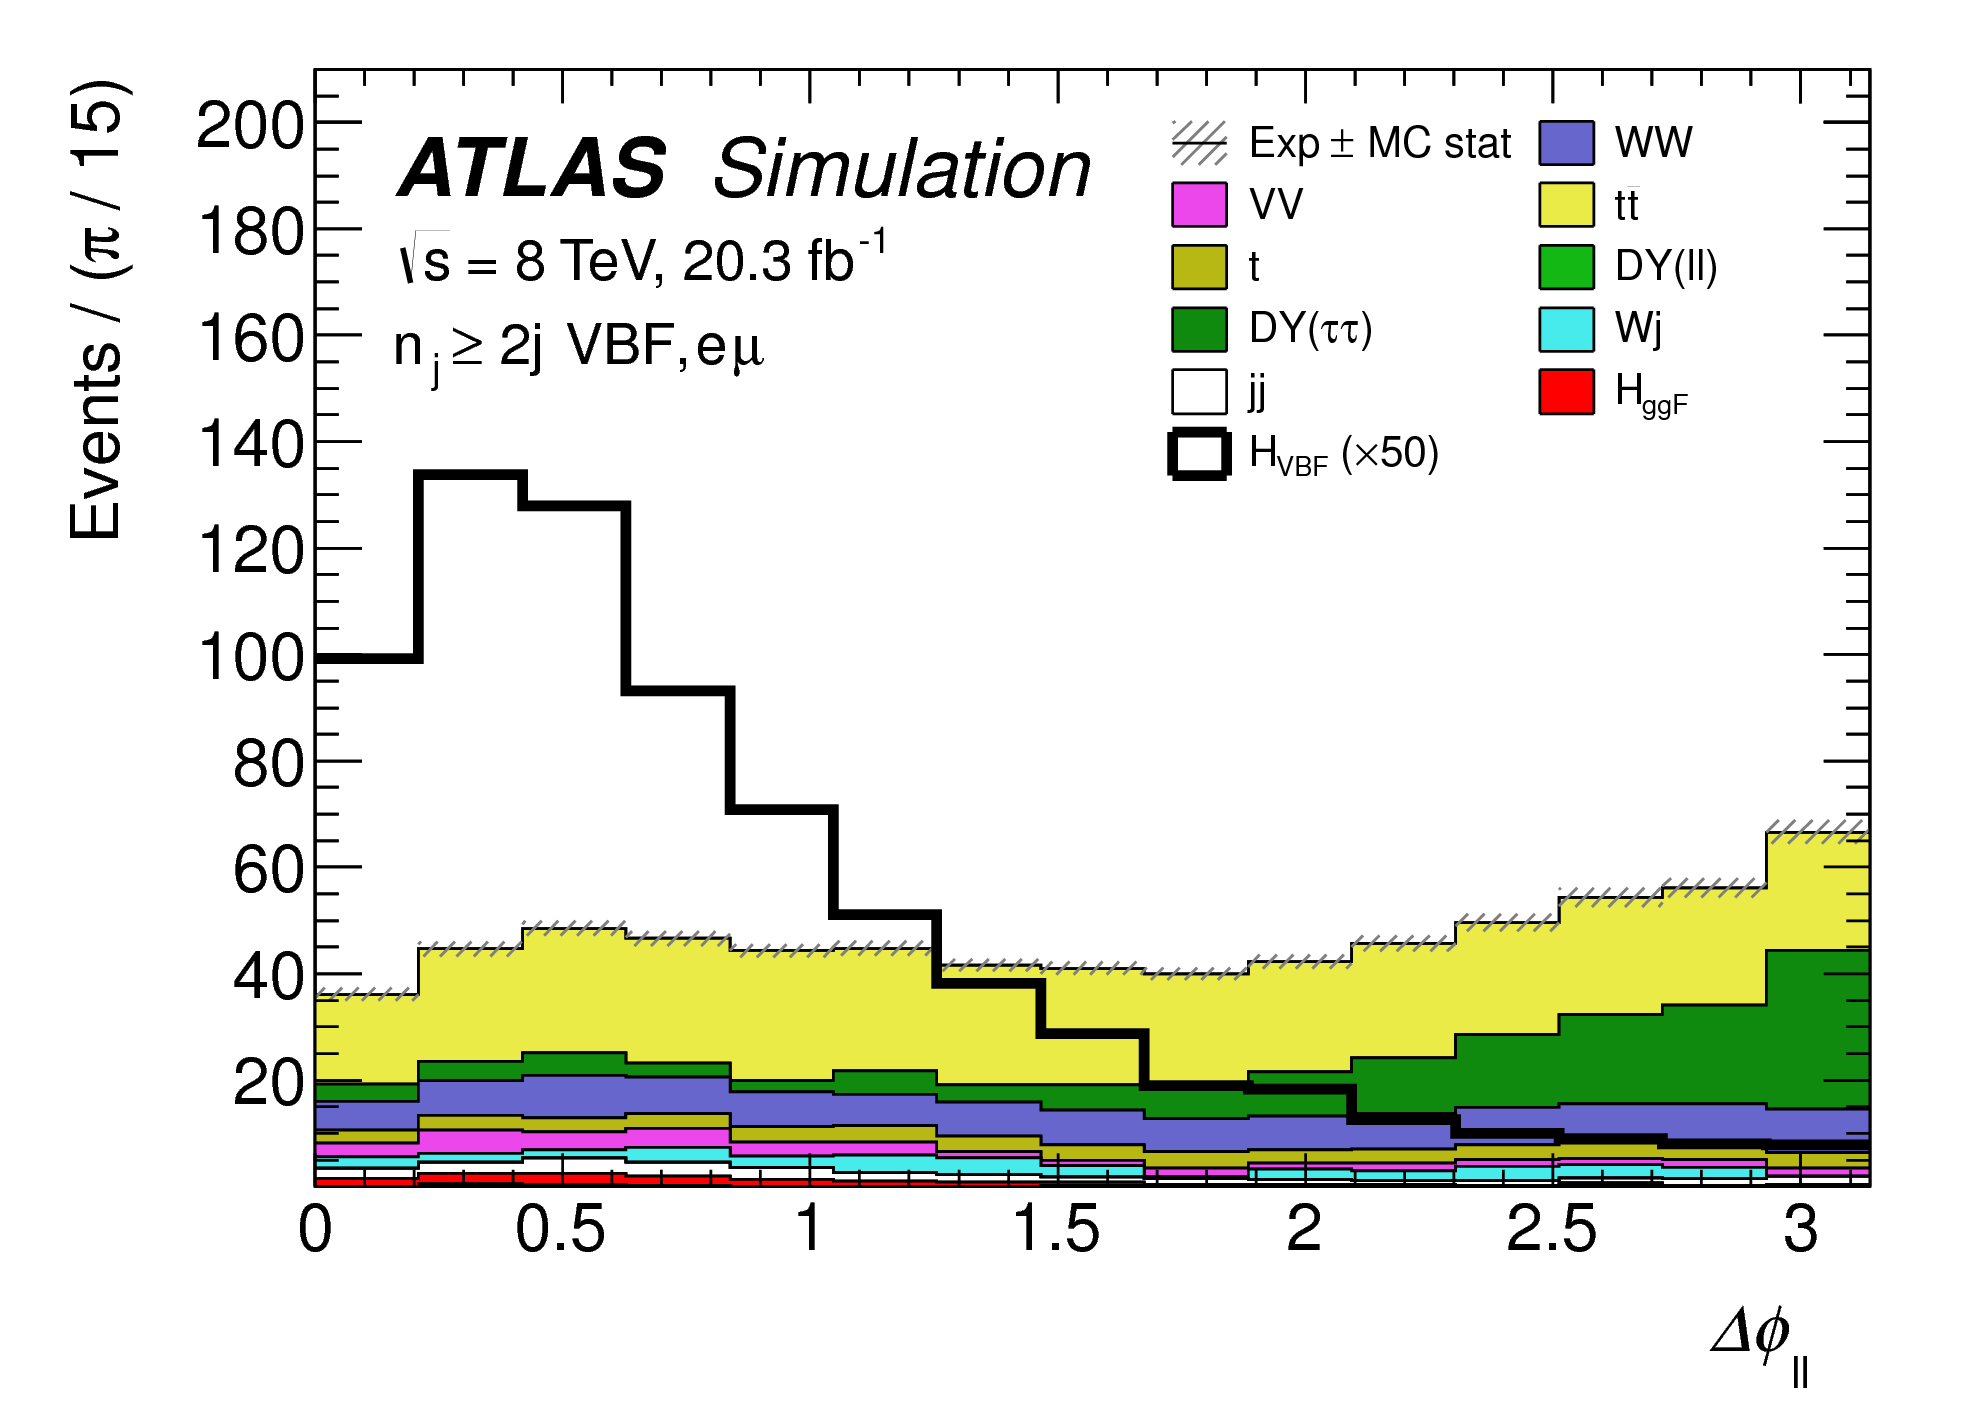
\includegraphics[width=0.45\textwidth]{figures/BDT_dphill}
  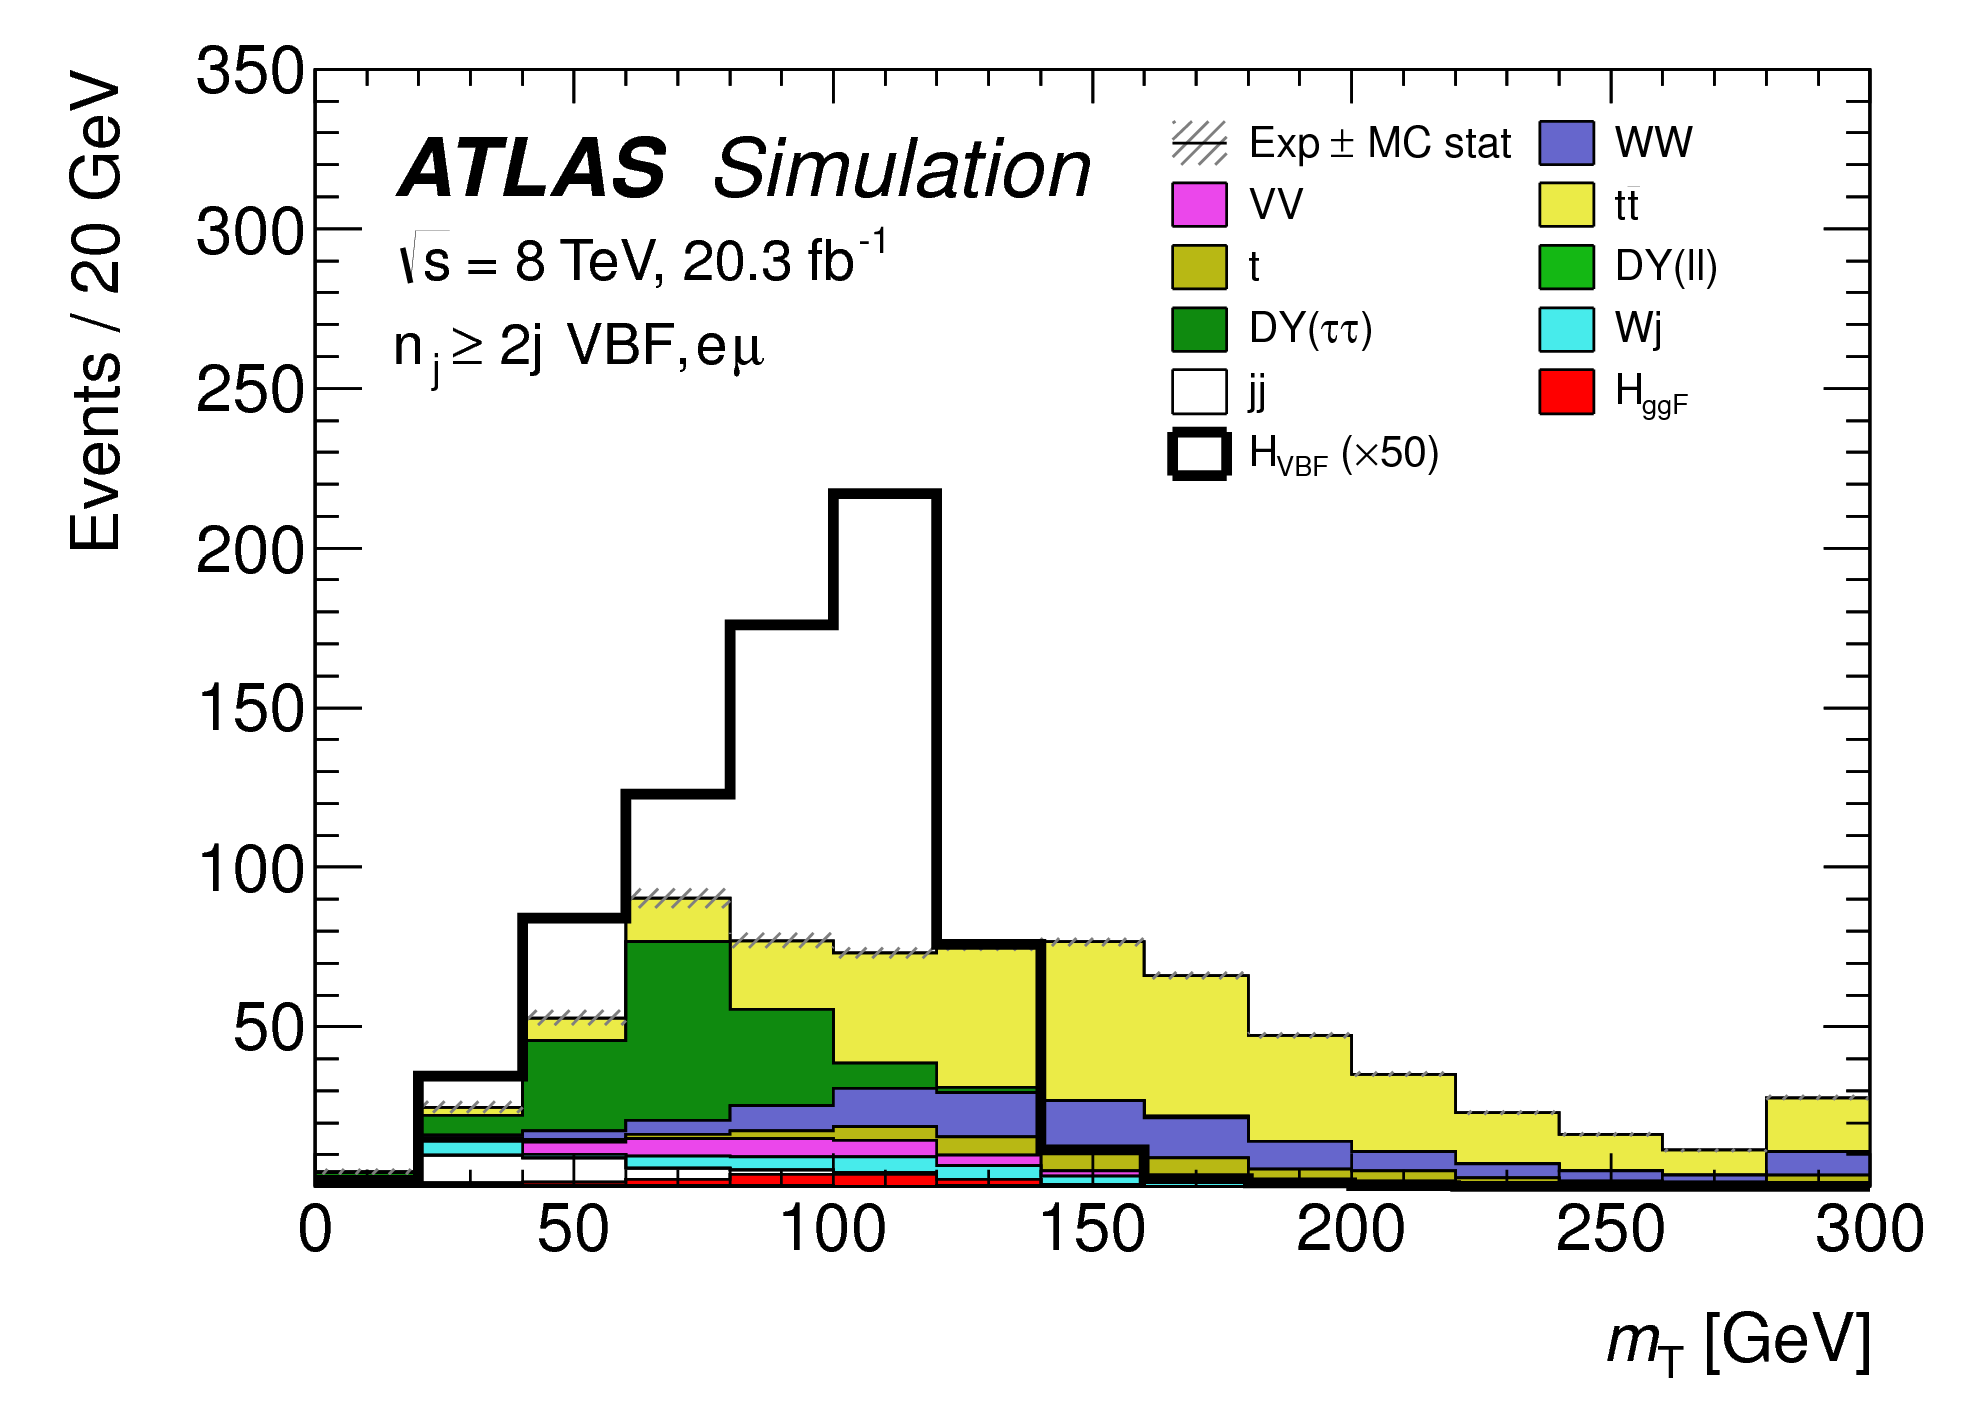
\includegraphics[width=0.45\textwidth]{figures/BDT_mT}

  \caption{Higgs topology variables - $\mll$ (top left), $\dphill$ (top right), and $\mTH$ (bottom) - used in the selection requirements of the cut-based signal region and as inputs to the BDT result. These are plotted after all of the BDT pre-training selection cuts~\cite{WW2015}. The VBF Higgs signal cross section is multiplied by a factor of $50$ to allow for shape comparisons.}
  \label{fig:vbf_bdt_htopo}
\end{figure}

\begin{figure}[h!]
  \centering
  \captionsetup{justification=centering}
  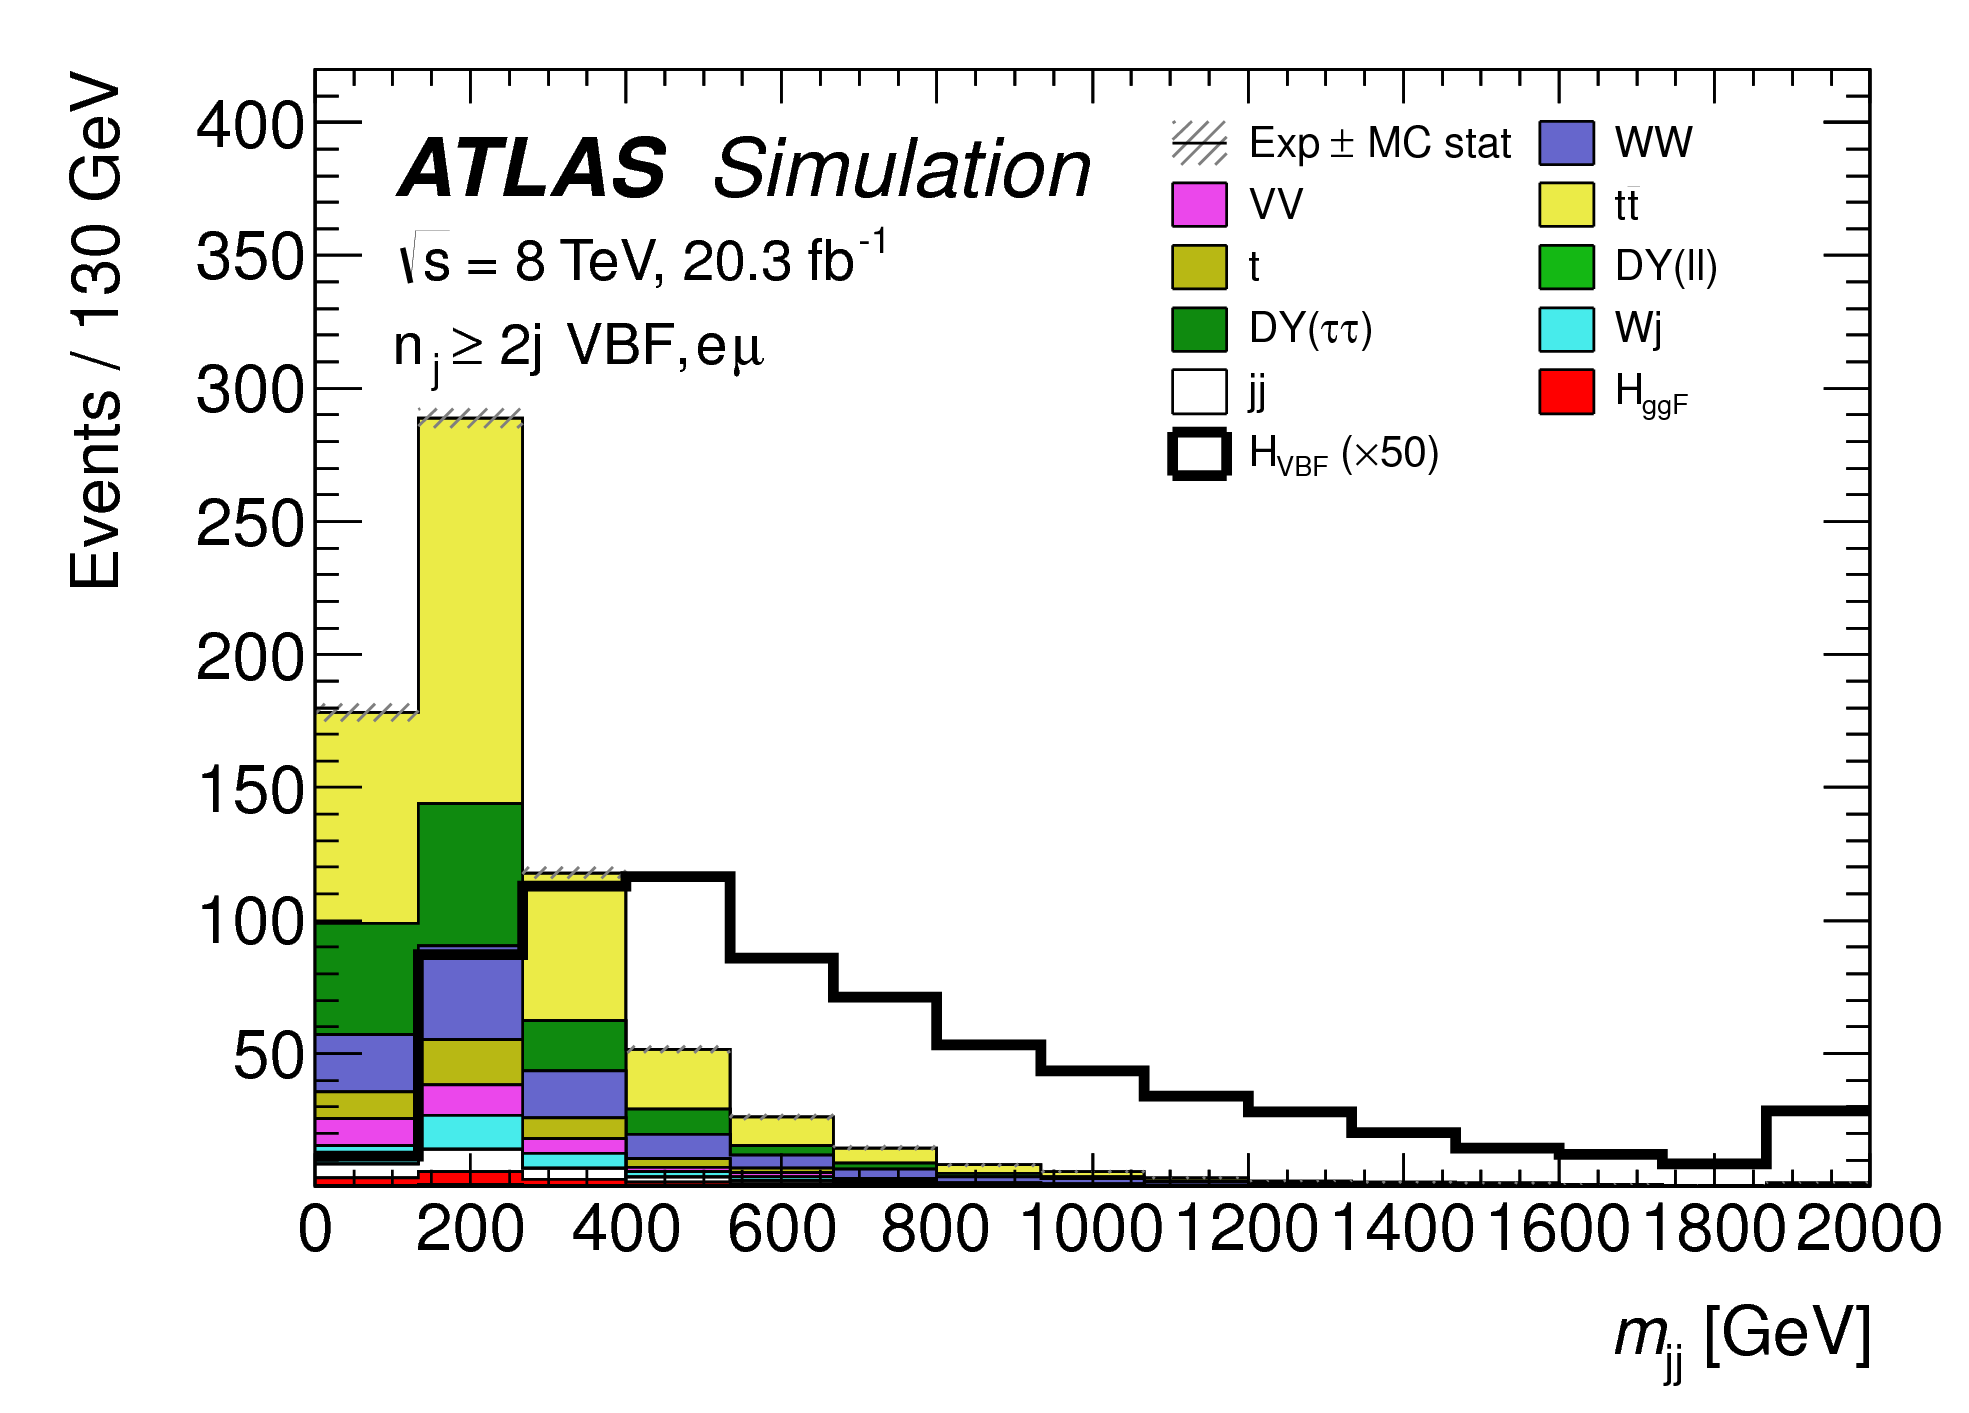
\includegraphics[width=0.45\textwidth]{figures/BDT_mjj}
  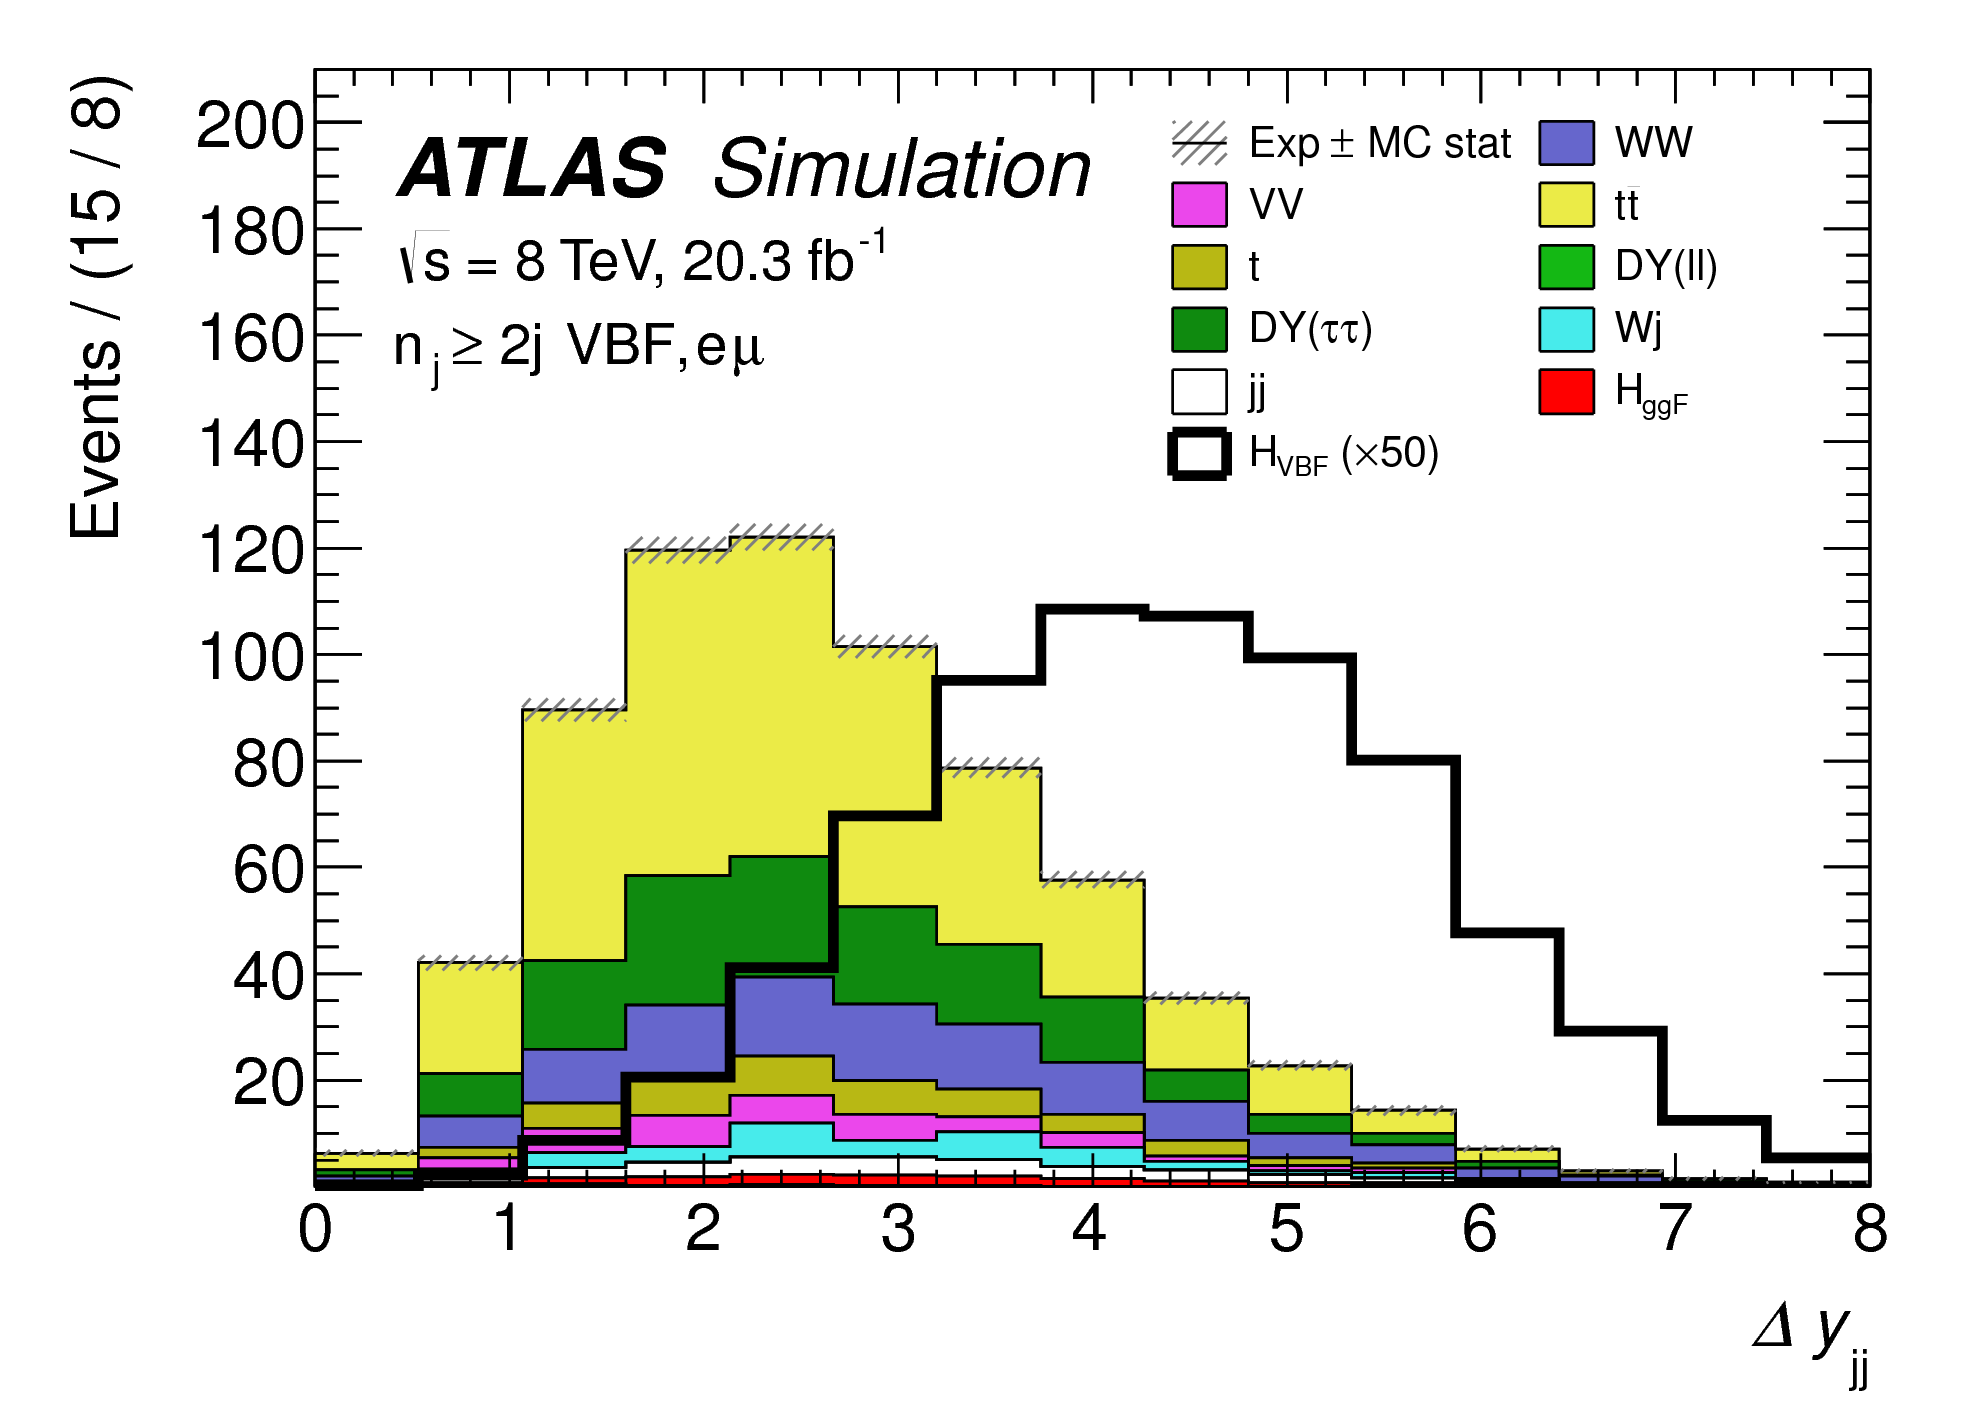
\includegraphics[width=0.45\textwidth]{figures/BDT_dyjj}
  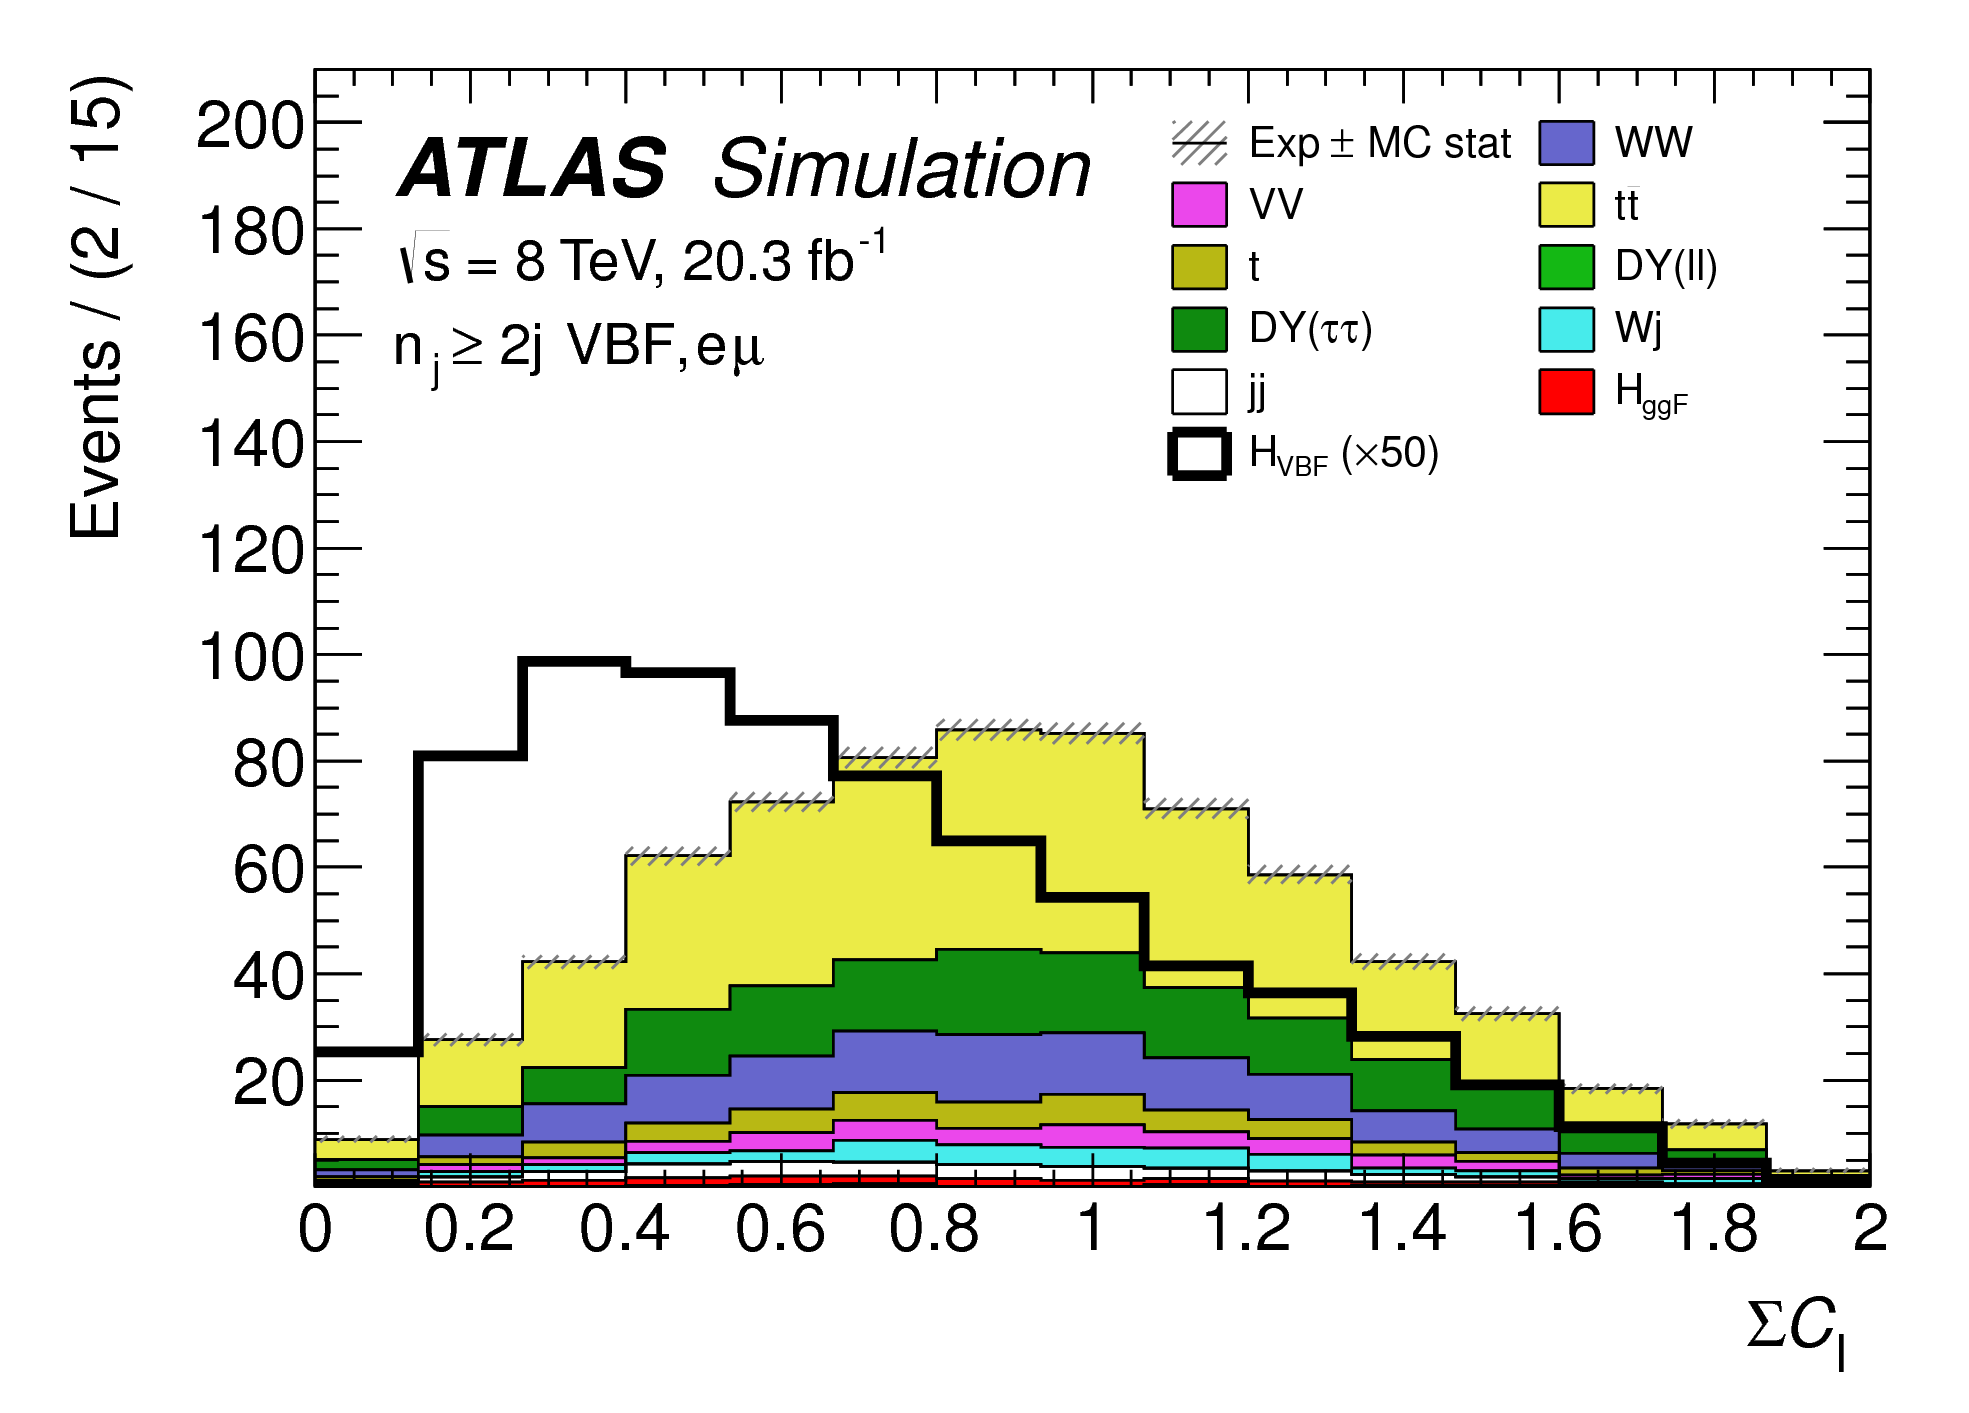
\includegraphics[width=0.45\textwidth]{figures/BDT_olv}
  \caption{VBF topology variables - $\mjj$ (top left), $\dyjj$ (top right), $\sum\olv$ (bottom) - used in the selection requirements of the cut-based signal region and as inputs to the BDT result. These are plotted after all of the BDT pre-training selection cuts~\cite{WW2015}. The VBF Higgs signal cross section is multiplied by a factor of $50$ to allow for shape comparisons.}
  \label{fig:vbf_bdt_vbftopo}
\end{figure}

%\begin{table}[h!]

%\begin{tabular}{|c|c|c|c|}
%\hline
% & Selection & Cut-based & BDT \\ \hline
%\multirow{7}{*}{Shared cuts} & Lepton & \multicolumn{2}{c|}{Two opposite charge leptons with $p_{T} > 22 (10) \GeV$} \\ \cline{2-4} 
%& $\mll$ & $> 10 (12) \GeV$ for $e\mu$ ($ee + \mu\mu$) \\ \cline{2-4}


%\hline
%\end{tabular}
%\caption{Summary of VBF selections for cut-based and BDT analyses}
%\label{tab:vbfcuts}
%\end{table}

%\subsubsection{BDT output}

%After training, the BDT outputs a score ($\bdt$) which is in the range $[-1, 1]$, where $-1$ corresponds to background-like events and $+1$ corresponds to signal-like events. Figure~\ref{fig:bdtscore} shows the output BDT distribution in both the different flavor and same flavor channels. For the final discriminant analysis, the $\bdt$ distribution is divided into four bins, with boundaries at $[-1, -0.48, -0.3, 0.78, 1]$. The bins are numbered from $0,1,2,3$ respectively. Because bin $0$ is predominantly background, it is excluded from the likelihood analysis. 

%\begin{figure}[h!]
%  \centering
%  \captionsetup{justification=centering}
%  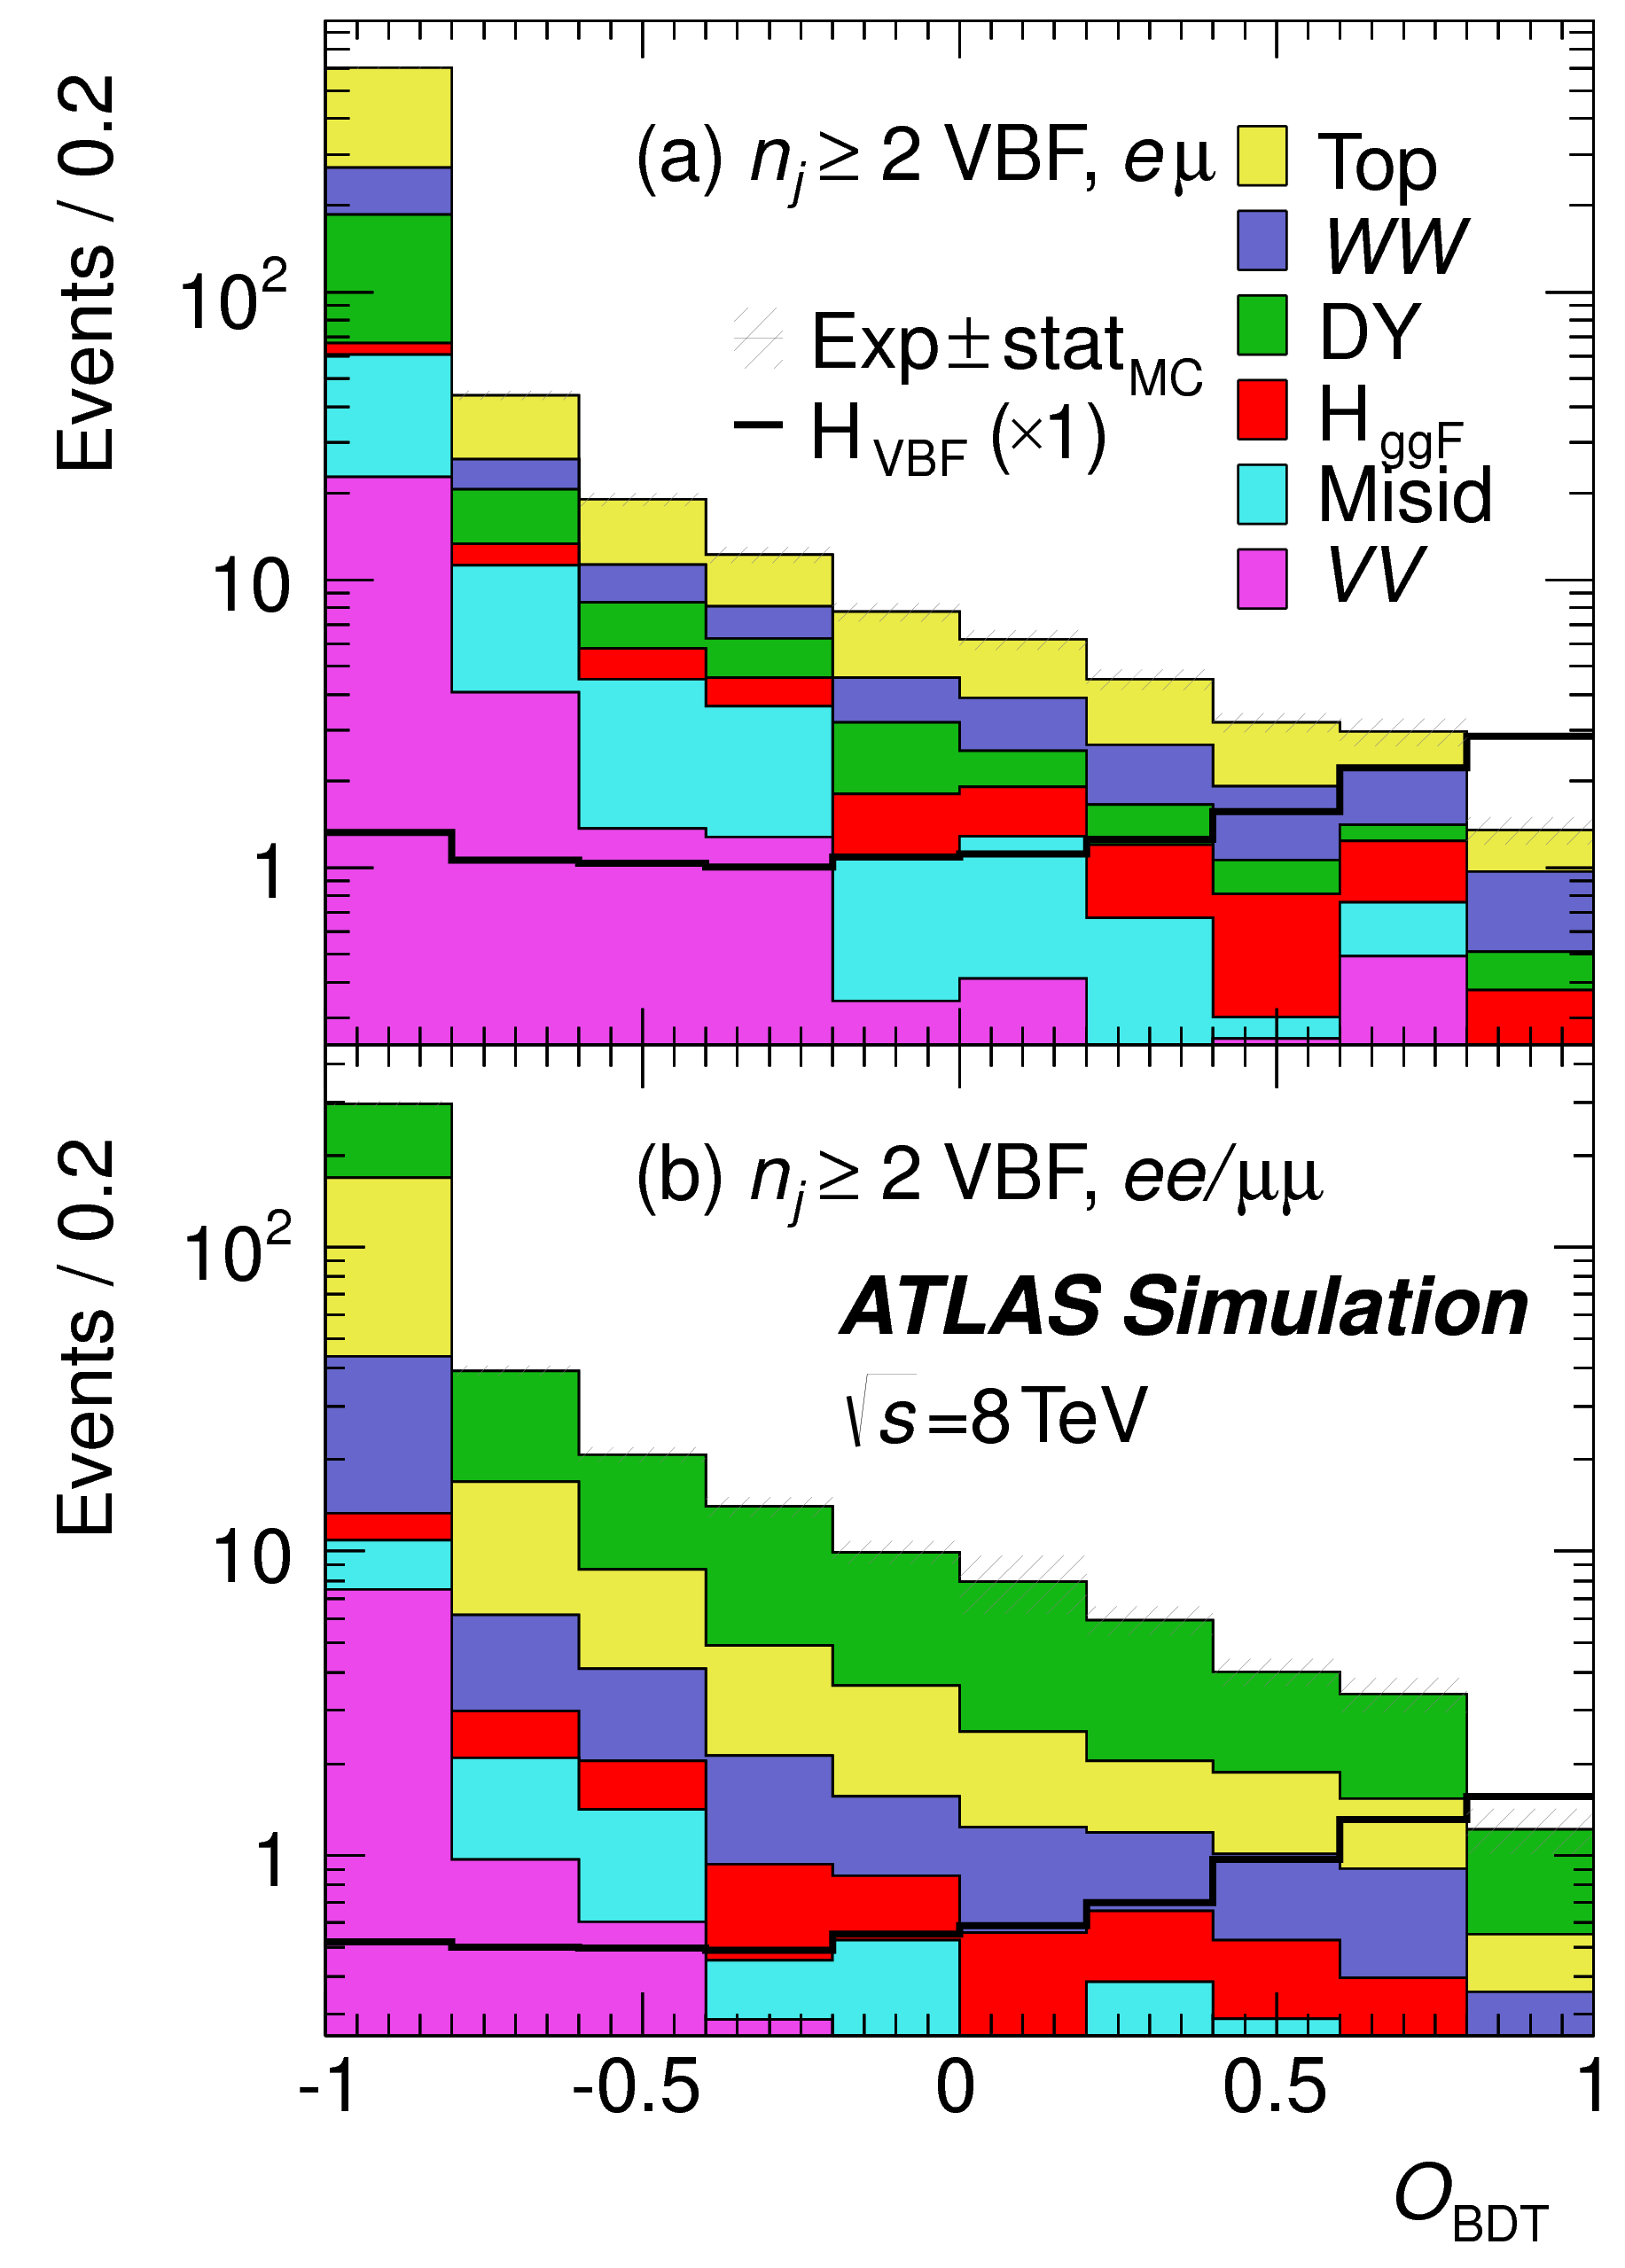
\includegraphics[width=0.6\textwidth]{figures/BDT_score}
%  \caption{Distributions of $\bdt$ for the VBF signal and associated backgrounds after the VBF pre-training selection\cite{WW2015}.}
%  \label{fig:bdtscore}
%\end{figure}

\section{Background estimation}
\label{sec:HWWbkg}

This section describes the procedures used to estimate backgrounds for the VBF analysis in both the cut-based and BDT analyses. First, the general strategy is presented. Then, specific procedures for each background in both signal regions are shown. 

\subsection{General strategy}

Most of the backgrounds in both the gluon fusion and VBF Higgs analyses have shapes estimated from Monte Carlo simulation but normalizations derived from control regions in data. In essence, a normalization factor (denoted with $\beta$ or abbreviated as NF) is derived by scaling the MC yield in the control region to the corresponding yield in data. Once this factor is derived, it can be used to scale the MC estimate of the background in the signal region. This is illustrated in equation~\ref{eqn:nf}.
%
\begin{equation}
B_{\rm SR}^{\rm est} = B_{\rm SR} \times \frac{N_{\rm CR}}{B_{\rm CR}} \equiv B_{\rm SR} \times \beta
\label{eqn:nf}
\end{equation}
%
Here, $B$ is the MC yield prediction in the denoted region, while $N$ is the observed number of events in data in the denoted region. 

There is an alternative way of writing the same equation in terms of an extrapolation factor $\alpha$ rather than a normalization factor $\beta$. The overall calculation is exactly the same. However, when phrased in this way, it shows how the uncertainty on the background estimation can be reduced. This is shown in equation~\ref{eqn:nf2}.
%
\begin{equation}
B_{\rm SR}^{\rm est} = N_{\rm CR} \times \frac{B_{\rm SR}}{B_{\rm CR}} \equiv N_{\rm CR} \times \alpha
\label{eqn:nf2}
\end{equation}
%
Phrased this way, the equation shows that with enough events in the control region, a large theoretical uncertainty on the overall background yield in the signal region can be replaced by a small statistical uncertainty coming from the number of data events in the CR and a smaller theoretical uncertainty on the extrapolation from the control region to the signal region. 

\subsection{Top background}
\label{sec:topnf}
The normalization factor $\beta_{t}$ for the top background in the VBF analysis is derived in a region required to have one $b$-tagged jet, or $\Nbjet = 1$. In the cut-based analysis, normalization factors are computed after every selection requirement by making the same requirements in the CR. These NF are then applied to the $\ttbar$ and single top event yields in the SR. In the BDT analysis, a single normalization factor is computed for each bin of $\bdt$ after applying the BDT pre-training cuts described previously. The computed normalization factors are derived with all flavor combinations combined in order to decrease statistical uncertainty. Additionally, in the BDT analysis, BDT bins 2 and 3 are merged for the same reason.

Table~\ref{tab:vbf_cb_topnf} shows the evolution of the $\beta_{t}$ through the cut-based selection. Table~\ref{tab:vbf_bdt_topnf} shows the value of the $\beta_{t}$ in each bin of $\bdt$. The computed factors are almost all relatively consistent with unity, except for bin $1$ of $\bdt$ which requires a larger correction. The normalization factors in bins 2 and 3 of $\bdt$ are also consistent with those derived in the cut-based signal region, increasing confidence in the BDT estimation. 
%
\begin{table}[h!]
\centering
\captionsetup{justification=centering}
\begin{tabular}{|c|c|}
\hline
Cut & $\beta_t$ \\ \hline
$\pTtot < 15 \GeV$ & $1.03 \pm 0.01$ \\ \hline
$\mtt < m_Z - 25$ & $1.05 \pm 0.01$ \\ \hline
$\mjj > 600 \GeV$ & $0.96 \pm 0.06$ \\ \hline
$\dyjj > 3.6 $ & $1.02 \pm 0.08$ \\ \hline
$\rm CJV$ & $1.13 \pm 0.16$ \\ \hline
$\rm OLV$ & $1.01 \pm 0.19$ \\ \hline
$\mjj < 1 \TeV$ & $0.94 \pm 0.19$ \\ \hline
$\mjj > 1 \TeV$ & $1.48 \pm 0.66$ \\ \hline 
\end{tabular}
\caption{Top normalization factors computed at each stage of the cut-based selection. Uncertainties are statistical only.}
\label{tab:vbf_cb_topnf}
\end{table}
%
\begin{table}[h!]
\centering
\captionsetup{justification=centering}
\begin{tabular}{|c|c|}
\hline
$\bdt$ & $\beta_t$ \\ \hline
Bin $0$ & $1.09 \pm 0.02$ \\ \hline
Bin $1$ & $1.58 \pm 0.15$ \\ \hline
Bin $2$ & $0.95 \pm 0.31$ \\ \hline
Bin $3$ & $0.95 \pm 0.31$ \\ \hline
\end{tabular}
\caption{Top normalization factors computed for each bin of $\bdt$. Uncertainties are statistical only.}
\label{tab:vbf_bdt_topnf}
\end{table}
%
Figure~\ref{fig:vbf_top_cr} shows the $\mjj$ and $\bdt$ distributions in the top control region. Overall the modeling looks consistent with the data.
While these normalization factors can be computed and applied to the expected background yields listed in tables like table~\ref{tab:vbf_cutflow_bkg}, the final normalization of the top background is profiled (meaning there is a dedicated Poisson constraint) and allowed to float in the final statistical fit. 

\begin{figure}[h!]
  \centering
  \captionsetup{justification=centering}
  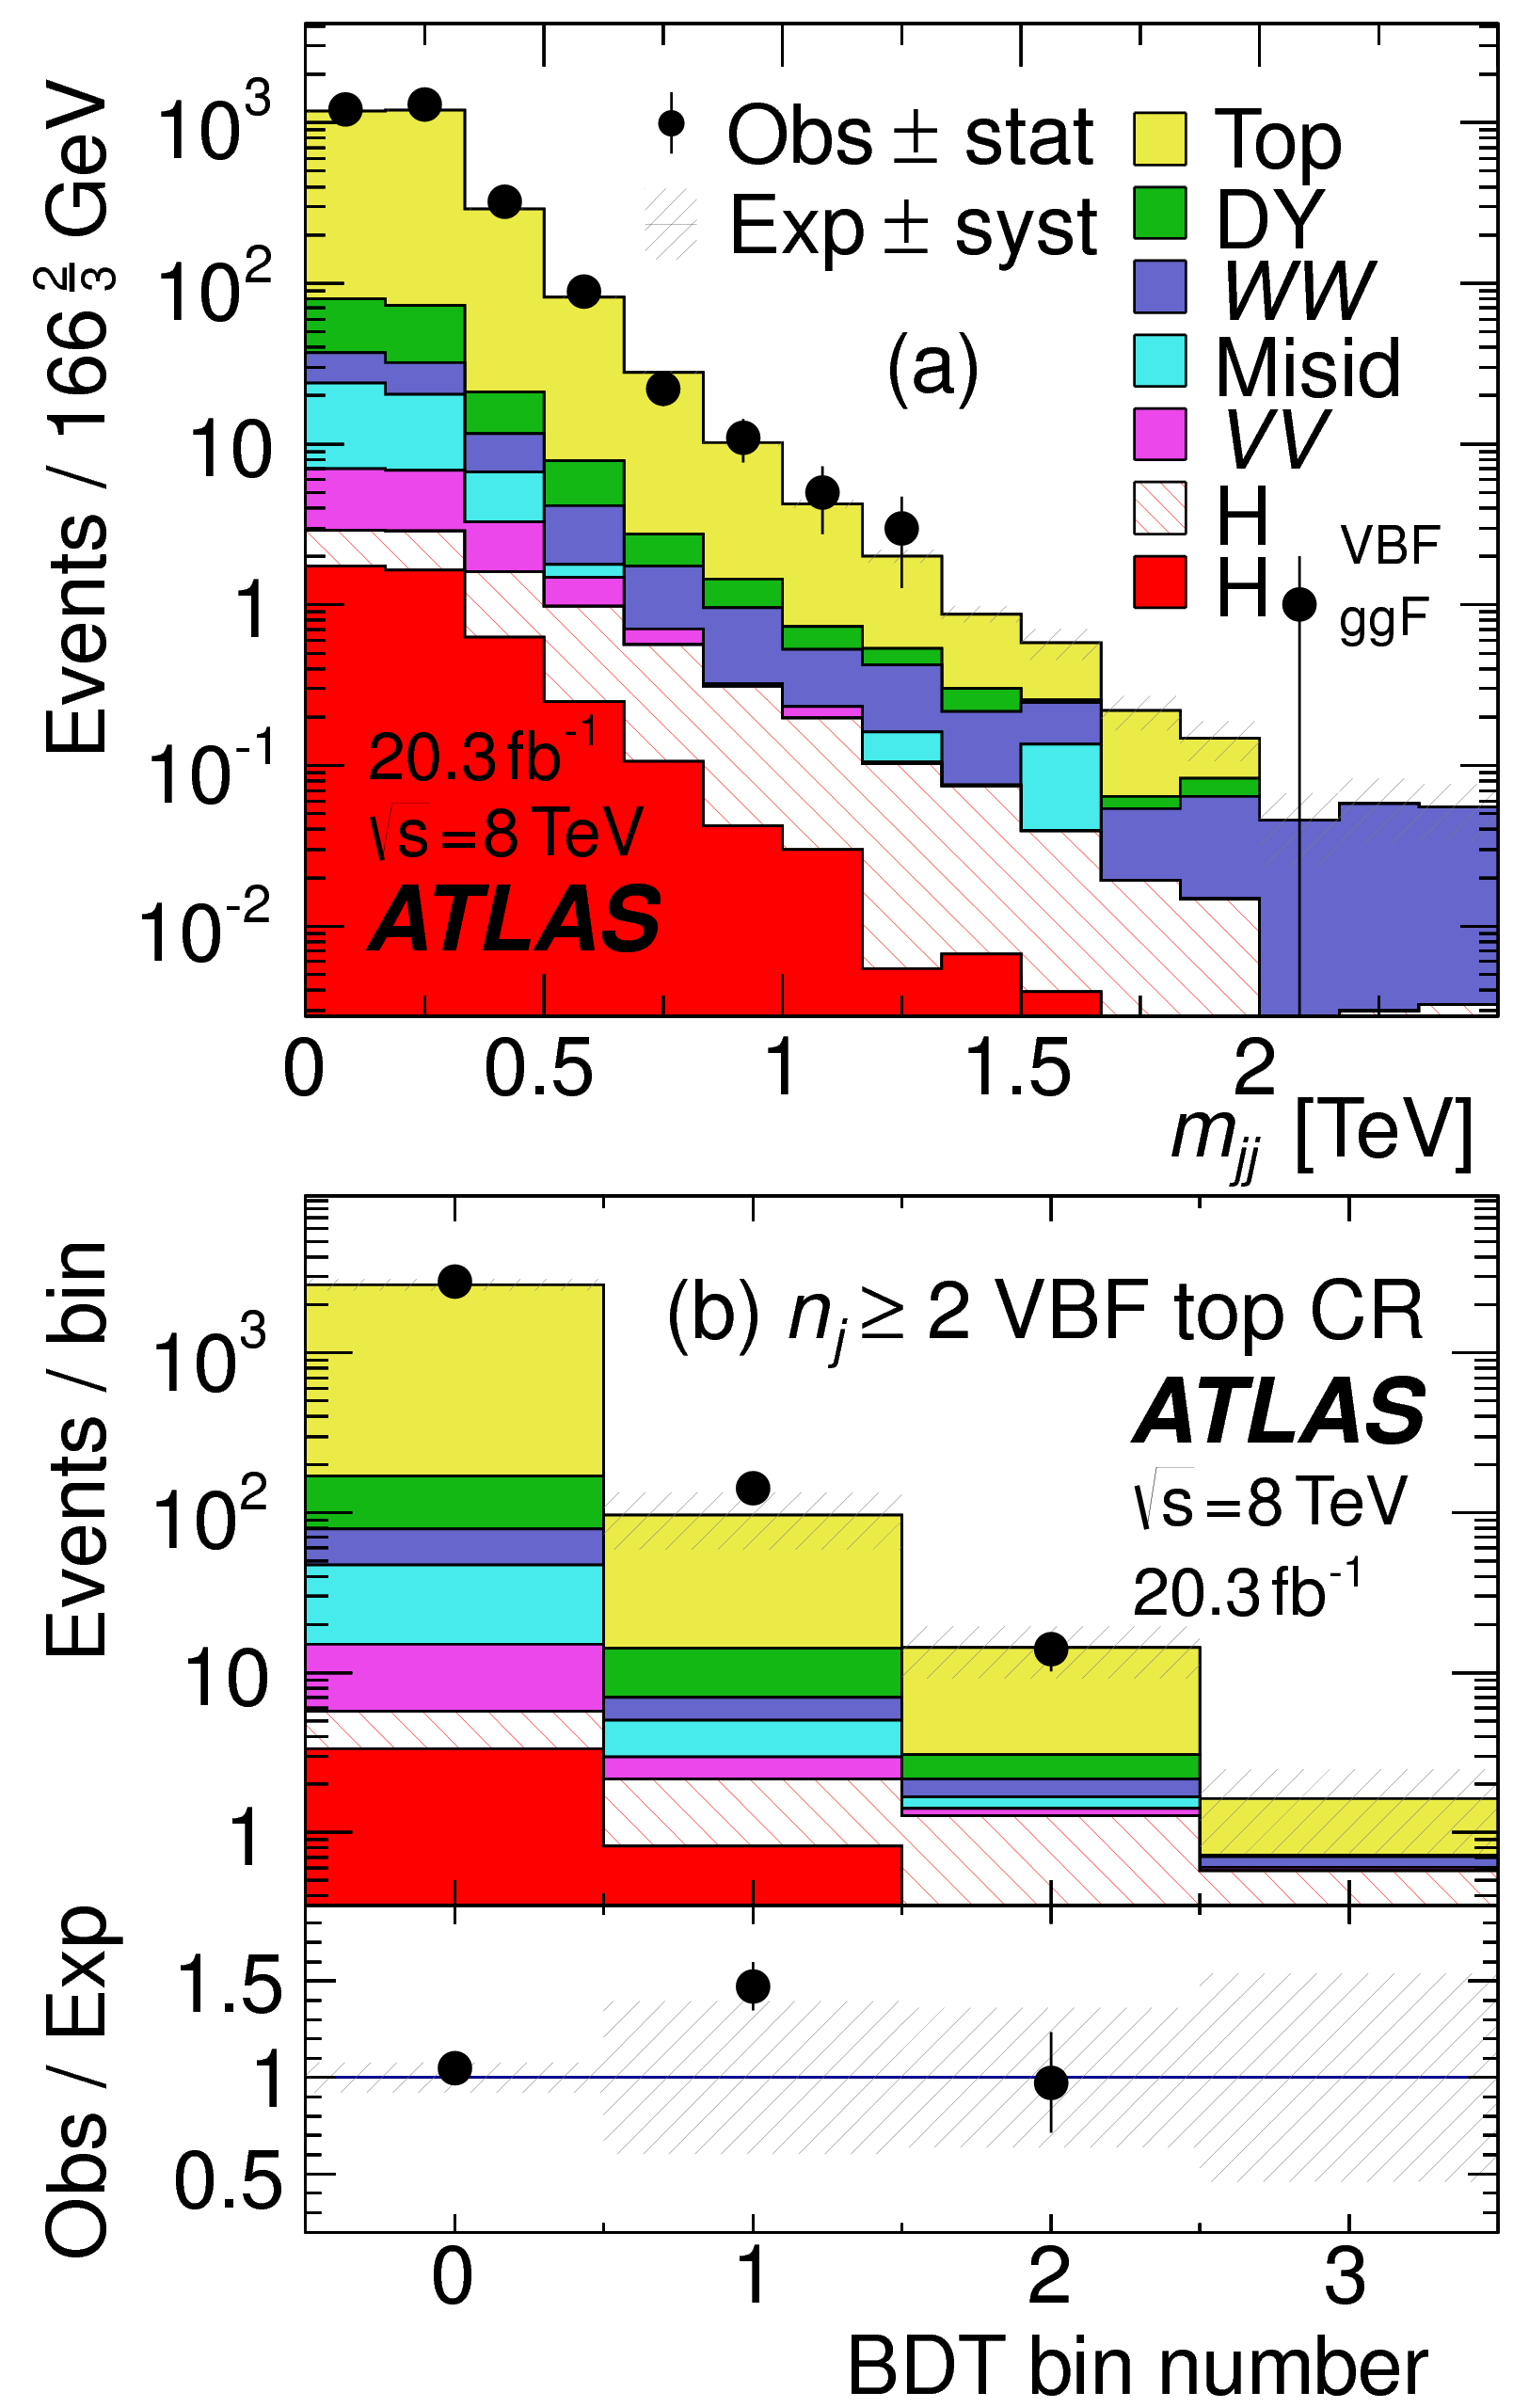
\includegraphics[width=0.5\textwidth]{figures/VBF_topcr}
  \caption{Distributions of $\mjj$ (a) and $\bdt$ (b) in the VBF $\Nbjet = 1$ top CR~\cite{WW2015}.}
  \label{fig:vbf_top_cr}
\end{figure}

\subsection{$\ZDY \to \tau\tau$ background}

In the different flavor channels, the $\ZDY \to \tau\tau$ background is an important one. Di-tau production can produce an $e\mu$ final state if each $\tau$ lepton decays to a different flavor lepton. 

In the BDT analysis, a single normalization factor for the background is derived. A control region is defined using the pre-training selection cuts, except requiring that $|\mtt - m_Z| < 25 \GeV$ so that the region is enriched in $\ZDY \to \tau\tau$ background. Additional requirements of $\mll < 80 (75) \GeV$ in the different (same) flavor channel, as well as $\bdt > -0.48$ are applied to increase the purity of the region. The final $\beta_{\ZDY \to \tau\tau}$ is calculated to be $0.9 \pm 0.3$ (statistical uncertainty only). Because of the small contribution of this background in the BDT analysis and the large statistical uncertainty, no additional systematics are calculated. The final SR estimate is scaled by this $\beta$ and not allowed to float in the fit. 

The cut-based corrections are a bit more involved because they need to be applied selection by selection, as well as in the final signal region for the fit. The control region is defined including all SR requirements up to the $\ZDY \to \tau\tau$ veto, which is instead turned into a Z mass peak requirement as for the BDT region. The $\mll$ cut from the BDT region is included as well. The cut-based approach aims to correct the normalization of the $\ZDY \to\tau\tau$ background in two ways. First, an overall normalization factor is computed from the control region. However, the VBF topological cuts are not included in this region, and applying them as is done in the top CR is not feasible due to limited statistics. So, instead, correction factors (CF) to the cut efficiencies of the VBF cuts are derived in a same flavor $Z\to\ell\ell$ control region, which has significantly more statistics. The CF is simply the ratio of the cut efficiencies in data and MC derived in this region. In the end, the overall background estimate is given by equation~\ref{eqn:zttest}.
%
\begin{equation}
N^{\rm est}_{\ZDY \to \tau\tau} = B^{\rm SR}_{\ZDY \to \tau\tau} \times \beta_{\tau\tau} \times \frac{\epsilon_{\rm VBF\,cuts}^{\rm data}}{\epsilon_{\rm VBF\,cuts}^{\rm MC}} 
\label{eqn:zttest}
\end{equation}
%
The hypothesis is that while the normalization correction must be derived in a dedicated region, the efficiency of the VBF topology requirements should not be sensitive to the type of $\ZDY$ process and thus the higher number of events can be exploited to derive the CF. Figure~\ref{fig:vbf_ztt_comp} shows a shape comparison for the $\mjj$ variable in $Z\to\tau\tau$ events in the signal region and $Z\to\ell\ell$ events in the control region. The figure shows that the shapes are indeed comparable and thus any CF derived in the same flavor control region can reliably be applied in the signal region. 

\begin{figure}[h!]
  \centering
  \captionsetup{justification=centering}
  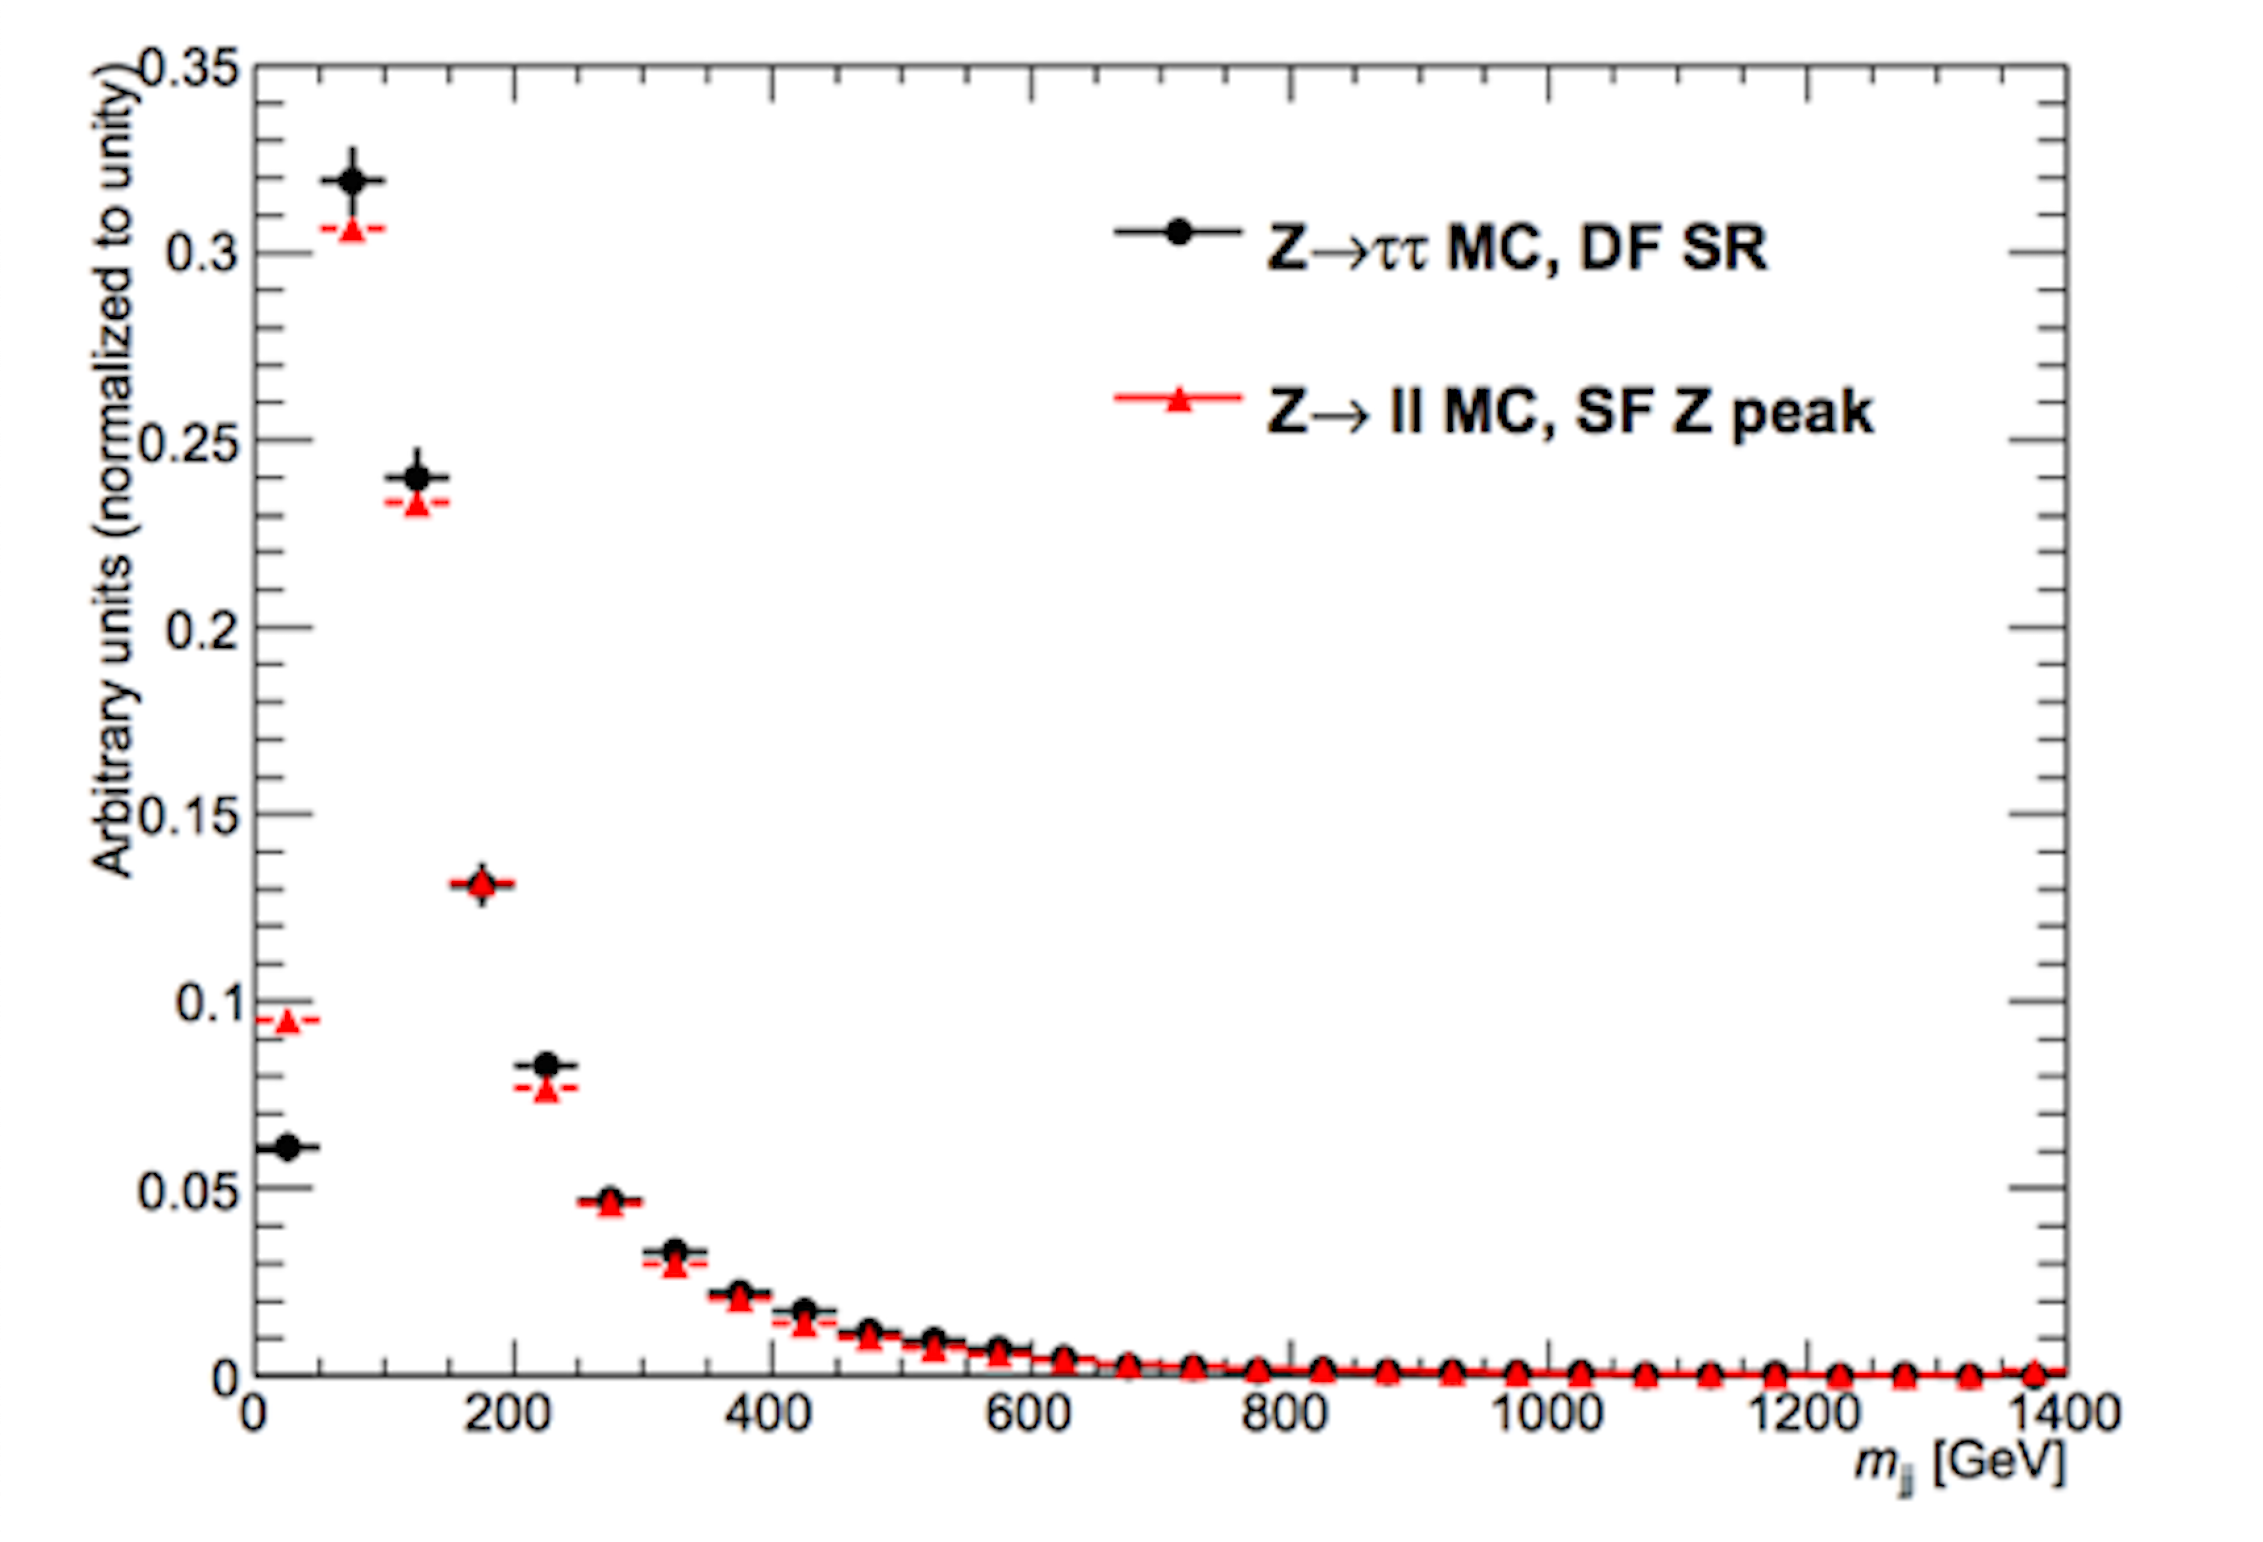
\includegraphics[width=0.6\textwidth]{figures/VBF_DYtt_shape_comp}
  \caption{Comparison of $\mjj$ shape in a same flavor $Z\to\ell\ell$ control region and the VBF cut-based signal region. The MC samples used for these distributions are given in table~\ref{tab:HWW-MC}.}
  \label{fig:vbf_ztt_comp}
\end{figure}

Table~\ref{tab:vbf_cb_zttnf} shows the overall normalization factor $\beta_{\tau\tau}$ and the efficiency correction factors for the various VBF topological cuts. In general, the statistical uncertainties on the cut efficiency corrections are quite good, and the MC tends to underestimate the efficiency of the VBF cuts for the $\ZDY\to\tau\tau$ background. The overall normalization factor is also consistent with that calculated for the BDT analysis.

\begin{table}[h!]
\centering
\captionsetup{justification=centering}
\begin{tabular}{|c|c|}
\hline
$\beta_{\tau\tau}$ & $0.97 \pm 0.04$ \\ \hline\hline
 Cut & Correction factors (CF) \\ \hline
$\mjj > 600 \GeV$ & $1.09 \pm 0.01$ \\ \hline
$\dyjj > 3.6 $ & $1.14 \pm 0.02$ \\ \hline
$\rm CJV$ & $1.20 \pm 0.02$ \\ \hline
$\rm OLV$ & $1.17 \pm 0.03$ \\ \hline
$\mjj < 1 \TeV$ & $1.17 \pm 0.06$ \\ \hline
$\mjj > 1 \TeV$ & $1.18 \pm 0.13$ \\ \hline 
\end{tabular}
\caption{$\ZDY \to\tau\tau$ correction factors for the VBF cut-based analysis. Uncertainties are statistical only.}
\label{tab:vbf_cb_zttnf}
\end{table}

\subsection{$\ZDY \to \ell\ell$ background}

In the same flavor channels, the $\ZDY \to \ell\ell$ background is dominant and thus must be estimated correctly. In both the BDT and cut-based analyses, the background is estimated using the so-called ``ABCD" method. The ABCD method creates four different regions by defining requirements on two variables. One of the regions (A) is the signal region, while the other regions are defined by inverting one of both of the requirements. in this case, the two variables used are $\mll$ and $\MET$, because inverting either of the SR cuts on these variables will give regions rich in the $\ZDY\to\ell\ell$ background. Figure~\ref{fig:ABCDcuts} illustrates the definitions of each region. 


%\begin{table}[h!]
%\centering
%\captionsetup{justification=centering}
%\begin{tabular}{|c|c|}
%\specialcell{$\rm \mathbf{Region A (SR)}$ \\ High $\MET$ \\ Low $\mll$} & \specialcell{\textbf{Region C} \\ High $\MET$ \\ Z peak} \\ \hline
%\specialcell{\textbf{Region B} \\ Low $\MET$ \\ Low $\mll$} & \specialcell{\textbf{Region D} \\ Low $\MET$ \\ Z peak} \\ \hline
%\end{tabular}
%\caption{Illustration of the ABCD regions for $\ZDY \to\ell\ell$ background estimation.}
%\label{tab:ABCDcuts}
%\end{table}

\begin{figure}[h!]
  \centering
  \captionsetup{justification=centering}
  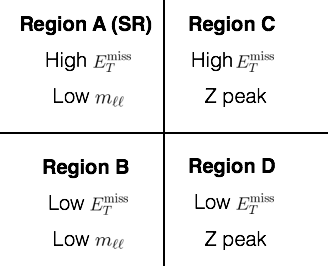
\includegraphics[width=0.4\textwidth]{figures/ABCD}
  \caption{General illustration of the ABCD region definitions for $\ZDY\to\ell\ell$ background estimation.}
  \label{fig:ABCDcuts}
\end{figure}

In both of the cut-based and BDT analyses, the Z peak region is defined with $|\mll - m_Z| < 15 \GeV$. In the cut-based analysis, low $\mll$ corresponds to $\mll < 50 \GeV$ (this defines the cut-based SR) while in the BDT it is $\mll < 75 \GeV$. In the cut-based, high and low $\MET$ are defined as opposite ends of the $55 \GeV$ cut applied for the signal region definition. The BDT low $\MET$ region is between $25$ and $45 \GeV$, while the high $\MET$ region is $\MET > 45 \GeV$. 

Once the regions are defined, the background in the signal region is estimated by extrapolating the estimate in region B to region A. This extrapolation is done by multiplying the number of events in region B by the ratio of the number of events in regions C and D. Effectively, the $Z$ peak region is used to estimate the efficiency of the $\MET$ requirement in data, and then this efficiency is applied in the low $\mll$ region. The method assumes that the $\MET$ efficiency is uncorrelated with $\mll$. The method can be applied in MC as a check on this assumption, and an additional correction, $f_{\rm corr}$, is applied for the non-closure of the method in MC. This is summarized in equations~\ref{eqn:abcd} and~\ref{eqn:nonclosure}.
%
\begin{equation}
N^{\rm SR}_{\ZDY\to\ell\ell} = N^{\rm B}_{\ZDY\to\ell\ell}  \times \frac{N^{\rm C}_{\ZDY\to\ell\ell}}{N^{\rm D}_{\ZDY\to\ell\ell} } \times f_{\rm corr}
\label{eqn:abcd}
\end{equation}
%
\begin{equation}
f_{\rm corr} = \frac{B_{\rm MC}^{\rm A}/B_{\rm MC}^{\rm B}}{B_{\rm MC}^{\rm C}/B_{\rm MC}^{\rm D}}
\label{eqn:nonclosure}
\end{equation}
%
Here, the $N$ refer to data yields in each region with the non $\ZDY$ backgrounds subtracted, while $B$ refer to the $\ZDY$ yields in MC in each region.

A normalization factor $\beta_{\ell\ell}$ is computed for each analysis as the ratio of the predicted data yield to the MC yield in the SR. The shape of the BDT distribution is taken from data region B, while the shape of the $\mTH$ distribution in the cut-based analysis is taken from $\ZDY$ MC in the SR. The values of $\beta_{\ell\ell}$ in the cut-based and BDT analyses from this method are summarized in table~\ref{tab:vbf_sf_nf}. They are quite consistent with one another within the statistical uncertainties. The value of $f_{\rm corr}$ is found to be $0.77\pm 0.13$. In the cut-based analysis, the same cut efficiency correction factors shown in table~\ref{tab:vbf_cb_zttnf} are also applied (in product with the $\beta_{\ell\ell}$) to obtain the final estimate of the $\ZDY$ background in the same flavor channels. 

\begin{table}[h!]
\centering
\captionsetup{justification=centering}
\begin{tabular}{|c|c|}
\hline
& $\beta_{\ell\ell}$ \\ \hline
$\rm BDT\,Bin\,1$ & $1.01 \pm 0.15$ \\ \hline
$\rm BDT\,Bin\,2$ & $0.89 \pm 0.28$ \\ \hline
$\rm Cut$-$\rm based$ & $0.81 \pm 0.21$ \\ \hline
\end{tabular}
\caption{$\ZDY \to \ell\ell$ normalization factors for cut-based and BDT analyses. Uncertainties are statistical only.}
\label{tab:vbf_sf_nf}
\end{table}

\subsection{$WW$ and other diboson backgrounds}

The Standard Model $WW$ and other diboson backgrounds ($WZ$, $ZZ$, $W\gamma$, $W\gamma^{*}$, and $Z\gamma$) have both their shape and normalization taken from MC simulation as they are subdominant in the VBF analysis. They are validated in dedicated control regions and found to agree with data well.

As SM $WW$ production is the largest of these backgrounds and is irreducible, validating the estimate is of particular importance. A validation region is constructed by requiring the pre-selection requirements on leptons and $\mll$, $\Nbjet = 0$, and $\mTH > 100 \GeV$. The $\mTtwo$ variable is an additional discriminant that has been shown to have to the ability to isolate the SM $WW$ background~\cite{mt2}. It is calculated by scanning over all possible values of neutrino momentum for both $W$ bosons and taking the minimum result. A requirement of $\mTtwo > 160 \GeV$ is placed to define the $WW$ validation region. This requirement gives a $60$\% purity for the validation region. The derived normalization factor in this region is $1.15 \pm 0.19$ and is thus consistent with unity. Figure~\ref{fig:mt2} shows the $\mTtwo$ distribution and how it distinguishes the $WW$ background.

\begin{figure}[h!]
  \centering
  \captionsetup{justification=centering}
  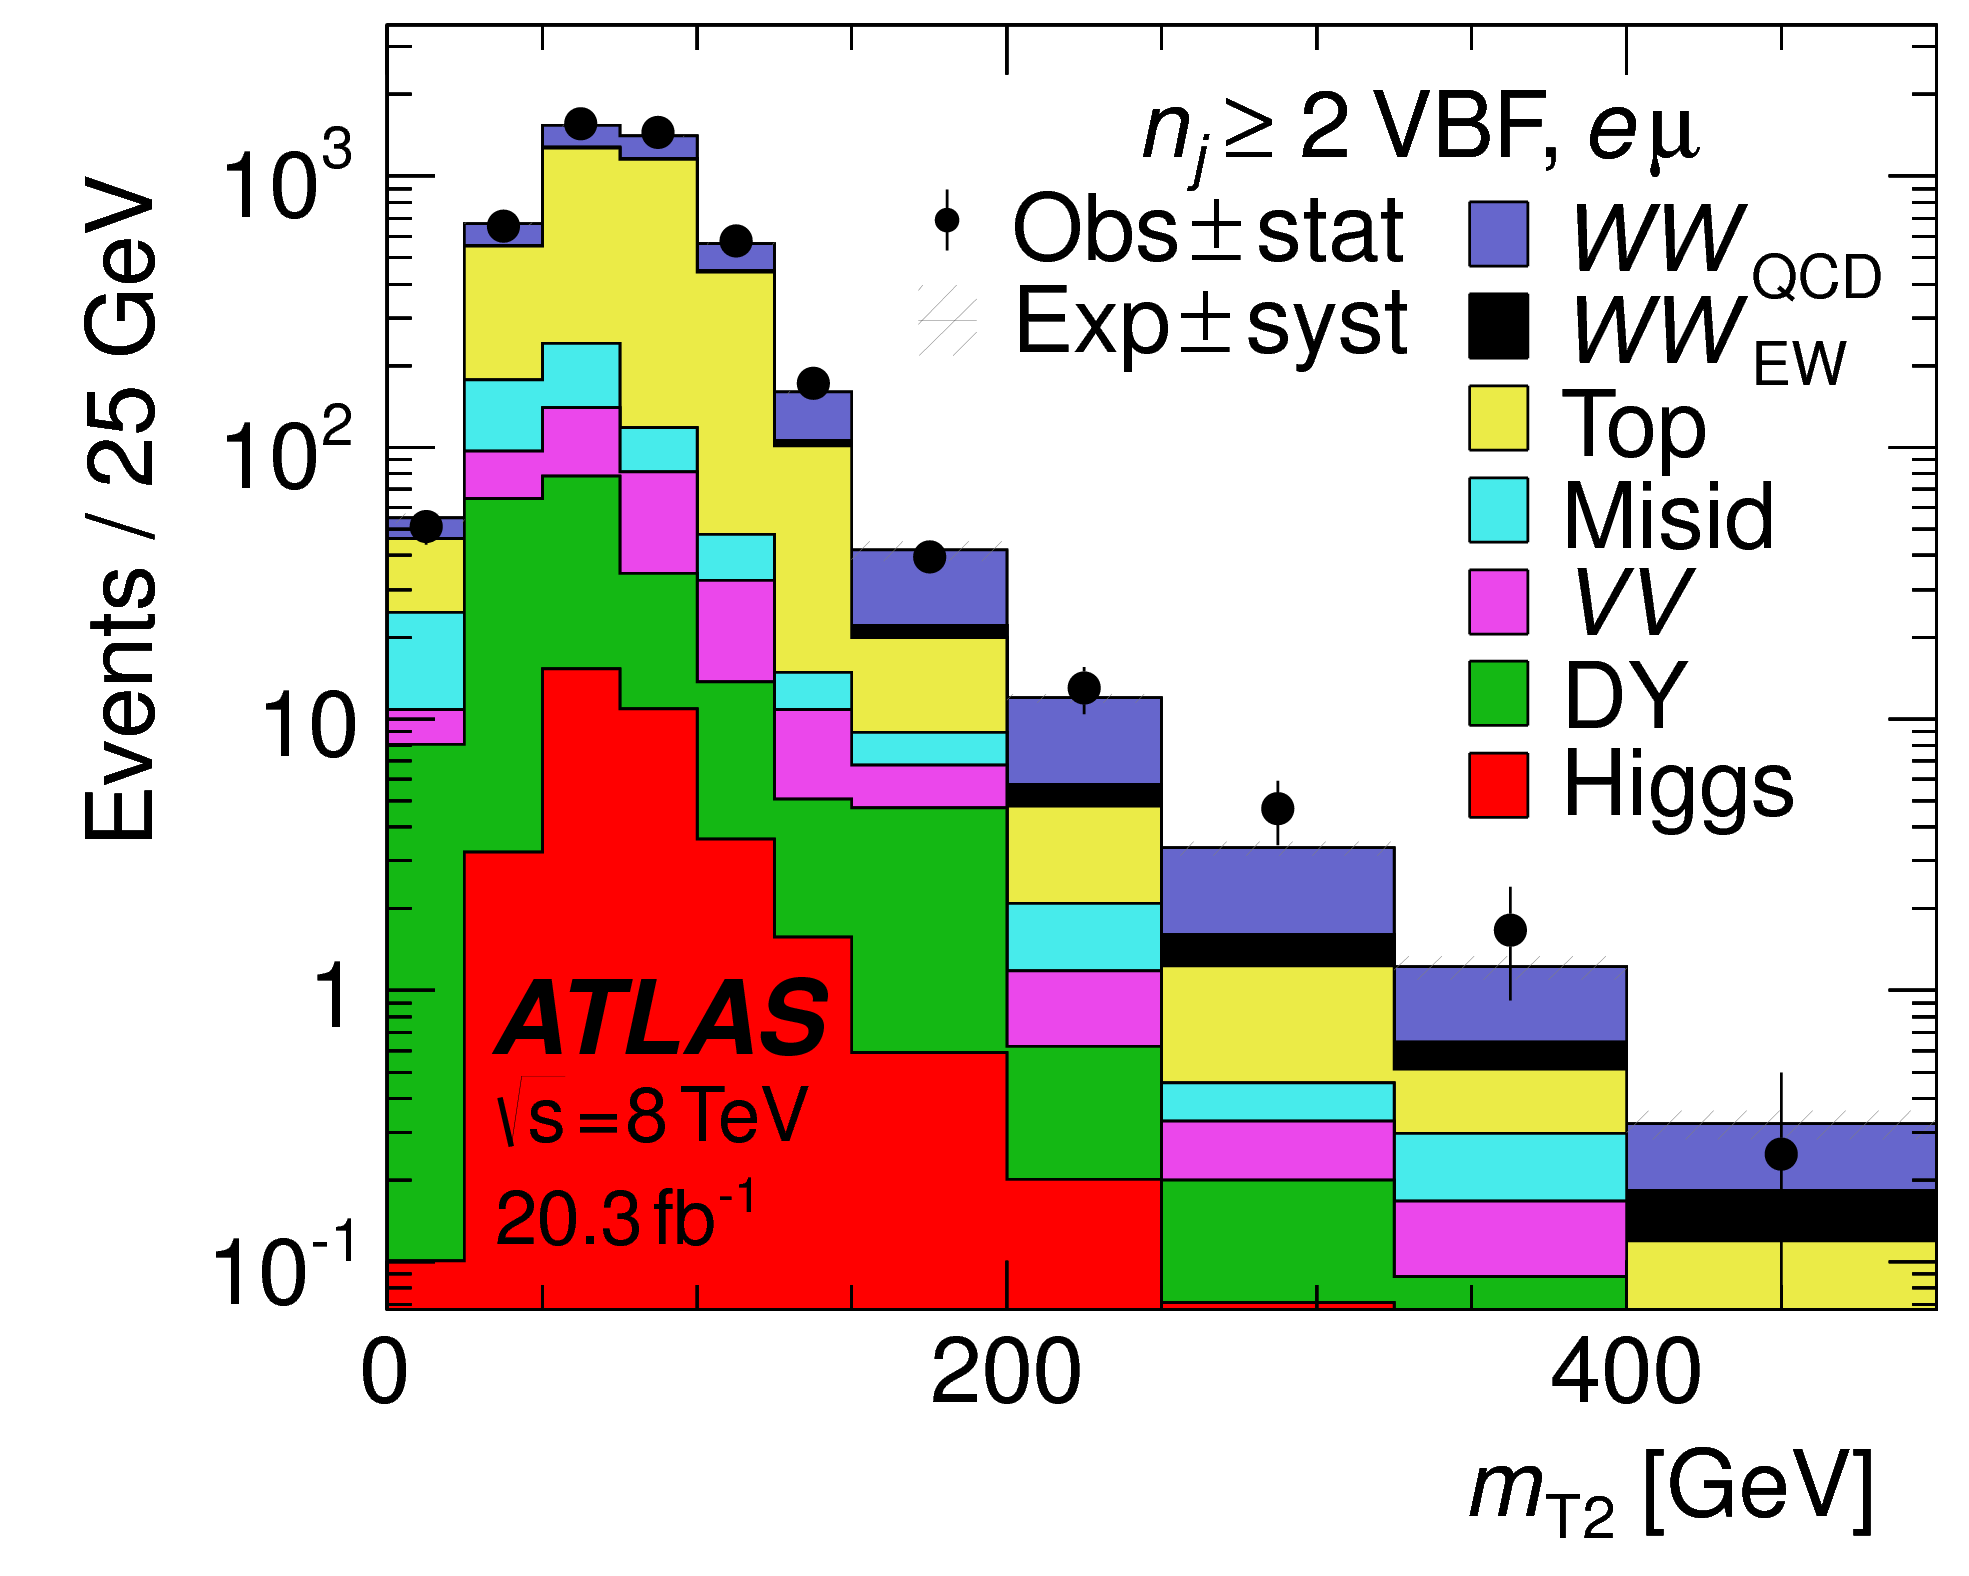
\includegraphics[width=0.5\textwidth]{figures/VBF_mT2}
  \caption{Distribution of $\mTtwo$ in the $WW$ validation region of the VBF analysis~\cite{WW2015}.}
  \label{fig:mt2}
\end{figure}

\subsection{Higgs production via gluon-gluon fusion}

Because this analysis is dedicated to measuring the VBF contribution to Higgs production, the component of Higgs production from gluon-gluon fusion is treated as a background. The shape is taken directly from simulation, using the generators described in table~\ref{tab:HWW-MC}. In the final combined fit of all different Higgs signal regions, the normalization is controlled by either a combined signal strength parameter $\mu$, which controls the normalization of both ggF and VBF production, or a separate parameter $\mu_{\rm ggF}$ depending on the interpretation being presented in the final results.  

\subsection{Backgrounds with misidentified leptons}

As discussed previously, the $W+$jets and QCD multijet backgrounds are derived with fully data-driven methods. These backgrounds do not make a large contribution to the final VBF signal region but their estimation methods are discussed briefly here. Because both backgrounds involve at least one mis-identified lepton, they are labeled as ``misid" throughout this chapter.

\subsubsection{$W$+jets background}

The $W$+jets background enters the signal region by having one of the jets mis-reconstructed as a lepton. The background is estimated by constructing a control sample with two leptons, where one lepton passes the usual lepton quality requirements but the second lepton fails one of those requirements (also known as the ``anti-identified" lepton). This control region is rich in the $W$+jets contribution because if a second lepton is reconstructed in a $W$+jets event it is likely to be of poor quality. The purity of this $W$+jets control sample is $85$\% to $90$\% depending on the exact configuration of leptons in the final state.

The $W$+jets content of the signal region is estimated by extrapolation from the control sample to the signal region using extrapolation factors derived in a $Z$+jets control sample in data. The assumption of the method is that the probability of a jet being misidentified as a lepton does not change between $W$+jets and $Z$+jets samples, and systematic uncertainties are assigned for differences in sample composition. The extrapolation factor is defeined as the ratio of the number of lepton candidates satisfying all quality criteria to the number of lepton candidates anti-identified. This ratio is measured in bins of $\pT$ and $\eta$. Thus, the final signal region estimate (binned as the extrapolation factor is binned) is simply the number of events in the anti-identified lepton control sample multiplied by the extrapolation factor derived from the $Z$+jets control sample. Figure~\ref{fig:VBF_extrap_Wjets} shows the extrapolation factors derived for electrons and muons.  The extrapolation factor can be seen in the figure to be an order of magnitude larger for muons than electrons, but this does not indicate that jets have a larger probability to be mis-identified as a muon than an electron. Values of the extrapolation factor are actually determined by the specific requirements used to define an anti-identified lepton. The difference between the muon and electron extrapolation factors comes from different definitions of the anti-identified lepton in each case.

\begin{figure}[h!]
  \centering
  \captionsetup{justification=centering}
  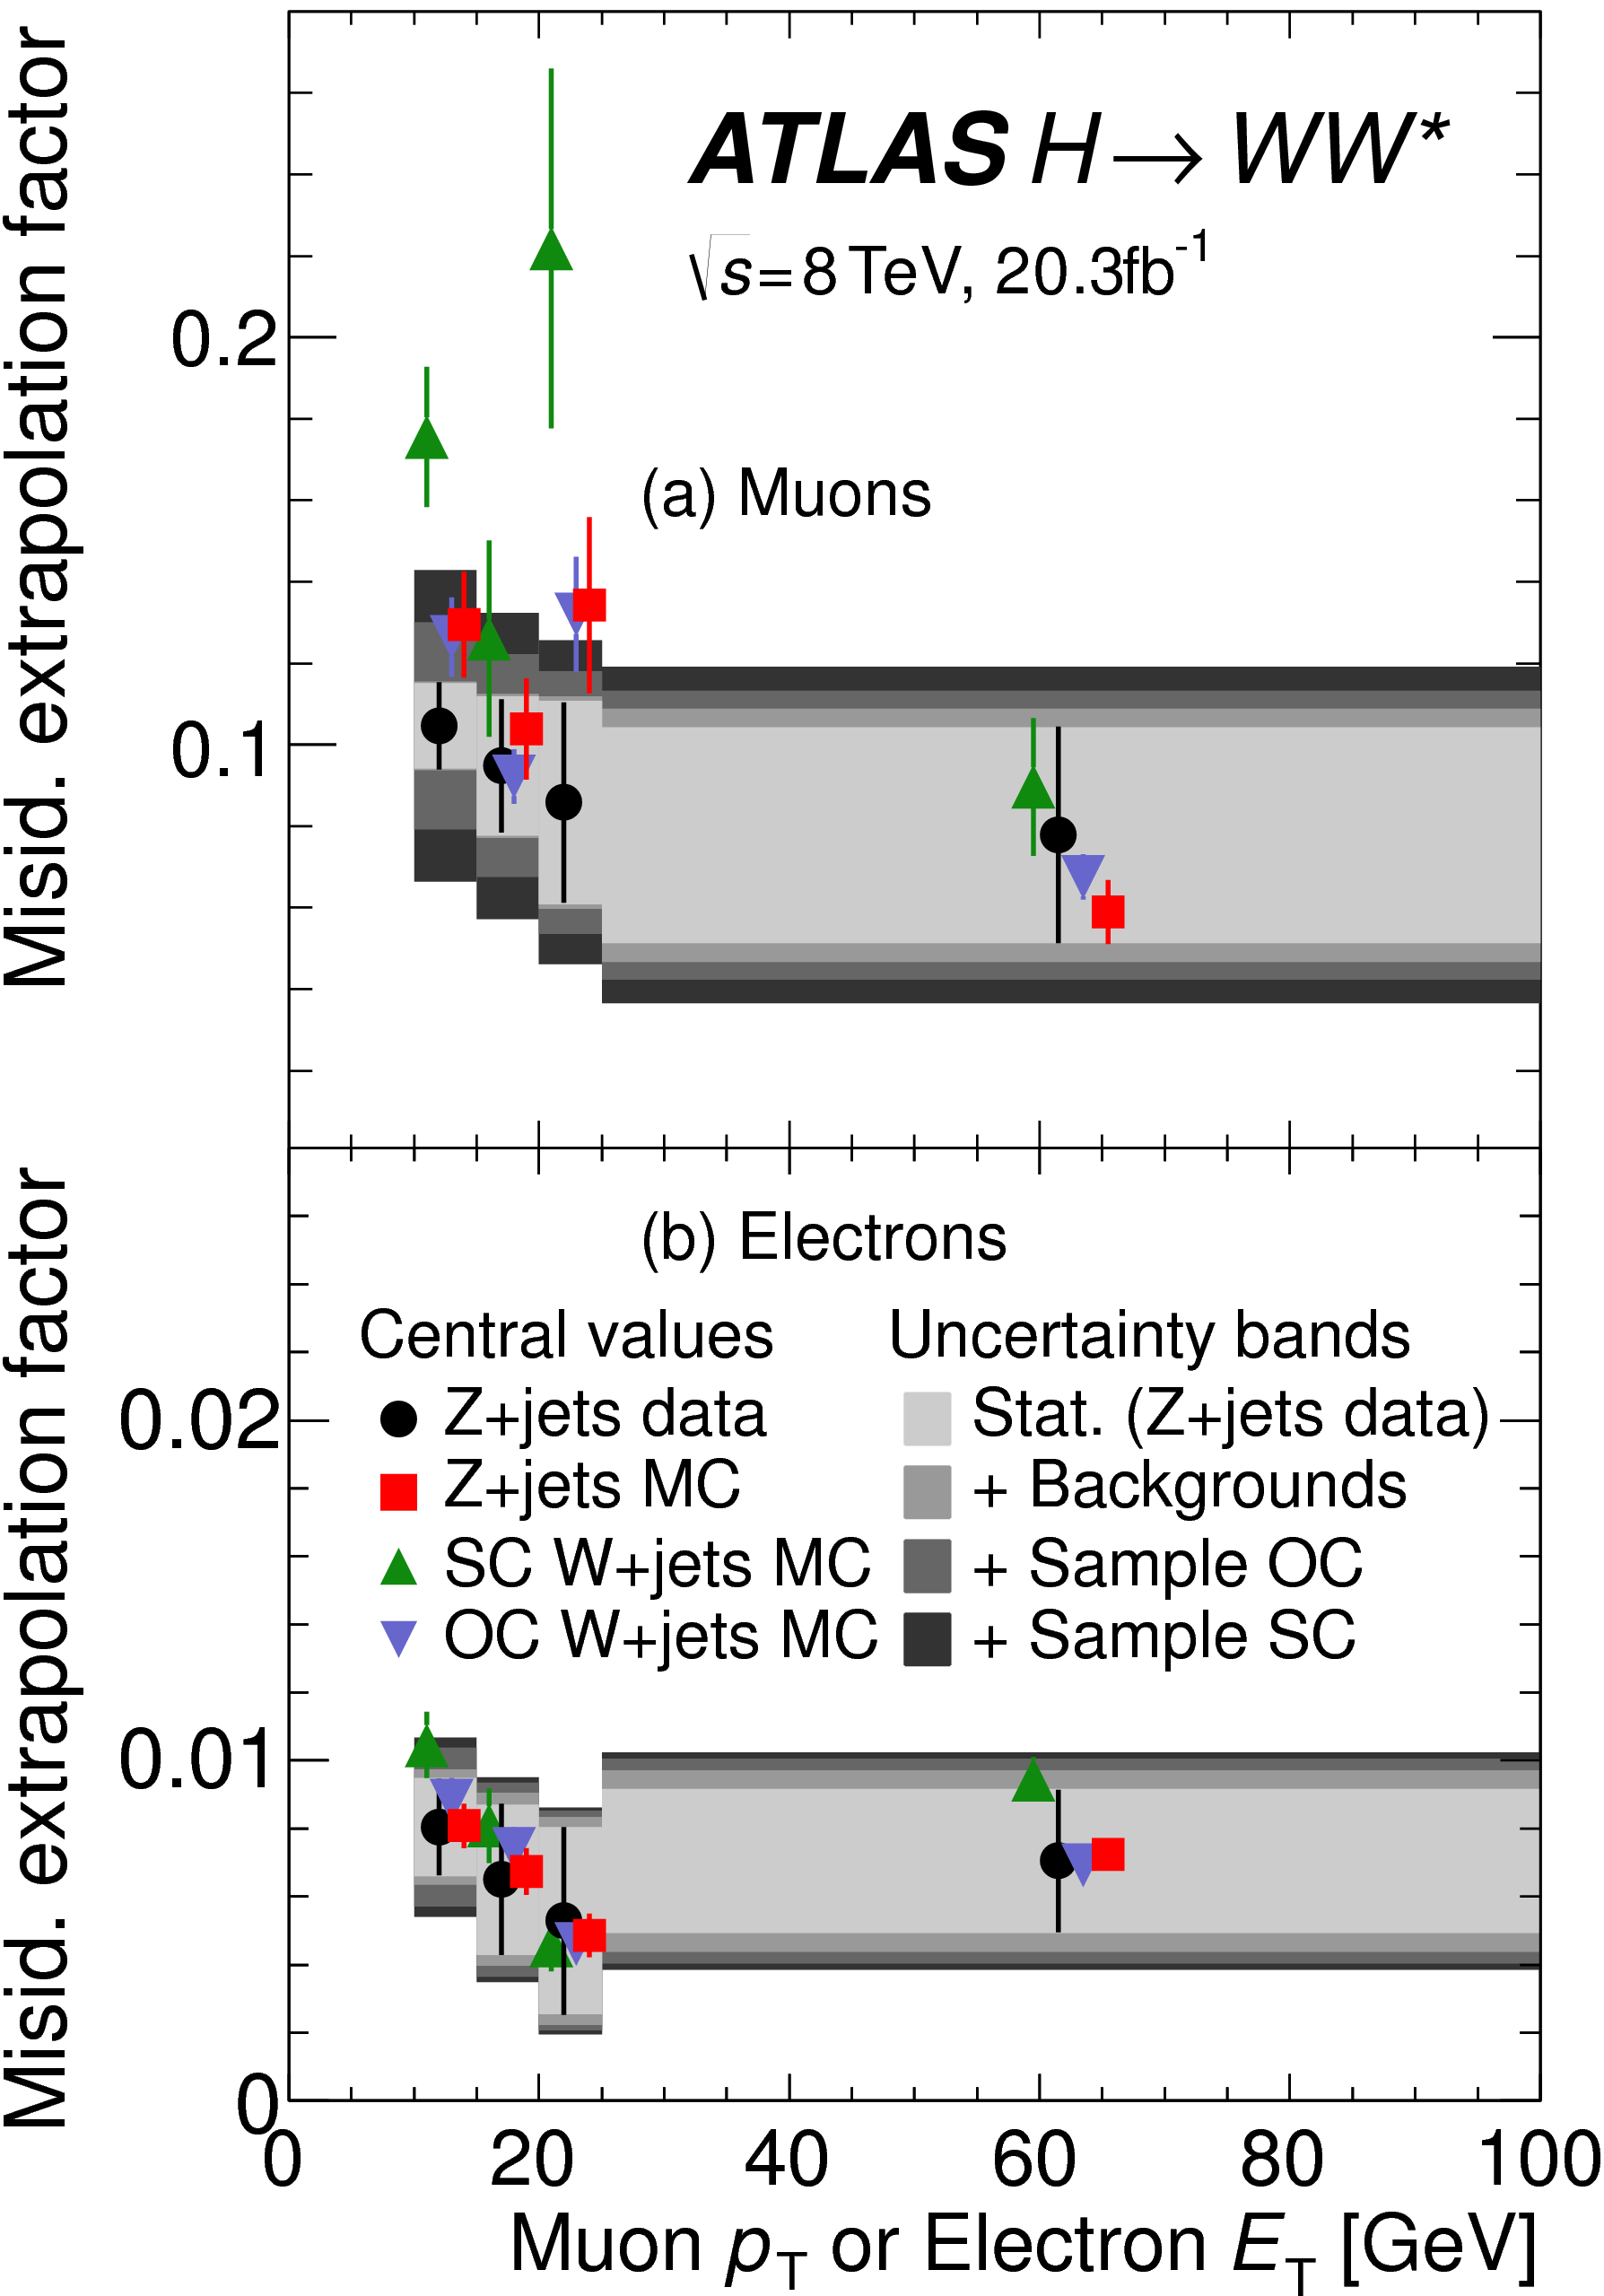
\includegraphics[width=0.55\textwidth]{figures/VBF_Wjets_extrap}
  \caption{Extrapolation factors for the $W$+jets estimate derived for muons (a) and electrons (b) as a function of lepton~$\pT$~\cite{WW2015}. OC refers to the opposite charge $W$+jets MC sample, while SC refers to the same charge $W$+jets MC. The uncertainty bands have contributions from statistical uncertainty in the data and backgrounds to $Z$+jets that are subtracted from the data, as well as systematic uncertainties due to variations in the extrapolation factor between the three MC samples shown.}
  \label{fig:VBF_extrap_Wjets}
\end{figure}

\subsubsection{QCD multijet background}

The method for estimating the multijet background is very similar to the $W$+jets estimation method. The control sample in this case has two anti-identified leptons but otherwise satisfies all signal region requirements. The extrapolation factor is estimated from a multijet sample and applied twice to the control sample. 

\subsection{Background composition in signal region}

After all of these estimation procedures, the signal region background composition can be calculated. The estimated yields are all shown in table~\ref{tab:vbf_cutflow_bkg}. Figure~\ref{fig:VBF_bkg_comp} shows the relative percentages of the different background for the different flavor and same flavor final states. In $e\mu$, the leading backgrounds are top backgrounds, ggF Higgs, and SM $WW$ production. In $ee/\mu\mu$, the leading background is Drell-Yan, followed by top and ggF Higgs.


\begin{figure}[h!]
  \centering
  \captionsetup{justification=centering}
  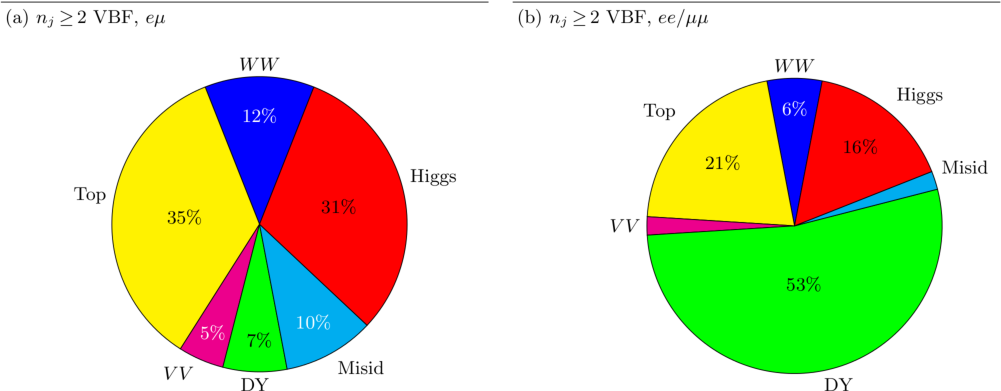
\includegraphics[width=\textwidth]{figures/VBF_bkg_comp}
  \caption{Background composition in final VBF signal region~\cite{WW2015}.}
  \label{fig:VBF_bkg_comp}
\end{figure}

\section{Systematic uncertainties}

There are two main types of systematic uncertainties that are assessed for the analysis. First, theoretical uncertainties associated with the signal and background yield estimates are discussed. Then, experimental uncertainties due to detector effects are shown. Normalization uncertainties refer to uncertainties that affect the cross section of the process in question in the signal region being probed. Shape uncertainties refer to systematic uncertainties that affect the shape of the final discriminating variable (either $\mTH$ or $\bdt$). 

\subsection{Theoretical uncertainties}
\label{sec:theory_uncert_WW}

There are four main components to theoretical uncertainties assigned to signal and background processes taken from Monte Carlo. Each one is a different source of variation in the overall acceptance for that process. The first involves variation of the QCD renormalization and factorization scales used in the calculation. In this case, the two scales are varied both independently and simultaneously by factors of two high or low. The resulting variation in normalization and shape for the process is taken as a systematic uncertainty (referred to as scale uncertainty). This uncertainty approximates the level of the correction to the cross section that would come from including the next order of the QCD calculation. Next, there is an uncertainty associated with the PDF set used in generating the events. The uncertainty eigenvectors for the given PDF set are inspected, and the envelope of maximal variation is taken as an uncertainty  (referred to as PDF uncertainty). Finally, there are two uncertainties associated with the choice of MC software. An uncertainty associated with the generator chosen for the hard scattering process is evaluated by keeping the parton showering software constant but varying the matrix element generator and taking the maximal variation as an uncertainty (referred to as the generator uncertainty). The converse variation can also be done, where the matrix element generator remains constant and the generator used for the underlying event/parton shower modeling is varied (referred to as the UE/PS uncertainty). In cases where the background is normalized in a control region, the systematic uncertainty arises from variations of the extrapolation factor $\alpha$ between the CR and the SR, which can affect the normalization of the background in the SR. 

%\begin{table}[h!]
%\centering
%\captionsetup{justification=centering}
%\begin{tabular}{|c|c|c|c|c|}
%\hline
%& VBF $H$ & ggF $H$ & Top & QCD $WW$  \\ \hline

%Total $\sigma$ & $2.7$ & $7.2$ & - & - \\ \hline
%Jet binning & - & $29$ & - & - \\ \hline
%Scale & $3.0$ & $48$ & $5.0$ & $27^*$ \\ \hline
%Generator & $4.2$ & - & $21$ & $12$ \\ \hline
%PDF & - & $3.0$ & - & $4^*$ \\ \hline
%UE/PS & $14$ & $15$ & - & $2$ \\ \hline
%\end{tabular}
%\caption{Systematic uncertainties for various processes in the BDT analysis, given in units of \% change in yield. Values are given for the most sensitive BDT bin (bin 3), except where noted with a *, in which case the uncertainty affect the normalization in all BDT bins. Empty entries indicate that the uncertainty is negligible or not applicable to this background.}
%\label{tab:vbf_bdt_theosys}
%\end{table}

There are two additional uncertainties that are applied to the Higgs processes as well. First, there are uncertainties assigned to the Higgs total production cross section. Then, there are uncertainties assigned based on the fact that the analysis is done in exclusive jet bins and it is possible for signal events to migrate from one bin to the next depending on the presence or absence of jets. These are assigned using the Jet Veto Efficiency (JVE) procedure~\cite{LHCXSWG,JVE} for ggF events and the Stewart-Tackmann (ST) method~\cite{ST} for VBF production. Table~\ref{tab:vbf_cb_theosys} shows the total theory uncertainties on the backgrounds in the cut-based analysis. These are the sum in quadrature of the uncertainties from each of the variations described above. 

%Table~\ref{tab:vbf_bdt_theosys} shows how the different theory uncertainty components contribute to variation in the yields of dominant background processes and signal in the BDT analysis. 

\begin{table}[h!]
\centering
\captionsetup{justification=centering}
\begin{tabular}{|c|c|}
\hline
Process & Theory syst. (\%)  \\ \hline
ggF $H$ & $48$ \\ \hline
Top & $26$ \\ \hline
QCD $WW$ & $37$ \\ \hline
$\ZDY \to \tau\tau$ & $6.1$ \\ \hline
\end{tabular}
\caption{Theoretical systematic uncertainties for various processes in the cut-based VBF analysis, given in units of \% change in yield. Values are given for the low $\mjj$ signal region.}
\label{tab:vbf_cb_theosys}
\end{table}

Figures~\ref{fig:vbf_tt_pdf} and~\ref{fig:vbf_tt_qcd} show the variations in the extrapolation factor from the PDF and QCD uncertainties on the top background estimate, binned in $\mTH$, for the cut-based analysis. In both cases, there was no significant shape uncertainty but normalization uncertainties were assigned according to the maximal variation. These uncertainties enter into the $26\%$ total uncertainty on top quark production quoted in table~\ref{tab:vbf_cb_theosys}

While the estimate for the same-flavor $\ZDY\to\ell\ell$ background is data-driven, there is still a systematic uncertainty taken for the non-closure of the method in Monte Carlo. This is taken as the maximum of the deviation of the non-closure factor $f_{\rm corr}$ from unity and its uncertainty, or $\textrm{max}(|1 - f_{\rm corr}|, \delta f_{\rm corr})$. For the cut-based analysis this non-closure uncertainty $23$\%, while for the BDT analysis it is $17\%$.

\begin{figure}[h!]
  \centering
  \captionsetup{justification=centering}
  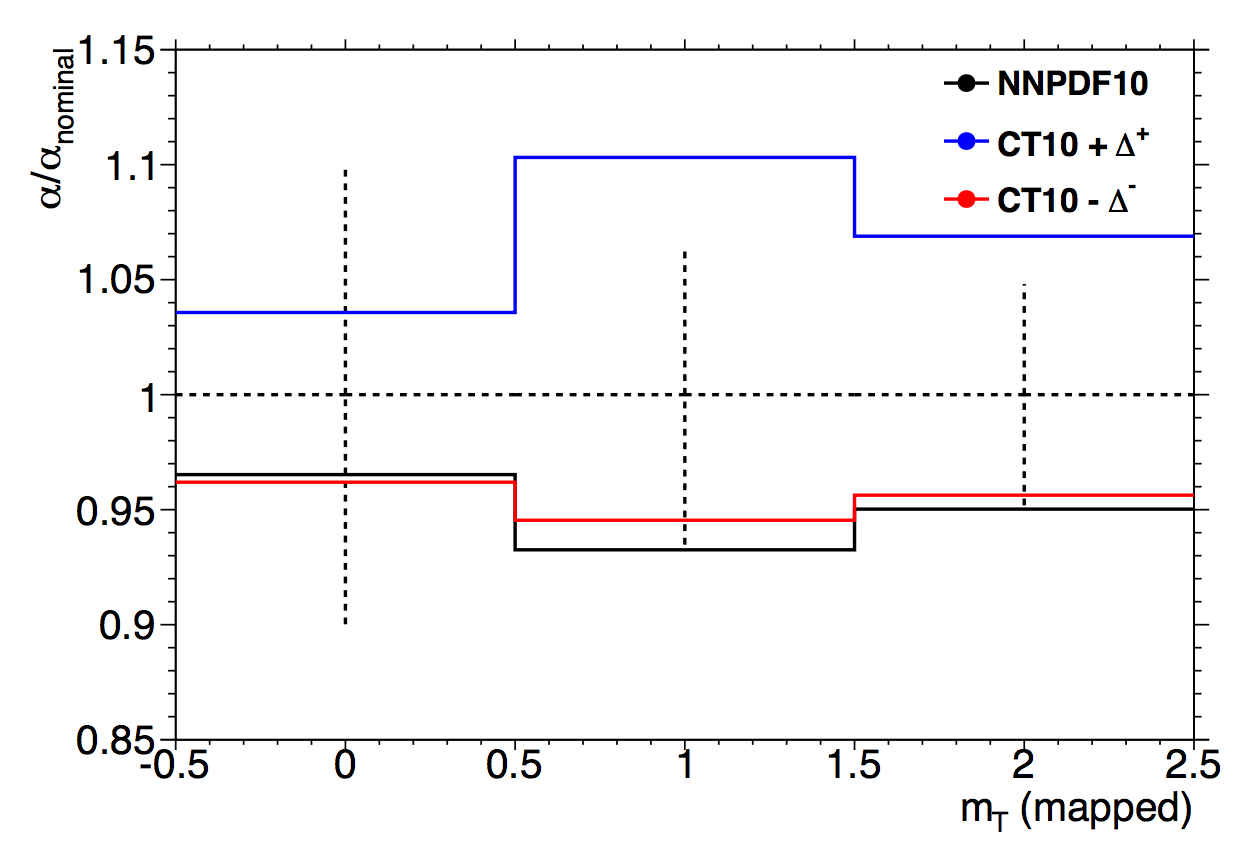
\includegraphics[width=0.7\textwidth]{figures/VBF_cb_tt_pdf}
  \caption{Variations in the top background extrapolation factor in the cut-based analysis due to PDF uncertainties. The uncertainties are shown in the three bins of $\mTH$ used in the final cut-based statistical fit. Variations from the eigenvector of the nominal PDF, \CT10, as well as the result from an alternate PDF (\NNPDF10), are compared.}
  \label{fig:vbf_tt_pdf}
\end{figure}

\begin{figure}[h!]
  \centering
  \captionsetup{justification=centering}
  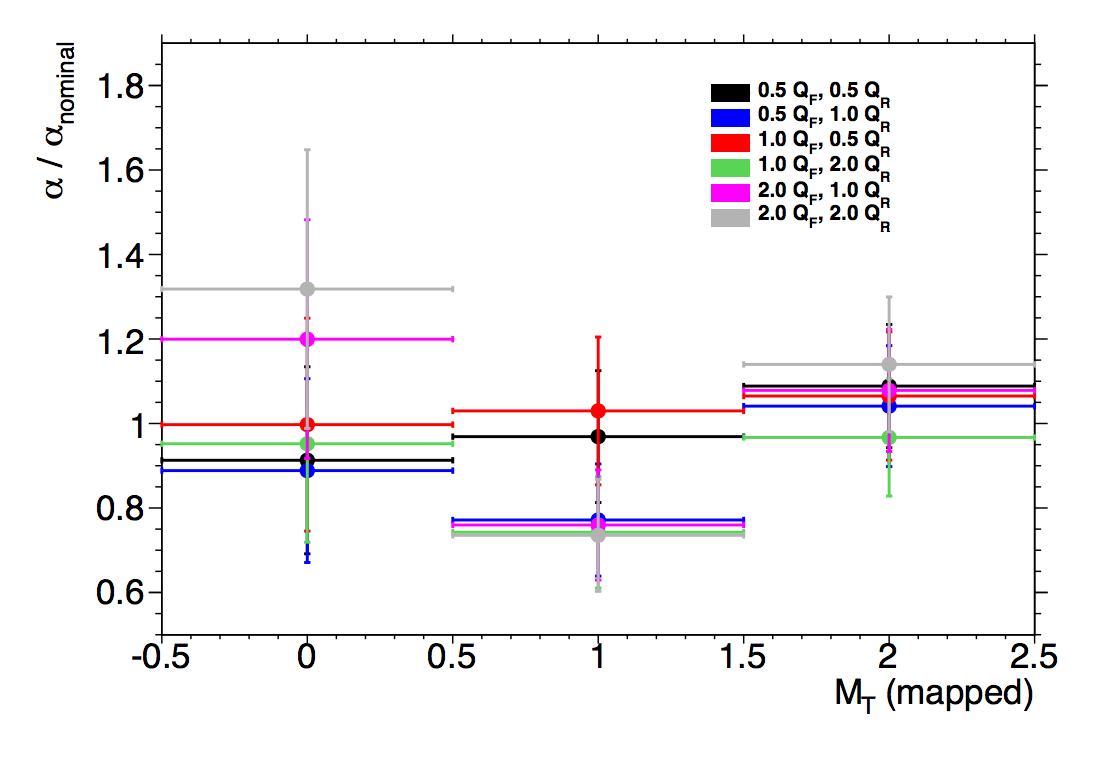
\includegraphics[width=0.7\textwidth]{figures/VBF_cb_tt_qcd}
  \caption{Variations in the top background extrapolation factor in the cut-based analysis due to QCD scale uncertainties. The uncertainties are shown in the three bins of $\mTH$ used in the final cut-based statistical fit. $Q_{F}$ is the QCD factorization scale, while $Q_{R}$ is the QCD renormalization scale.}
  \label{fig:vbf_tt_qcd}
\end{figure}

\subsection{Experimental uncertainties}

In this analysis, the theoretical uncertainties are the most dominant after statistical, but there are some experimental uncertainties that make a contribution as well. The first is the uncertainty on the measured integrated luminosity, which affects the signal estimate and backgrounds whose normalizations are taken from MC. It is measured to be $2.8$\% in the $8 \TeV$ dataset~\cite{luminosity-paper}. The dominant sources of uncertainty overall are uncertainties on the jet energy scale and resolution and the $b$-tagging efficiency. Additional sources include lepton uncertainties on identification, resolution, and trigger efficiency, as well as uncertainties on the missing transverse momentum. 

The jet energy scale uncertainty is split into several independent components, including jet-flavor dependent calorimeter response uncertainties, uncertainties on modeling of pile-up interactions, uncertainties on extrapolation from the central to forward detector regions, and MC non-closure~\cite{atlas_jets}. The uncertainty on energy scale for jets used in this analysis ranges from $1\%$ to $7\%$ depending on the jet $\pT$ and $\eta$. The jet energy resolution varies from $5\%$ to $20\%$, with uncertainties ranging from $2\%$ to $40\%$ (the largest uncertainties occurring at the selection threshold).

The b-tagging efficiency is independently measured in data samples enriched in dileptonic decays of $\ttbar$ events or in events where a muon is reconstructed in the vicinity of a jet~\cite{btag-calib,btag-muons}. The efficiencies and their uncertainties are binned in $\pT$ and decomposed into uncorrelated components using an eigenvector method~\cite{BtagCalib1}. Uncertainties on the efficiency range from $1\%$ to $7.8\%$. The uncertainty on the rate of misidentification of $c$-jets as $b$-jets ranges from $6$-$14$\%, while the uncertainty on the rate of light jet mis-tagging ranges from $9$-$19\%$ depending on $\pT$ and $\eta$. These efficiency uncertainties are applied to each individual jet in the event. 

Table~\ref{tab:vbf_exptsys} shows the effect of the experimental uncertainties on the VBF signal yield. The largest experimental uncertainty is the jet energy scale and resolution. Object uncertainties associated with $\MPTj$, electrons, and muons also make a small contribution, as well as the uncertainty on the trigger efficiency.

\begin{table}[h!]
\centering
\captionsetup{justification=centering}
\begin{tabular}{|c|c|}
\hline
Uncertainty source & \specialcell{Impact on \\signal yield (\%)}  \\ \hline
Jet energy scale and resolution & $5.4$ \\ \hline
Luminosity & $2.8$ \\ \hline
$\MPTj$ scale and resolution & $1.2$ \\ \hline
Electron uncertainties & $1.0$ \\ \hline
Muon uncertainties & $0.9$ \\ \hline
Trigger efficiency & $0.4$ \\ \hline
\end{tabular}
\caption{Experimental systematic uncertainties (expressed as \% of the estimated yield) for the VBF signal~\cite{WW2015}.}
\label{tab:vbf_exptsys}
\end{table}

The total experimental uncertainties on different signal and background components are summarized in table~\ref{tab:vbf_totsyst}. They are compared to the level of other statistical and systematic uncertainties as well. Overall, the experimental uncertainties are sub-dominant compared to the statistical and theoretical uncertainties.

\begin{table}[t!]
\centering
\captionsetup{justification=centering}

{\small
  \centering
\begin{tabular}{
    p{0.18\textwidth} 
    c
    c
    c
    c
}
\dbline
\multicolumn{1}{l}{Sample} & 
\multicolumn{1}{p{0.100\textwidth}}{~~~~Total} &
\multicolumn{1}{p{0.100\textwidth}}{~~~~Stat.$\nq$} & 
\multicolumn{1}{p{0.100\textwidth}}{~~~~Expt.} & 
\multicolumn{1}{p{0.100\textwidth}}{~~~~Theo.} \\
&
\multicolumn{1}{l}{~~~~uncert.}  &
\multicolumn{1}{l}{~~~~uncert.}  &
\multicolumn{1}{l}{~~~~uncert.}  &
\multicolumn{1}{l}{~~~~uncert.} \\
\multicolumn{3}{l}{$\NjetGEtwo$ VBF-enriched} \\
\quad $\Nsig$                   & $13  $& $-$ & $6.8 $& $12 $ \\
\quad $\Nbkg$                   & $9.2 $& $4.7$ & $6.4$ & $4.5 $\\
\qquad $\NWW$                   & $32  $& $-$ & $14$  & $28$  \\
\qquad $\Ntop$                  & $15  $& $9.6$ & $7.6 $& $8.5$ \\
\qquad $\Nfakes$                & $22  $& $-$ & $12  $& $19$  \\
\qquad $\NVV$                   & $20  $& $-$ & $12 $ & $15 $ \\
\qquad $\Ntautau$\,(DY)$\nqq$   & $40  $& $25 $& $31$  & $2.9$ \\
\qquad $\Nll$\,(DY)$\nqq$       & $19  $& $11 $  & $15$  & $-$\\
\dbline
\end{tabular}
}
\caption{
  Composition of the post-fit uncertainties (in $\%$) on the total signal ($\Nsig$),
  total background ($\Nbkg$), and individual background yields in the VBF analysis~\cite{WW2015}. ``Stat." refers to statistical uncertainties, ``Expt." refers to experimental systematic uncertainties, and ``Theo." refers to theoretical systematic uncertainties.
}
\label{tab:vbf_totsyst}
\end{table}
%eof

\section{Results}

While the combined results of all the $\HWW$ sub-analyses will be discussed in the next chapter, this section presents the results of the VBF specific analysis and interpretations. As table~\ref{tab:vbf_cutflow_summary} shows, the final cut-based signal region contains $20$ events in data with $\mTH < 150 \GeV$, $14$ coming from the $e\mu$ channel and $6$ coming from the $ee+\mu\mu$ channel. The BDT analysis has many more candidates due to its looser selection, and the yields in each bin of $\bdt$ are shown in table~\ref{tab:vbf_bdt_yield}. Most of the information about the VBF signal comes from bins $2$ and $3$ which have significantly better signal to background ratios than bin $1$. Additionally, the same-flavor channels contribute roughly the same sensitivity as the different flavor channels, highlighting the gain from adding these channels post-discovery with the techniques discussed in chapter 3. 

\begin{table}[!hbtp]
\centering
\captionsetup{justification=centering}
\scalebox{0.7}
{\small
  \centering%
%--------------------------------------------------------------------------------
%\begin{tabular*}{1\textwidth}{ l r@{$\PM$}l d{0}d{0}d{0}d{1}d{1} p{0.005\textwidth} d{0}d{0}d{0}d{0}d{0}d{0} d{1}d{1}d{0} d{2}d{1}d{1} }
%\begin{tabular*}{1\textwidth}{ l r@{$\PM$}l ccccc p{0.005\textwidth} cccccc ccc ccc }
\begin{tabular}{ l r@{$\PM$}l ccccc p{0.005\textwidth} cccccc ccc ccc }
\\
\multicolumn{15}{l}{$\no$(a) Before the BDT classification}\\
\dbline
&\multicolumn{7}{c}{Summary}
&&\multicolumn{10}{c}{Composition of $\Nbkg$}
\\
\clineskip\cline{2-8}\cline{10-19}\clineskip
\multicolumn{1}{p{0.165\textwidth}}{Selection}
& \multicolumn{2}{p{0.050\textwidth}}{$\Nobs/\Nbkg\nq$}
& \multicolumn{1}{p{0.040\textwidth}}{$\Nobs\nq\no$}
& \multicolumn{1}{p{0.040\textwidth}}{$\Nbkg\np$}
& \multicolumn{3}{p{0.125\textwidth}}{~~~~~~$N_{\rm signal}$}
&
& \multicolumn{2}{l}{~~~~~$\NWW$}
& \multicolumn{2}{l}{~~~~~$\Ntop$}
& \multicolumn{2}{l}{~\,$\Nfakes$}
& \multicolumn{1}{p{0.048\textwidth}}{$~~~\NVV$}
& \multicolumn{3}{l}{~~~~~~~$\Ndrellyan$}
\\
\multicolumn{2}{l}{}
& 
& 
& 
& \multicolumn{1}{l}{$\NggF\no$}
& \multicolumn{1}{l}{$\NVBF\no$}
& \multicolumn{1}{l}{$\NVH\no$}
&
& \multicolumn{1}{p{0.040\textwidth}}{$\NWWqcd$}
& \multicolumn{1}{p{0.035\textwidth}}{$\NWWew$}
& \multicolumn{1}{p{0.050\textwidth}}{~~~$\Nttbar\no$}
& \multicolumn{1}{p{0.035\textwidth}}{~$\Nt\nq$}
& \multicolumn{1}{p{0.035\textwidth}}{$\NWj\nq$}
& \multicolumn{1}{p{0.035\textwidth}}{$\Njj\nq$}
& 
& \multicolumn{1}{p{0.045\textwidth}}{$\Nll\nq$}
& \multicolumn{1}{p{0.040\textwidth}}{$~\,\Ntautauqcd\nq$}
& \multicolumn{1}{p{0.050\textwidth}}{$~\,\Ntautauew\nq$}
\\
\sgline
%$\DFchan$ sample        &1.00 &0.00 &61434 &61180 &85   &32   &26  &&1350 &68   &51810 &2970 &847   &308  &380   & 51    &3260  &46   \\
$\DFchan$ sample         &$1.04 $&$0.04 $&$718   $&$689   $&$13   $&$15   $&$2.0 $&&$90   $&$11   $&$327   $&$42   $&$29    $&$23   $&$31    $&$2.2    $&$130   $&$ 2  $ \\
$\SFchan$ sample         &$1.18 $&$0.08 $&$469   $&$397   $&$ 6.0 $&$ 7.7 $&$0.9 $&& $37  $& $3   $&$132   $&$17   $&$ 5.2  $&$1.2  $&$10.1  $&$168    $&$ 23   $&$ 1  $ \\
\dbline
\\
\multicolumn{19}{l}{$\no$(b) Bins in $\bdt$}\\
\dbline
$\DFchan$ sample   \\
$\quad$ Bin 0 (not used) &$1.02 $&$0.04 $&$661   $&$650   $&$ 8.8 $& $3.0 $&$1.9 $&& $83  $& $9   $&$313   $&$40   $&$26    $&$21   $&$28    $& $ 2.2  $&$126  $ &$ 1   $\\
$\quad$ Bin 1            &$0.99 $&$0.16 $&$ 37   $&$ 37   $&$ 3.0 $& $4.2 $&$0.1 $&& $5.0 $& $1.0 $&$ 17   $&$ 3.1 $&$ 3.3  $&$ 1.8 $&$ 2.6  $&   $-$  &  $4.0 $&$ 0.2 $\\
$\quad$ Bin 2            &$2.26 $&$0.63 $&$ 14   $&$  6.2 $&$ 1.2 $& $4.2 $&$-$   && $1.5 $& $0.5 $&$  1.8 $&$ 0.3 $&$ 0.4  $&$ 0.3 $&$ 0.8  $&   $-$  &  $0.3 $&$ 0.3 $\\
$\quad$ Bin 3            &$5.41 $&$2.32 $&$  6   $&$  1.1 $&$ 0.4 $& $3.1 $&$-$   && $0.3 $& $0.2 $&$  0.3 $&$ 0.1 $& $-$    & $-$   &$ 0.1  $&   $-$  &  $0.1 $& $0.1 $\\
\sgline
$\SFchan$ sample   \\
$\quad$ Bin 0 (not used) &$1.91 $&$0.08 $&$396   $&$345   $& $3.8 $& $1.3 $&$0.8 $&& $33  $& $2   $&$123   $&$16   $& $4.1  $&$1.1  $& $8.8  $&$137   $ & $20.5 $& $0.5 $\\
$\quad$ Bin 1            &$0.82 $&$0.14 $&$ 53   $&$ 45   $& $1.5 $& $2.2 $&$0.1 $&& $3.0 $& $0.5 $&$ 10.4 $&$ 1.8 $& $0.8  $&$0.2  $& $0.9  $&$ 26   $ &  $1.7 $& $0.1 $\\
$\quad$ Bin 2            &$1.77 $&$0.49 $&$ 14   $&$  7.9 $& $0.6 $& $2.5 $&$-$   && $0.8 $& $0.3 $&$  1.1 $&$ 0.2 $& $0.2  $&$-$    & $0.3  $&$  4.4 $ &  $0.3 $& $0.1 $\\
$\quad$ Bin 3            &$6.52 $&$2.87 $&$  6   $&$  0.9 $& $0.2 $& $1.7 $&$-$   && $0.1 $& $0.2 $&$  0.2 $&   $-$ & $-$    &$-$    &   $-$  &$  0.7 $ &  $-$ & $-$ \\
\dbline            
\end{tabular}%                                                                                    
%--------------------------------------------------------------------------                        
}
\caption{
  Event selection for the VBF BDT analysis.
  The event yields in (a) are shown after the pre-selection and the additional
  requirements applied before the BDT classification (see text).
  The event yields in (b) are given in bins in $\bdt$ after the classification~\cite{WW2015}.
}
\label{tab:vbf_bdt_yield}                                                                                                 
\end{table}

Figure~\ref{fig:vbf_cb_mt}(a) shows the final distribution of data candidates compared to the expected $\mTH$ distribution for signal and background in the cut-based signal region. The data are very consistent with a VBF Higgs hypothesis. Figure~\ref{fig:vbf_cb_mt}(b) shows where the data candidates fall in the two-dimensional binning of $\mTH$ and $\mjj$ used in the fit for the cut-based analysis. 
%
\begin{figure}[h!]
  \centering
  \captionsetup{justification=centering}
  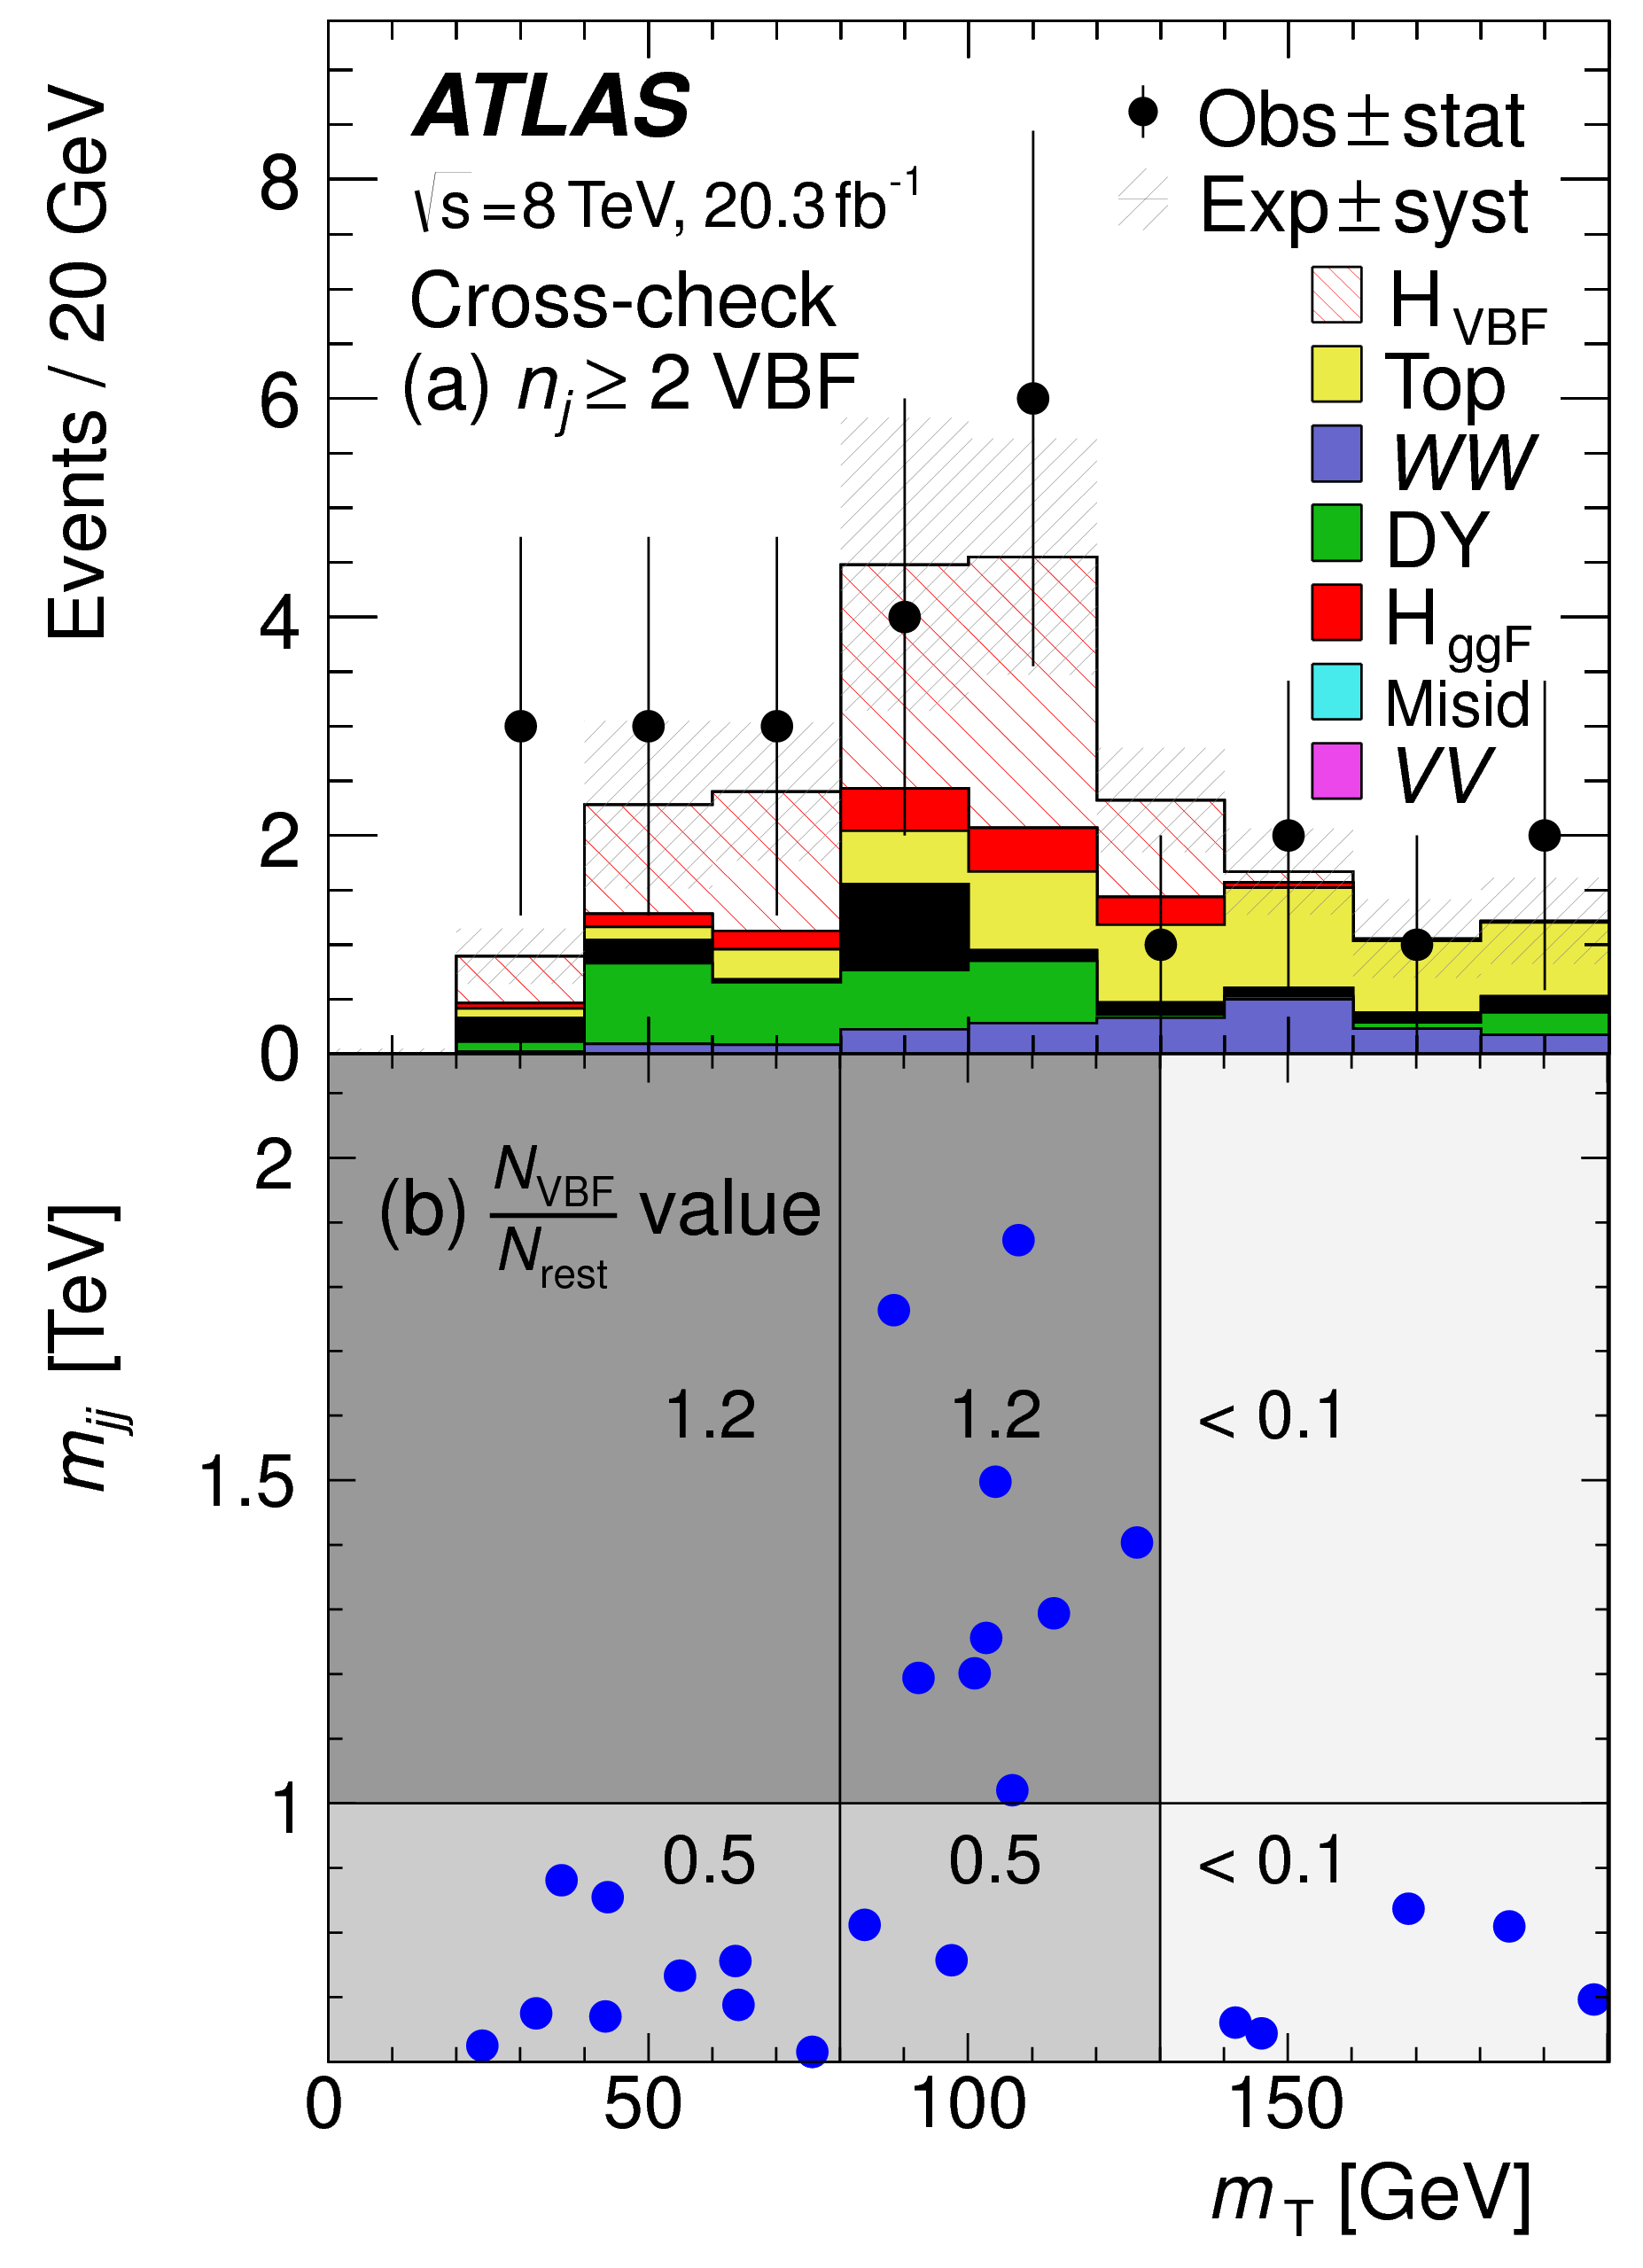
\includegraphics[width=0.7\textwidth]{figures/VBF_cb_mt}
  \caption{Post-fit distributions in the cut-based VBF analysis. Panel (a) shows the one-dimensional $\mTH$ distribution, while (b) shows the data candidates split into the bins of $\mTH$ and $\mjj$ used in the final fit~\cite{WW2015}.}
  \label{fig:vbf_cb_mt}
\end{figure}
%
Figure~\ref{fig:vbf_bdt_mt} shows the distributions of $\bdt$ and $\mTH$ in the VBF BDT analysis. Again the data are quite consistent with a VBF Higgs hypothesis. 
%
\begin{figure}[h!]
  \centering
  \captionsetup{justification=centering}
  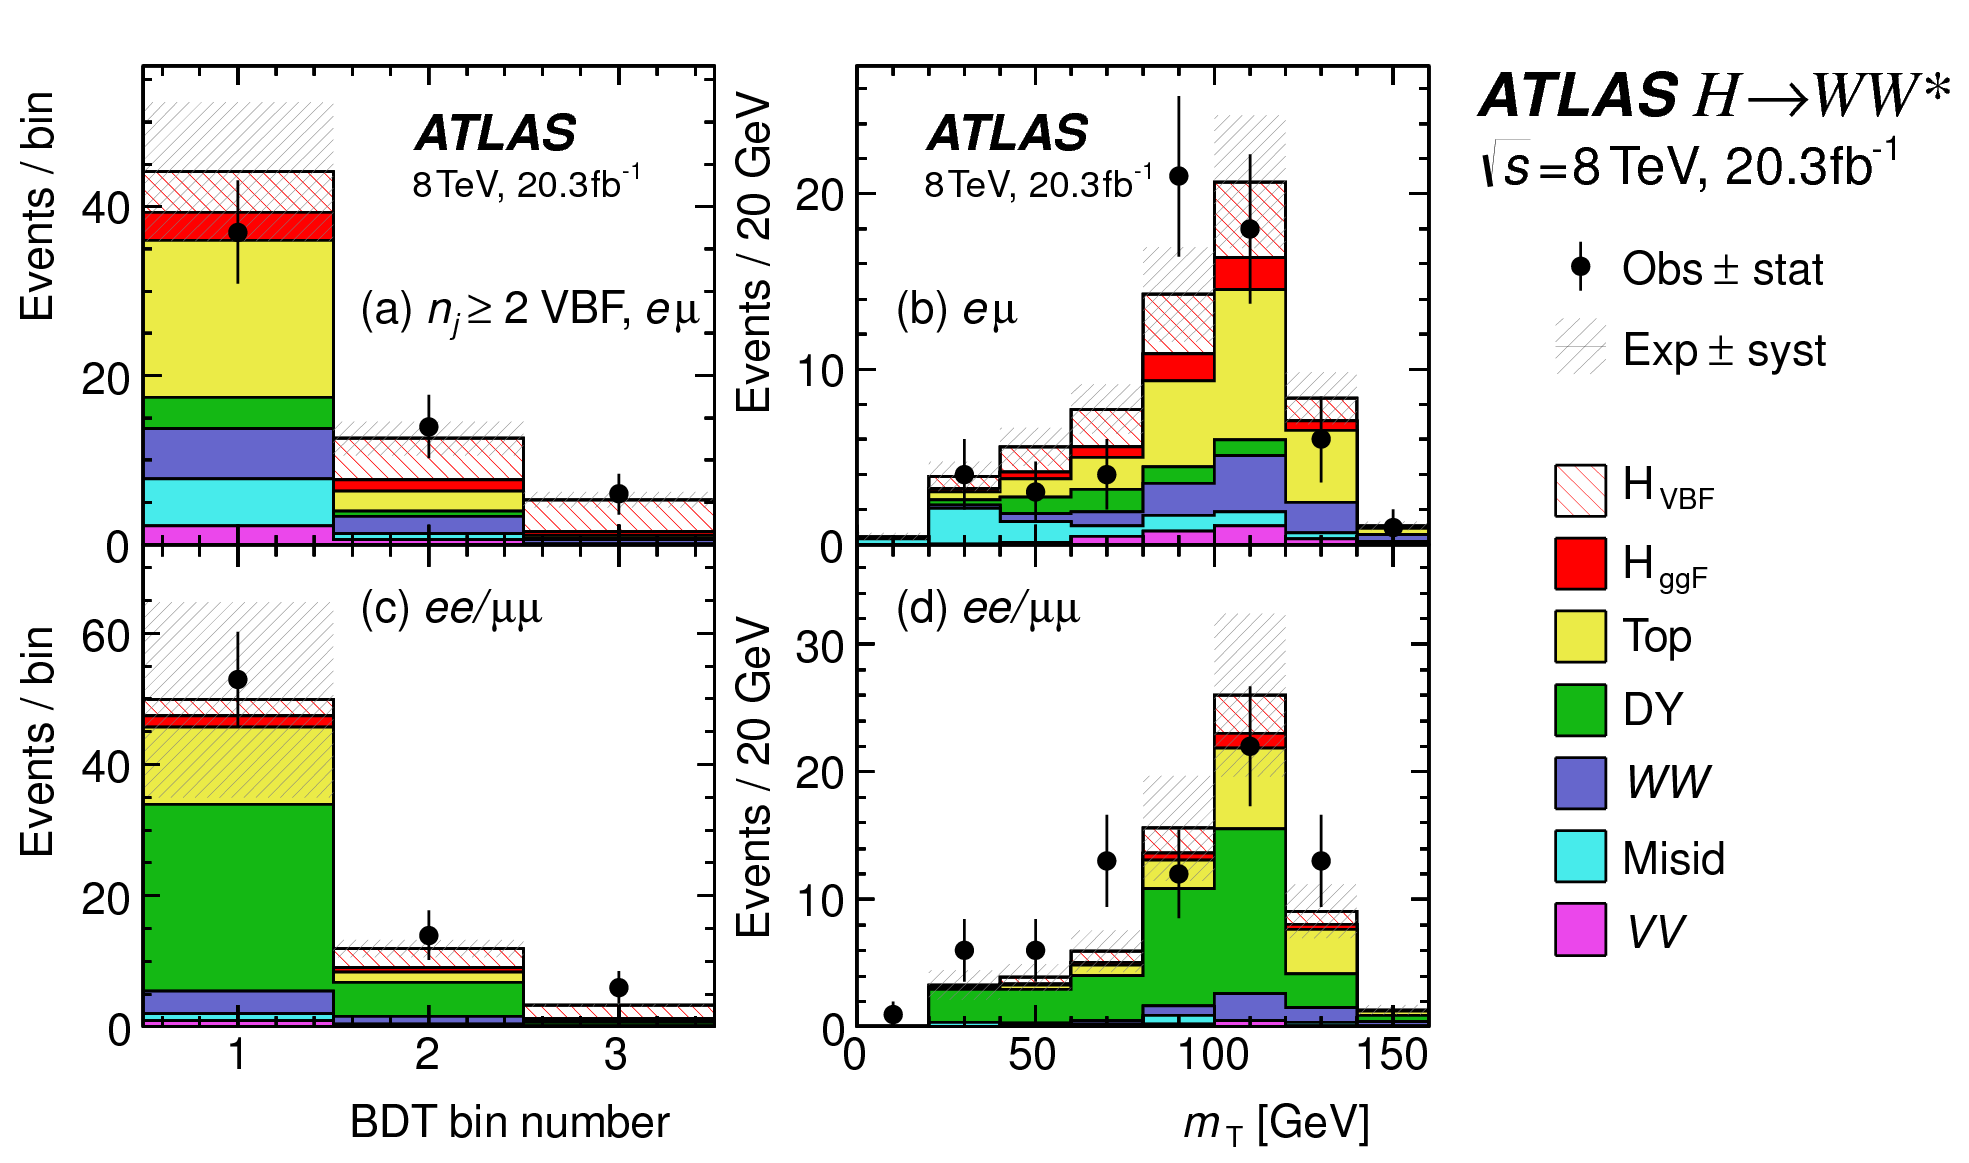
\includegraphics[width=0.8\textwidth]{figures/VBF_bdt_mt}
  \caption{Postfit distributions in the BDT VBF analysis~\cite{WW2015}.}
  \label{fig:vbf_bdt_mt}
\end{figure}

Because the cut-based result is used as a validation for the BDT analysis and the two signal regions are not fully orthogonal, it is interesting to explore which events overlap between the two analyses. Of the twenty events in the cut-based signal region, only seven were not selected by the BDT analysis, while the other thirteen also enter the BDT signal region. Figure~\ref{fig:vbf_bdt_cb_overlay} shows where the different analysis candidates lie in the $\mjj$-$\mTH$ plane. This shows clearly that the advantage of the BDT analysis is that it can extract signal candidates from the lower $\mjj$ region due to its ability to recognize correlations with other variables. 

\begin{figure}[h!]
  \centering
  \captionsetup{justification=centering}
  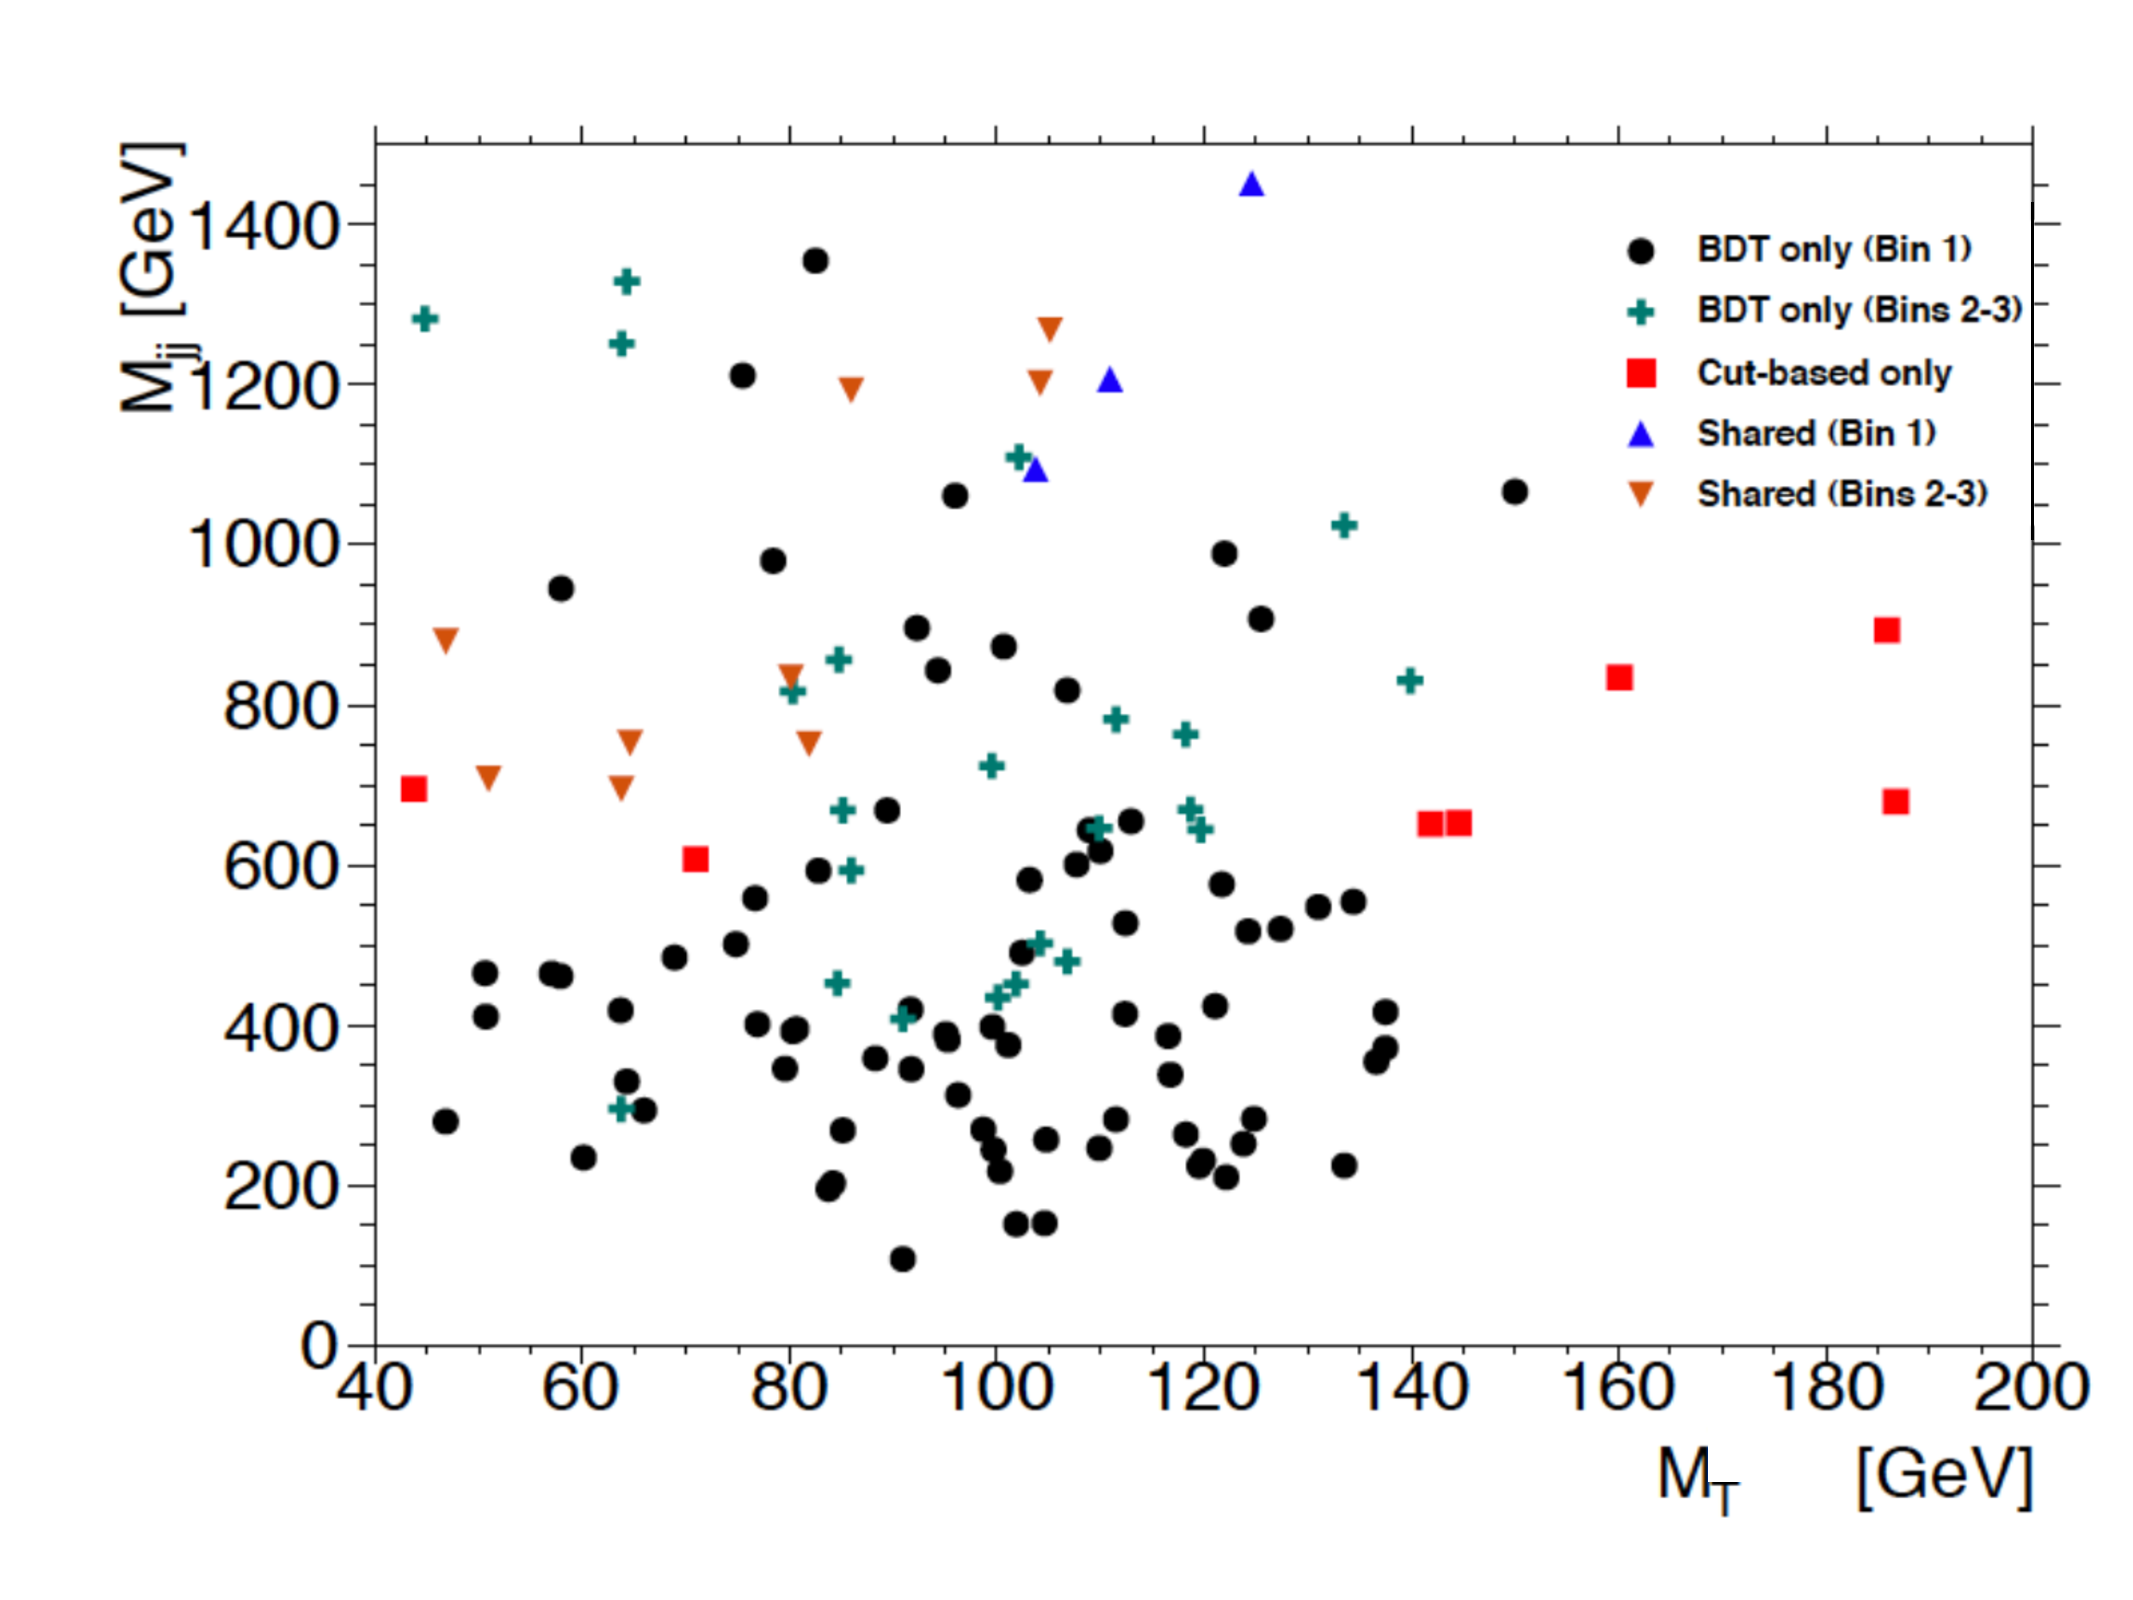
\includegraphics[width=0.8\textwidth]{figures/OverlapFig}
  \caption{Overlap between cut-based and BDT VBF signal region candidates in the $\mjj$-$\mTH$ plane.}
  \label{fig:vbf_bdt_cb_overlay}
\end{figure}

While the context of these results in the broader $\HWW$ statistical analysis will be presented in the next chapter, the statistical significance of the VBF Higgs result is shown here. In the BDT analysis, the expected signal significance was $2.7\sigma$, while the observed significance was $3.1\sigma$. In the cut-based analysis, the expected significance was $2.1\sigma$ and the observed significance was $3.0\sigma$. The compatibility between these two results can be evaluated by computing the probability of observing a larger difference in $Z_0$ values than the one measured. Using toy Monte Carlo with the ggF signal strength fixed to unity and considering only statistical uncertainties, this probability is computed to be $79\%$, indicating good agreement between the analyses. This result represents the first evidence of the vector boson fusion production of a Higgs boson. 
